\documentclass[12pt,a4paper]{report}

\usepackage{styles/dolgozat}

\usepackage{listings}
\usepackage{styles/cpp}
\usepackage{styles/python}
\usepackage{mathtools}
\usepackage{amsmath}

%\usepackage{styles/sql}
\DeclarePairedDelimiter{\floor}{\lfloor}{\rfloor}
\DeclarePairedDelimiter{\Bigfloor}{\left\lfloor}{\right\rfloor}
\usepackage{hyperref}

\begin{document}

\pagestyle{empty} %a címlapon ne legyen semmi=empty, azaz nincs fejléc és lábléc

% A Miskolci Egyetem címere
{\large
\begin{center}
\vglue 1truecm
\textbf{\huge\textsc{Szakdolgozat}}\\
\vglue 1truecm

\includegraphics[width=4.8truecm, height=4truecm]{images/me_logo.png}\\
\textbf{\textsc{Miskolci Egyetem}}
\end{center}}

\vglue 1.5truecm %függõleges helykihagyás

% A szakdolgozat címe, akár több sorban is
{\LARGE
\begin{center}
\textbf{A MySQL adatbázismotor teljesítményének optimalizálása OpenCL segítségével}
\end{center}}

\vspace*{2.5truecm}
% A hallgató neve, évfolyam, szak(ok), a konzulens(ek) neve
{\large
\begin{center}
\begin{tabular}{c}
\textbf{Készítette:}\\
Várady Dániel\\
Programtervező informatikus
\end{tabular}
\end{center}
\begin{center}
\begin{tabular}{c}
\textbf{Témavezető:}\\
Piller Imre
\end{tabular}
\end{center}}
\vfill
% Keltezés: Hely, év
{\large
\begin{center}
\textbf{\textsc{Miskolc, 2021}}
\end{center}}

\newpage


\newpage

\pagestyle{empty}

%Feladatkiiras
\begin{flushleft}
\textsc{\bfseries Miskolci Egyetem}\\
Gépészmérnöki és Informatikai Kar\\
Alkalmazott Matematikai Intézeti Tanszék\hspace*{4cm}\hfil \textbf{Szám:}
\end{flushleft}
\vskip 0.5cm
\begin{center}
\large\textsc{\bfseries Szakdolgozat Feladat}
\end{center}
\vskip 0.5cm
Várady Dániel (CGW85R) programtervező informatikus jelölt részére.\newline

\noindent\textbf{A szakdolgozat tárgyköre:} relációs adatbázis, MySQL, OpenCL\newline

\noindent\textbf{A szakdolgozat címe:} A MySQL adatbázismotor teljesítményének optimalizálása OpenCL segítségével\newline

\noindent\textbf{A feladat részletezése:}

\medskip

\emph{
A MySQL adatbázismotor egy széles körben használt, relációs adatmodellre épülő alkalmazás. A dolgozat célja, hogy megvizsgálja azokat az eseteket, amelyekben a számítási teljesítményt az OpenCL nyelv segítségével a több számítási maggal rendelkező konfigurációk esetén javítani lehet. A dolgozatban ehhez részletesen be kell mutatni a MySQL adatbázismotor felépítését, működésének a folyamatát, az SQL lekérdezések feldolgozási lépéseit. Példákat kell adni olyan lekérdezésekre, amelyek párhuzamosan végrehajthatók. Meg kell vizsgálni azt, hogy a feldolgozandó adatokat milyen struktúrákba célszerű rendezni, és azokat hogyan érdemes mozgatni a hatékonyabb számítások érdekében. Az eredmények szemléltetéséhez méréseket kell végezni adott hardveres konfiguráció mellett, amellyel objektív módon láthatóvá válnak az optimalizáció előnyei.
}

\vfill

\noindent\textbf{Témavezető:} Piller Imre (egyetemi tanársegéd) \newline

% \noindent\textbf{Konzulens(ek):} (akkor kötelezõ, ha a témavezetõ nem valamelyik matematikai tanszékrõl való; de persze lehet egyébként is)\newline

\noindent\textbf{A feladat kiadásának ideje:} 2019. szeptember 27.\newline

%\noindent\textbf{A feladat beadásának határideje:}

\vskip 2cm

\hbox to \hsize{\hfil{\hbox to 6cm {\dotfill}\hbox to 1cm{}}}

\hbox to \hsize{\hfil\hbox to 3cm {szakfelelős}\hbox to 2cm{}}

\newpage

\vspace*{1cm}  
\begin{center}
\large\textsc{\bfseries Eredetiségi Nyilatkozat}
\end{center}
\vspace*{2cm}  

Alulírott \textbf{Várady Dániel}; Neptun-kód: \texttt{CGW85R} a Miskolci Egyetem Gépészmérnöki és Informatikai Karának végzős Programtervező informatikus szakos hallgatója ezennel büntetőjogi és fegyelmi felelősségem tudatában nyilatkozom és aláírásommal igazolom, hogy \textit{A MySQL adatbázismotor teljesítményének optimalizálása OpenCL segítségével}
című szakdolgozatom saját, önálló munkám; az abban hivatkozott szakirodalom
felhasználása a forráskezelés szabályai szerint történt.\\

Tudomásul veszem, hogy szakdolgozat esetén plágiumnak számít:
\begin{itemize}
\item szószerinti idézet közlése idézőjel és hivatkozás megjelölése nélkül;
\item tartalmi idézet hivatkozás megjelölése nélkül;
\item más publikált gondolatainak saját gondolatként való feltüntetése.
\end{itemize}

Alulírott kijelentem, hogy a plágium fogalmát megismertem, és tudomásul veszem, hogy
plágium esetén szakdolgozatom visszautasításra kerül.

\vspace*{3cm}

\noindent Miskolc, \hbox to 2cm{\dotfill} .év \hbox to 2cm{\dotfill} .hó \hbox to 2cm{\dotfill} .nap

\vspace*{3cm}

\hspace*{8cm}\begin{tabular}{c}
\hbox to 6cm{\dotfill}\\
Hallgató
\end{tabular}



\newpage

\noindent 1.

\begin{tabular}{cl}
&szükséges (módosítás külön lapon) \\
A szakdolgozat feladat módosítása& \\
& nem szükséges\\
&\\
\hbox to 4cm{\dotfill}&\multicolumn{1}{c}{\hbox to 5cm{\dotfill}}\\
dátum& \multicolumn{1}{c}{témavezető(k)}
\end{tabular}
\vskip1.5mm

\noindent 2. A feladat kidolgozását ellenőriztem:

\vskip1.5mm

\begin{tabular}{l@{\hspace*{4cm}}l}
témavezető (dátum, aláírás):& konzulens (dátum, aláírás):\\
\dotfill&\dotfill\\
\dotfill&\dotfill\\
\dotfill&\dotfill
\end{tabular}

\vskip1.5mm

\noindent 3. A szakdolgozat beadható:

\vskip1.5mm

\begin{tabular}{@{\hspace*{1.3cm}}c@{\hspace*{2.1cm}}c}
\hbox to 4cm{\dotfill}&\multicolumn{1}{c}{\hbox to 5cm{\dotfill}}\\
dátum& \multicolumn{1}{c}{témavezető(k)}
\end{tabular}

\vskip1.5mm

\noindent 4.
\begin{tabular}[t]{@{}l@{\hspace*{1mm}}l@{\hspace*{1mm}}l@{}}
A szakdolgozat& \hbox to 3.5cm{\dotfill} &szövegoldalt\\
              & \hbox to 3.5cm{\dotfill} &program protokollt (listát, felhasználói leírást)\\
              &\hbox to 3.5cm{\dotfill}   &elektronikus adathordozót (részletezve)\\
              &\hbox to 3.5cm{\dotfill} & \\
              &\hbox to 3.5cm{\dotfill} &egyéb mellékletet (részletezve)\\
              &\hbox to 3.5cm{\dotfill} &\\
\end{tabular}
\newline tartalmaz.

\vskip1.5mm

\begin{tabular}{@{\hspace*{1.3cm}}c@{\hspace*{2.1cm}}c}
\hbox to 4cm{\dotfill}&\multicolumn{1}{c}{\hbox to 5cm{\dotfill}}\\
dátum& \multicolumn{1}{c}{témavezető(k)}
\end{tabular}

\noindent 5.

\begin{tabular}{ll}
&bocsátható\\
A szakdolgozat bírálatra& \\
& nem bocsátható\\
\end{tabular}

\vskip1.5mm

\noindent A bíráló neve: \hbox to 8cm{\dotfill}

\vskip4mm

\begin{tabular}{@{\hspace*{1.3cm}}c@{\hspace*{2.1cm}}c}
\hbox to 4cm{\dotfill}&\multicolumn{1}{c}{\hbox to 5cm{\dotfill}}\\
dátum& \multicolumn{1}{c}{szakfelelős}
\end{tabular}

\noindent 6.
\begin{tabular}[t]{@{}l@{\hspace*{1mm}}l@{\hspace*{1mm}}l@{}}
A szakdolgozat osztályzata& &\\
&a témavezető javaslata:& \hbox to 3cm{\dotfill}\\
&a bíráló javaslata:& \hbox to 3cm{\dotfill}\\
&a szakdolgozat végleges eredménye:& \hbox to 3cm{\dotfill}
\end{tabular}

\vspace*{4mm}

\noindent Miskolc, \hbox to 4.5cm{\dotfill} \hspace*{2.5cm}
\begin{tabular}[t]{cc}
\hbox to 6cm{\dotfill}\\
a Záróvizsga Bizottság Elnöke
\end{tabular}


\cleardoublepage
\pagenumbering{gobble}
\tableofcontents
\cleardoublepage
\pagenumbering{arabic}

\newpage

\pagestyle{fancy}

\Chapter{Bevezetés}

Az adatbázismotorok működésének optimalizálásához különféle módszerek állnak rendelkezésre. Ezek többségében egy-egy adott szoftverhez megfelelőek, általánosan alkalmazható módszerből kevés van.

Az adatbázis rendszerek képesek megmutatni, miként fognak végrehajtani egy-egy lekérdezést, így ezt felhasználva lehetőségünk van olyan módosításokat végrehajtani amelyekkel javíthatjuk a teljesítményt. Sajnos bizonyos esetekben ez olyan költségekkel járhat, mint az adatbázis teljes újratervezése.

A hatékonyság növelésének egyik megoldása lehet egy saját kliens alkalmazás elkészítése. Ezzel olyan módon szeretnénk csökkenteni a lekérdezések sebességét, hogy a számításigényes műveleteket nem az adatbázis szerver, hanem a kliens gép erőforrásaival végeztetjük el. A dolgozatban ez a megközelítés kerül bemutatásra.

Ekkor kerül elő az a felvetés, hogy ki lehetne használni a grafikus kártya köztudottan magas számítási teljesítményét és párhuzamosítási képességeit. Ez elsősorban a több processzormagos architektúrájából adódik. Jelenleg is használják ezeket az eszközöket különféle számítások elvégzésére, például kripto pénzek bányászatakor, amikor úgy nevezett \textit{hash}-eket állítanak elő. Egyes esetekben a grafikus kártyák ennél a folyamatnál akár 800-szor is gyorsabbak lehetnek, mint az azonos számításokat végző, egy CPU-t (\textit{Central Processing Unit}) használó változat \cite{crypto}. Az előbbiek alapján jogosan merül fel a kérdés, hogyan lehet SQL lekérdezéseket megvalósítani GPU (\textit{Graphics Processing Unit}) segítségével, illetve milyen előnyökkel és hátrányokkal járhat ez a megoldás.

A dolgozat a MySQL adatbázismotor esetében mutatja be az optimalizálás lehetőségeit, az SQL lekérdezések végrehajtásának elemzési módjait. Áttekintés szintjén kitér az OpenCL nyelvre, majd egy saját fejlesztésű, a MySQL-hez már egyébként rendelkezésre álló \textit{driver} programra épülő hatékonyabb elérési módot biztosító szoftvert mutat be. A dolgozatban a számítási teljesítmény vizsgálatához számos mérés és annak eredményei is részletezésre kerülnek.




%A videokártyák számítási számítási teljesítménye köztudottan rendkívül magas mégsem terjed el és váltotta fel a CPU -kat.

%Ezek az eszközök többször annyi számítási maggal rendelkeznek mint egy átlagos processzor ezért tudnak olyan gyorsak lenni a párhuzamos, grafikai számítások során. A kripto pénzek bányászását is ilyen kártyákkal végzik. Ennél a feladatnál úgy nevezett Hesh-eket állítanak elő. Egyes esetekben a grafikus kártyák akár 800x is gyorsabbak lehetnek mint egy CPU.

%Felmerül tehát a kérdés, milyen egyéb számítások során lehetne még kihasználni az eszköz nagy mértékű párhuzamosíthatóságát.




\Chapter{Adatbázisok teljesítményének optimalizálása}

% TODO: Indexelés kifejtése

\Section{Indexelés}
%https://www.sqlshack.com/query-optimization-techniques-in-sql-server-the-basics/
Egy táblázat adataihoz kétféleképpen lehet hozzáférni, úgynevezett szkenneléssel illetve kereséssel. A keresés nem más, mint mikor valamilyen szűrő feltétel alapján választunk ki rekordokat. Ezek a szűrőfeltételek általában keskeny szűrők, azaz sok adatból kevés értékre igazak. A szkennelés, mikor egy teljes indexet keresünk a megfelelő értékek visszaadásához. Egy tábla akár több millió sor is lehet, kereséskor ennek akár minden a feltételben szereplő értékét vizsgálatra kerülhet. Ugyan ezen a táblán sokkal gyorsabban is át lehet haladni ha az indexek bináris fáját vizsgáljuk, ilyenkor anélkül adható vissza a végeredmény, hogy minden adatot át kellene vizsgálni.
Néhány felmerülő gondolat amit optimalizáláskor figyelni kell:
\begin{itemize}
\item Van -e olyan index amely használható a lekérdezéskor?
\item Ha nincs indexelés, akkor hozzunk létre?
\item Elég gyakori az adott lekérdezés ahhoz, hogy ez megérje?
\begin{itemize}
\item Előnye, hogy gyorsítja a lekérdezést.
\item Hátránya, hogy csökkenti az írási sebességet.
\end{itemize}
\item Érvényes a szűrő? Szoktak szűrni az adott oszlop alapján?
\item Elkerülhető a vizsgálat a lekérdezésnél? Néhány lekérdezés szinte mindent magába foglal, ezért teljes táblavizsgálatot igényel.
\end{itemize}



% TODO: Séma normalizálás/denormalizálás

%https://docs.microsoft.com/en-us/office/troubleshoot/access/database-normalization-description

\Section{Normalizálás és denormalizálás}

\SubSection{Normalizálás}
A normalizálás az adatok adatbázisba szervezésének folyamata. Ez magába foglalja a táblák létrehozását és az azok közötti kapcsolatok kialakítását. Mindezt olyan szabályok szerint melyek segítenek az adatok védelmében, az adatbázis rugalmassá tételében, a redundancia elkerülésében és a következetlen függőségek kiküszöbölésében.

A redundancia pazarolja a lemezterületet és karbantartási problémákat okoz. Egyazon adat több helyen való tárolása igényli, hogy mindenhol ugyan úgy módosuljon az adat, különben anomáliák jönnek létre.

A következetlen függőség a táblák nem megfelelően felépítéséből adódik. Bizonyos adatelemek ha nem megfelelő táblába kerülnek, akkor nehezítik annak elérését, illetve teljesen megszakadhat az adatok megtalálásának útja.

Ezek kiküszöbölésére léteznek szabályok, melyeket normál formáknak nevezünk. Ha egy séma teljesíti az első normál forma előírásait, akkor azt mondjak első normálformában van. A harmadik normálforma tekinthető a legtöbb alkalmazáshoz szükséges legmagasabb szintnek, bár öt van.

\SubSection{Denormalizálás}
%https://web.archive.org/web/20171201030308/https://pdfs.semanticscholar.org/2c79/069c01ba8d598f32e61fe367ef6d261a0cb4.pdf
Általános vélekedés, hogy a normalizáció rontja a válaszidőt. A teljes normalizálás logikailag különálló entitásokat eredményez, melyek fizikailag is különállóan vannak eltárolva. Ennek hatása lehet, hogy a feldolgozás több erőforrást igényel.
A denormalizálás célja az olvasási sebesség javítása azzal, hogy szándékosan idéznek elő redundanciát vagy csoportosítanak adatokat.
\begin{itemize}
\item A folyamat magas szakértelmet igényel.
\item Figyelembe kell venni az adatbázis logikai és fizikai felépítését is.
\item Csak már bizonyos szintig normalizált sémákon végezhető el.
\item Főként sok lekérdezés, és kevés frissítés esetén érdemes alkalmazni.
\end{itemize}



% TODO: Egyéb paraméterek, beállításaik

\SubSection{Egyéb optimalizálási paraméterek}

Az adatbázis sebességét nem csak annak megfelelő kialakításával segíthetjük elő, hanem a megfelelő adatbázis kezelő kiválasztásával és annak helyes konfigurálásával is.
Jelen esetben a \texttt{MySQL}-t használjuk, melyhez több motor is elérhető. Alapértelmezett módon ez az \texttt{InnoDB}, de ezen kívül elérhető a \texttt{MyISAM}-is. Utóbbinak hátránya, hogy nem támogatja a sor szintű zárolást, idegen kulcsokat és tranzakciókat. A \texttt{MyISAM} ezek miatt viszonylag ritkán jobb döntés. Íme pár fontosabb konfigurációs beállítás:
\begin{itemize}
\item \texttt{innodb buffer pool size}: A motor gyorsítótárának mérete. Elérheti a szerver memória 80-90\% -át is ha ez szükséges.
\item \texttt{innodb io capacity}: Megadja a \texttt{MySQL}-nek, hogy hány I/O műveletet végezhet. Ezzel háttértárnak megfelelő korlát adható, így nem fog a szerver túl sok ilyen műveletet használni.
\item \texttt{query cache limit} és \texttt{query cache size}: Túl nagy terhelés esetén a gyorsítótár használhatatlan, ilyenkor érdemes kikapcsolni, hogy megspóroljuk annak kezelési költségét.
\item \texttt{slow query log, long query time}: Megmutatja mely lekérdezések lassabbak a megadott időnél. Erről .log fájl készül amely megmutatja, hány sort érint a lekérdezés, mikor és ki hajtotta végre.
\end{itemize}

\Chapter{SQL lekérdezések végrehajtása}

A fejezet áttekinti és példákon keresztül bemutatja, hogy a lekérdezések végrehajtási módját hogyan lehet elemezni, az így nyert információkat felhasználni a lekérdezés hatékonyabbá tételének érdekében.

A lekérdezés \textit{végrehajtási terv} (\textit{Execution Plan}) elkészítésével információkat nyerhetünk a lekérdezések hatékonyságáról. Ennek segítségével optimalizálhatjuk például egy olyan weboldal működését, mely sok és/vagy bonyolult lekérdezést végez adatbázisból. A hatékonyságot általában indexek hozzáadásával vagy elvételével illetve a táblák kapcsolási sorrendjének módosításával vagy kapcsolási módjának megváltoztatásával segíthetjük elő.

\Section{Az \texttt{EXPLAIN} parancs}

\texttt{MySQL} adatbázis kezelő használatakor az Executing Plan-hez szükséges információkat az \texttt{EXPLAIN} parancs segítségével kaphatjuk meg.
Az utasítás megfelelő kifejezéssel együtt használva (\texttt{SELECT}, \texttt{DELETE}, \texttt{INSERT}, \texttt{REPLACE}, \texttt{UPDATE})  információkat jelenít meg az optimalizáló által előállított feldolgozási tervről. Láthatóvá válik például a táblák összekapcsolási sorrendje és a használt index neve.

További információk érhetők el a \texttt{SHOW WARNINGS} használatával.
A \texttt{FORMAT} parancs használható kimeneti formátum választásra. A \texttt{TRADITIONAL} az alapértelmezett táblázatos alak, továbbá a \texttt{JSON}, ami elnevezésének megfelelő formátumban jelenti meg a kimenetet. A formátumokról egy rövid áttekintést láthatunk \aref{tab:explain}. táblázatban.

A parancs használata rávilágít arra, hogy hol van szükség indexek használatára a lekérdezés gyorsításához, illetve ellenőrizhetjük, hogy a táblák megfelelő sorrendben vannak-e összekapcsolva. 

\texttt{JOIN} helyett \texttt{STRAIGHT\_JOIN} használatával tippek adhatók az optimalizálás elvégzéséhez a táblák kapcsolási sorrendjéről. Érdemes azonban figyelembe venni, hogy a \texttt{STRAIGHT\_JOIN} letiltja a \texttt{semijoin} transzformációkat, így indexelés ebben az esetben nem használható.

\texttt{ANALYZE TABLE} utasítással frissíthetőek a statisztikák, mint a kulcsok számossága. Ez befolyásolhatja az optimalizáló döntéseit \cite{explain}.

% TODO: Ide érdemes kifejteni, MySQL Workbench-es példákkal illusztrálni, hogy hogyan működik a parancs.

\begin{table}[h!]
\centering
\caption{\texttt{EXPLAIN} kimeneti oszlopai}
\label{tab:explain}
\medskip
\begin{tabular}{|p{3cm}|p{3cm}|p{8cm}|}
\hline
oszlop & \texttt{JSON} elnevezés & Jelentése \\
\hline
id & select\_id & A \texttt{SELECT} azonosító \\
\hline
select\_type & - & A \texttt{SELECT} típusa \\
\hline
table & table\_name & a kimeneti sor táblázatának neve  \\
\hline
partitions & partitions & Az egyező partíciók \\
\hline
type & access\_type & \texttt{JOIN} típusa  \\
\hline
possible\_keys & possyble\_keys & választható indexek \\
\hline
key & key & a választott index \\
\hline
key\_len & key\_length & a kiválasztott kulcs hossza \\
\hline
ref & ref & oszlopok az indexhez képest \\
\hline
rows & rows & a vizsgáladnó sorok becslése \\
\hline
filtered & filtered & a szűrt sorok százaléka a tábla állapota szerint \\
\hline
\end{tabular}
\end{table}

\Section{Teszt adatbázis megtervezése}

Az execution plan optimalizálási módnál a kapott információk felhasználásával tudjuk optimalizálni a lekérdezéseket.
Olyan adatbázist kell választanunk ennek kipróbálásához, amelyben használhatók indexek, de nincs feltétlen szükség rájuk, összekapcsolhatunk több táblát, és rendezhetjük az adatokat, például növekvő sorrendbe. A felhasználási mód miatt kevés dologra kell ügyelnünk a tábláknál, ilyen például a \texttt{NOT NULL} megkötés. A táblák minden eleme \texttt{INT} típusú, és csak a feltöltött adatok értékének intervalluma tér el. Az elsődleges kulcs minden esetben 0-tól $(N-1)$-ig tart.

A táblákat \texttt{T} betűvel és sorszámmal jelöltem. A táblák oszlopait \texttt{c}-vel (mint \textit{column}) sorszámozott formában adtam meg. Ezek közül a \texttt{c1} az elsődleges kulcsot jelöli. A további oszlopok esetében az értékek különböző intervallumokon változtak, és véletlenszerű értékekkel töltöttem ki. Ezek áttekintését láthatjuk a következőkben.

\bigskip

\noindent \texttt{T1}-es tábla:
\begin{itemize}
\item 100 elemet tartalmaz.
\item c2    [1:2]
\item c3    [1:100]
\item c4    [1:10000]
\end{itemize}

\noindent \texttt{T2}-es tábla:
\begin{itemize}
\item 1000 elemet tartalmaz.
\item c2    [1:100]
\item c3    [1:10000]
\end{itemize}

Létrehozás során ügyeltem arra, hogy minden \texttt{T1.c1p1} kulcshoz tartozzon legalább egy idegen kulcs ebben a táblában.

\bigskip

\noindent \texttt{T3}-as tábla:
\begin{itemize}   
\item 50.000 elemet tartalmaz.
\item c2    [1:100]
\item c3    [1:10000]
\item c4    [1:10]
\end{itemize}
Az idegen kulcsok véletlenszerűen kapcsolódnak a \texttt{T1}-es és \texttt{T2}-es táblához.

Az így összeállított mintaadatbázis sémáját láthatjuk \aref{fig:new_schema}. ábrán.

\begin{figure}[h!]
\centering
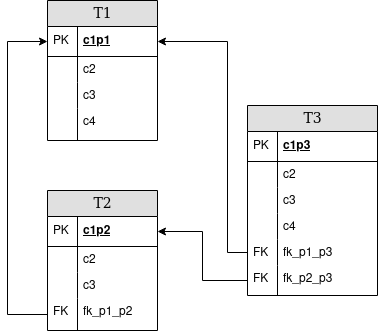
\includegraphics[width=10cm]{images/new_schema.png}
\caption{Adatbázis séma}
\label{fig:new_schema}
\end{figure}

%Az oszlopnevek számozottak. A \texttt{c3}-\texttt{c5} Az értékeik véletlenszerűen generált egészek, \texttt{c3} $in [0, 100]$, \texttt{c4} $in [0, 10000]$, \texttt{c5} $in [0, 10]$.


\SubSection{A táblák feltöltése}

Az adatokat egy \texttt{C++} kóddal generáltam \texttt{.csv} formátumban, ügyelve a kapcsolásokra. Ezeket a táblákat \texttt{MySQLWorkbench} segítségével importáltam.
Egy \texttt{.csv} állomány részlete például az alábbi:
\begin{python}
c1p1, c2, c3, c4
0, 1, 25, 9707
1, 1, 10, 6539
\end{python}

\newpage

\Section{\texttt{EXPLAIN} a gyakorlatban}

A \textit{MySQL Workbench} grafikus képeit fogom használni (melyeket átszerkesztettem a jobb minőség érdekében). Ez a módszer sokkal jobban szemlélteti miképpen dolgozza fel az utasításokat az adatbáziskezelő motorja.

\SubSection{Egyszerű lekérdezés}

Vizsgáljuk a következő lekérdezést:
\begin{python}
SELECT * FROM thesis.T1 WHERE c3 = 25; 
\end{python}
\begin{figure}[h!]
\centering
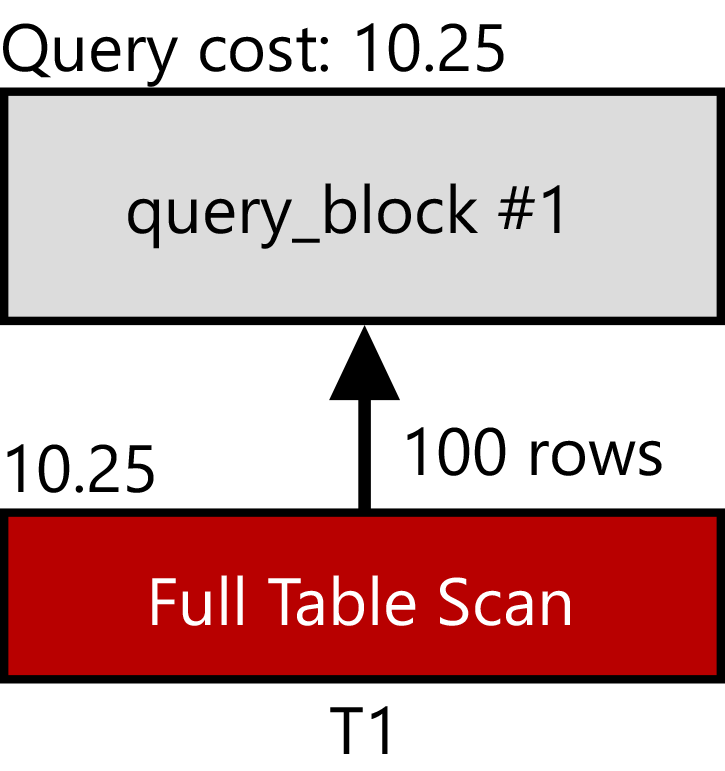
\includegraphics[width=3.5cm]{images/explain/1-1.png}
\caption{Indexelés nélküli lekérdezés}
\label{fig:explain_1_1}
\end{figure}

A program által előállított végrehajtási terven látható (\ref{fig:explain_1_1}. ábra), hogy a \texttt{T1}-es tábla összes sorát át kell vizsgálni a megfelelő értékek megtalálásához. Erre nyújthat megoldást a vizsgált oszlop indexelése, melynek segítségével optimális sebességgel lehet meghatározni az értékek helyét.

Indexek hozzáadása a \texttt{c3} -as oszlophoz:
\begin{python} 
ALTER TABLE thesis.T1 ADD INDEX (c3);
\end{python}

\begin{figure}[h!]
\centering
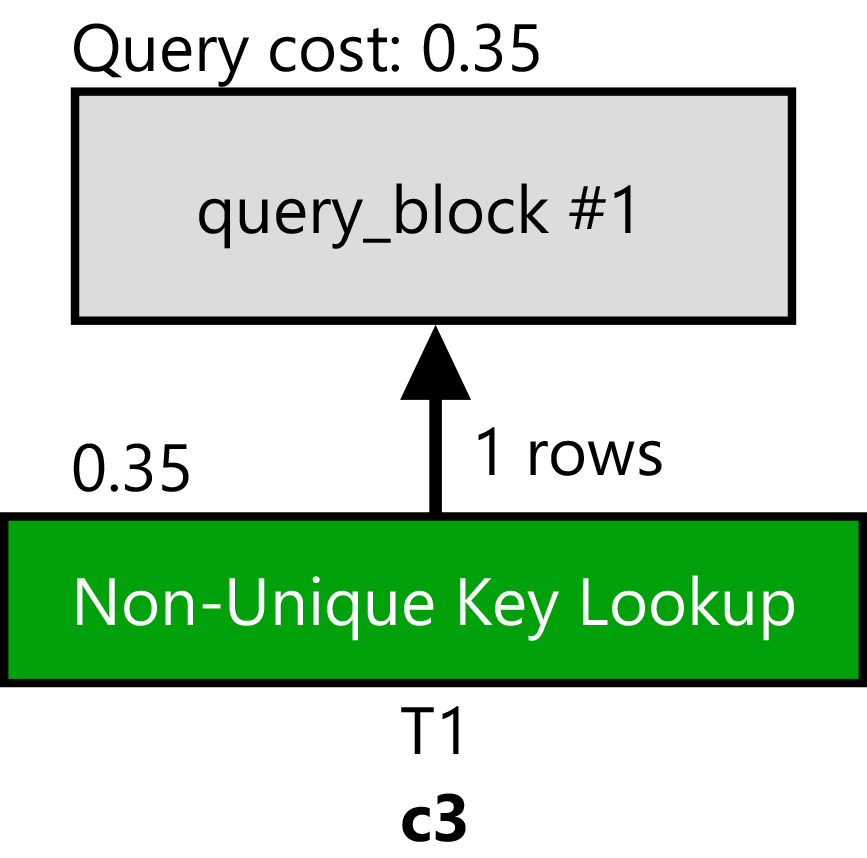
\includegraphics[width=4.2cm]{images/explain/1-2.png}
\caption{Indexelés nélküli lekérdezés}
\label{fig:explain_1_2}
\end{figure}
Újra lefuttatva az előző lekérdezést \aref{fig:explain_1_2}. ábrán láthatjuk, hogy a költsége a töredékére csökkent, melynek az az oka, hogy nem kell minden cella értékét megvizsgálni.

A teljesség kedvéért érdemes megemlíteni, hogy a létrehozott indexet az alábbi paranccsal tudjuk eltávolítani.
\begin{python} 
ALTER TABLE thesis.T1 DROP INDEX c3;
\end{python}

\newpage

\SubSection{Csoportosítás}

Nézzünk meg egy kicsit összetettebb lekérdezést, amelyben már csoportosítás is szerepel.
\begin{python} 
SELECT MAX(c4), c3, c2 FROM thesis.T1 WHERE T1.c3 = 18 GROUP BY c2;
\end{python}

\begin{figure}[h!]
\centering
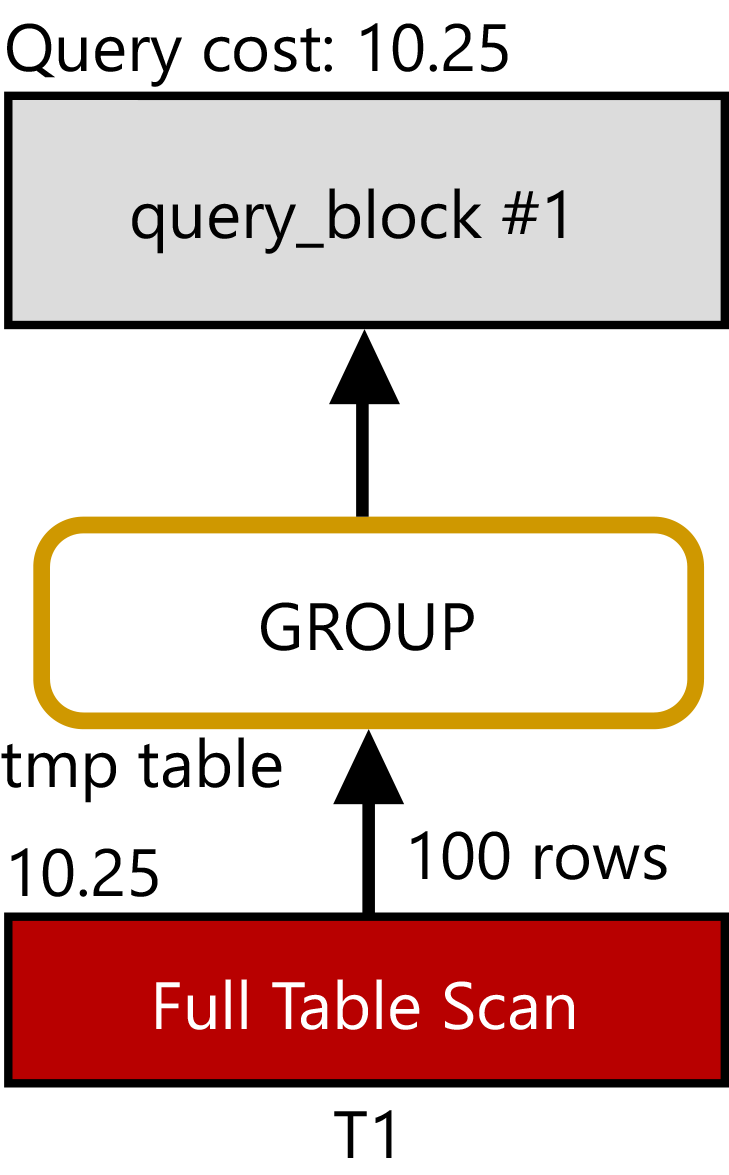
\includegraphics[width=3.5cm]{images/explain/2-1.png}
\caption{Csoportosítás indexelés nélkül}
\label{fig:explain_2_1}
\end{figure}

A lekérdezés elemzésénél két problémát fedezhetünk fel (\ref{fig:explain_2_1}. ábra). Az egyik, hogy a teljes tábla átvizsgálásra kerül, a másik pedig egy ideiglenes tábla létrejötte, ami a lekérdezés idejére memóriát foglal.

\begin{figure}[h!]
\centering
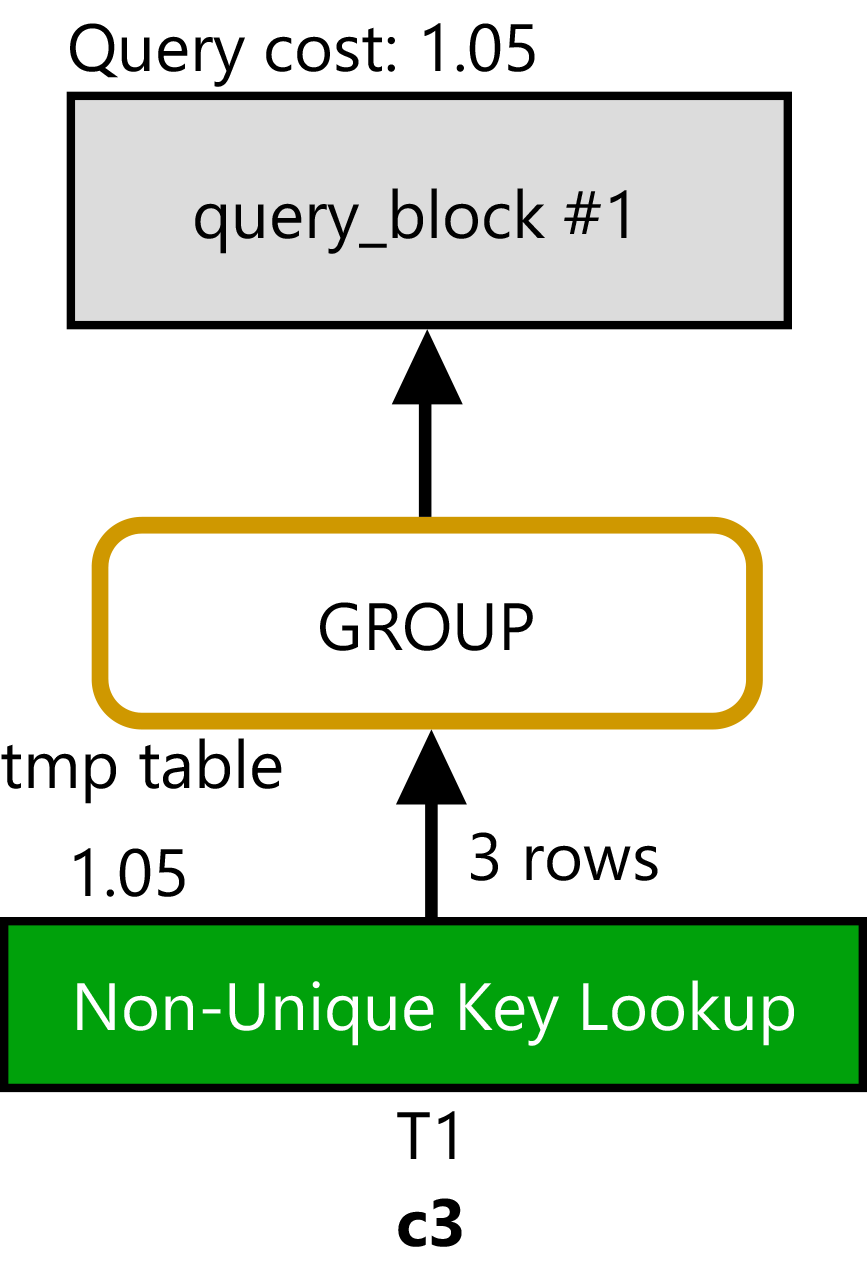
\includegraphics[width=4.2cm]{images/explain/2-4.png}
\hspace{1cm} 
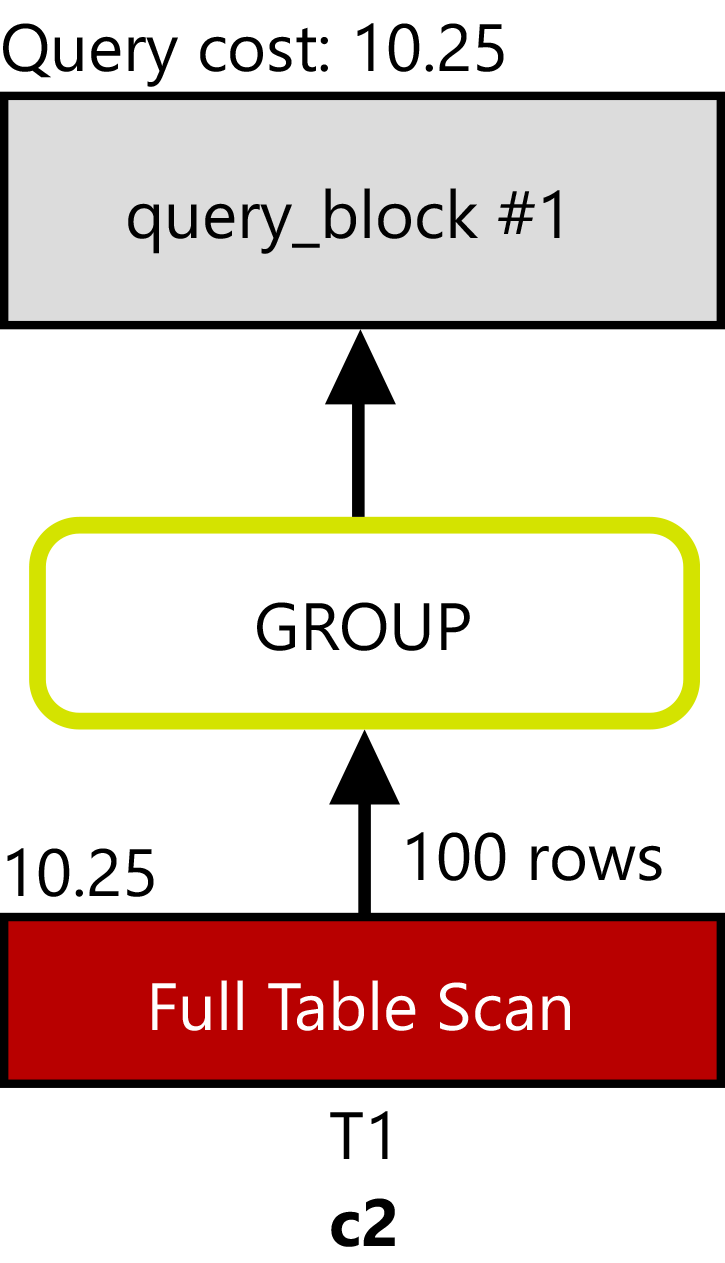
\includegraphics[width=3.51cm]{images/explain/2-2.png}
\hspace{1cm} 
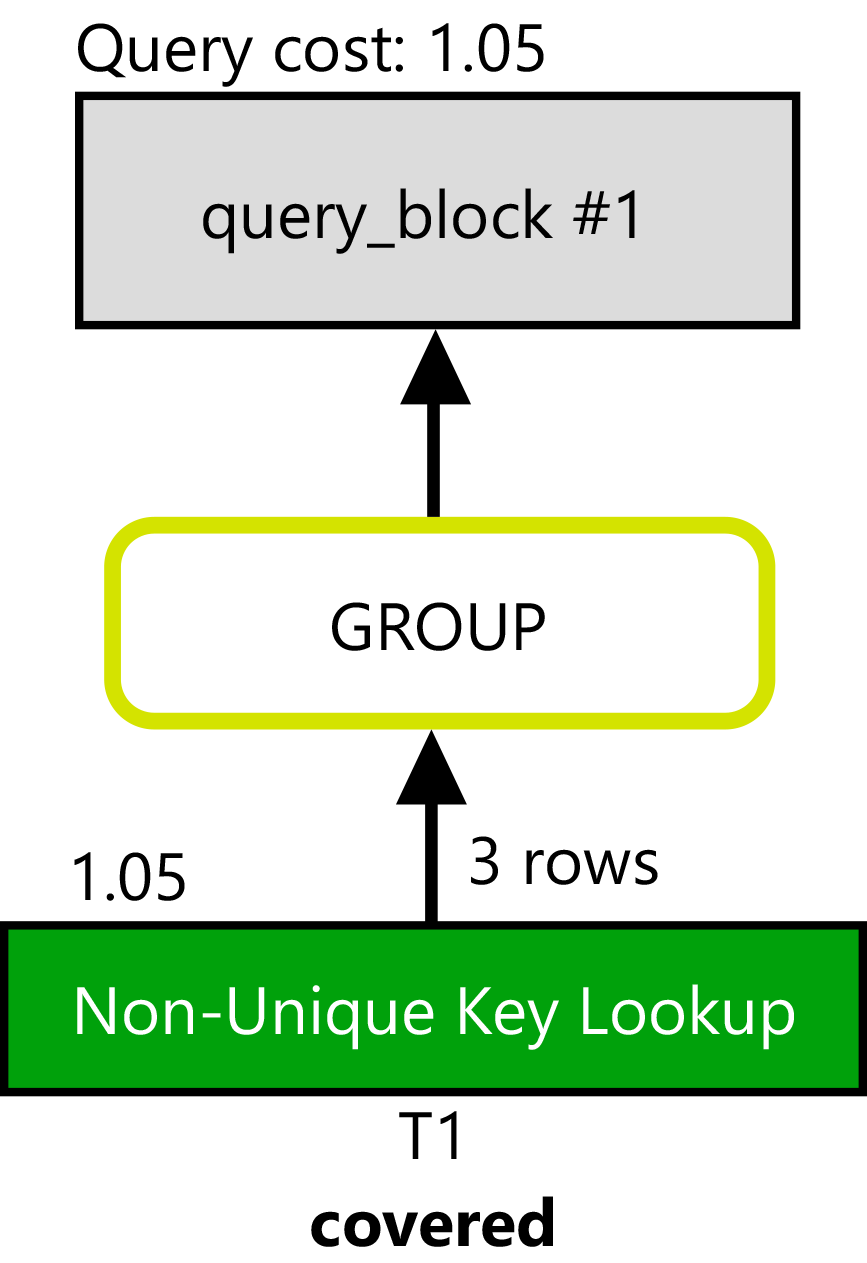
\includegraphics[width=4.2cm]{images/explain/covered.png}
\caption{Indexelések változatai.}
\label{fig:covered}
\end{figure}

Nézzük a következő négy indexelést (\ref{fig:covered}. ábra):
\begin{itemize} 
\item A \texttt{c3}-as oszlop indexelésével az első példához hasonlóan lecsökkent a szűrés költsége.
\item A \texttt{c2}-es oszlop indexelésével az ideiglenes tábla nem jön létre lekérdezés közben.
\item \texttt{c2} és \texttt{c3}-as külön indexelése esetén ugyan az történik mint \texttt{c3} indexelésekor.
\item \texttt{c2} és \texttt{c3} közös indexelésével egyesíthetjük a két előnyt, és így a lekérdezés optimális sebességű és memória igényű lesz.
\end{itemize} 
Kevert index létrehozása és törlése az alábbi SQL lekérdezésekkel valósítható meg:
\begin{python}
ALTER TABLE T1 ADD INDEX covered (c3,c2);
ALTER TABLE thesis.T1 DROP INDEX covered;
\end{python}

\SubSection{Kapcsolt táblák}

Ez a lekérdezés már összetettebb, annak érdekében, hogy látszódjon a lekérdezés optimalizáló mely esetekben, milyen sorrendben kapcsolja össze a táblákat.
\begin{python}
SELECT T1.c3, T2.c2, T3.c3
FROM T3 JOIN T2 JOIN T1 
    ON (T1.c1p1 = T2.fk_p1_p2 AND T2.c1p2 = T3.fk_p2_p3) 
WHERE T3.c4 = 5 AND T1.c2 = 1;
\end{python}

\begin{figure}[h!]
\centering
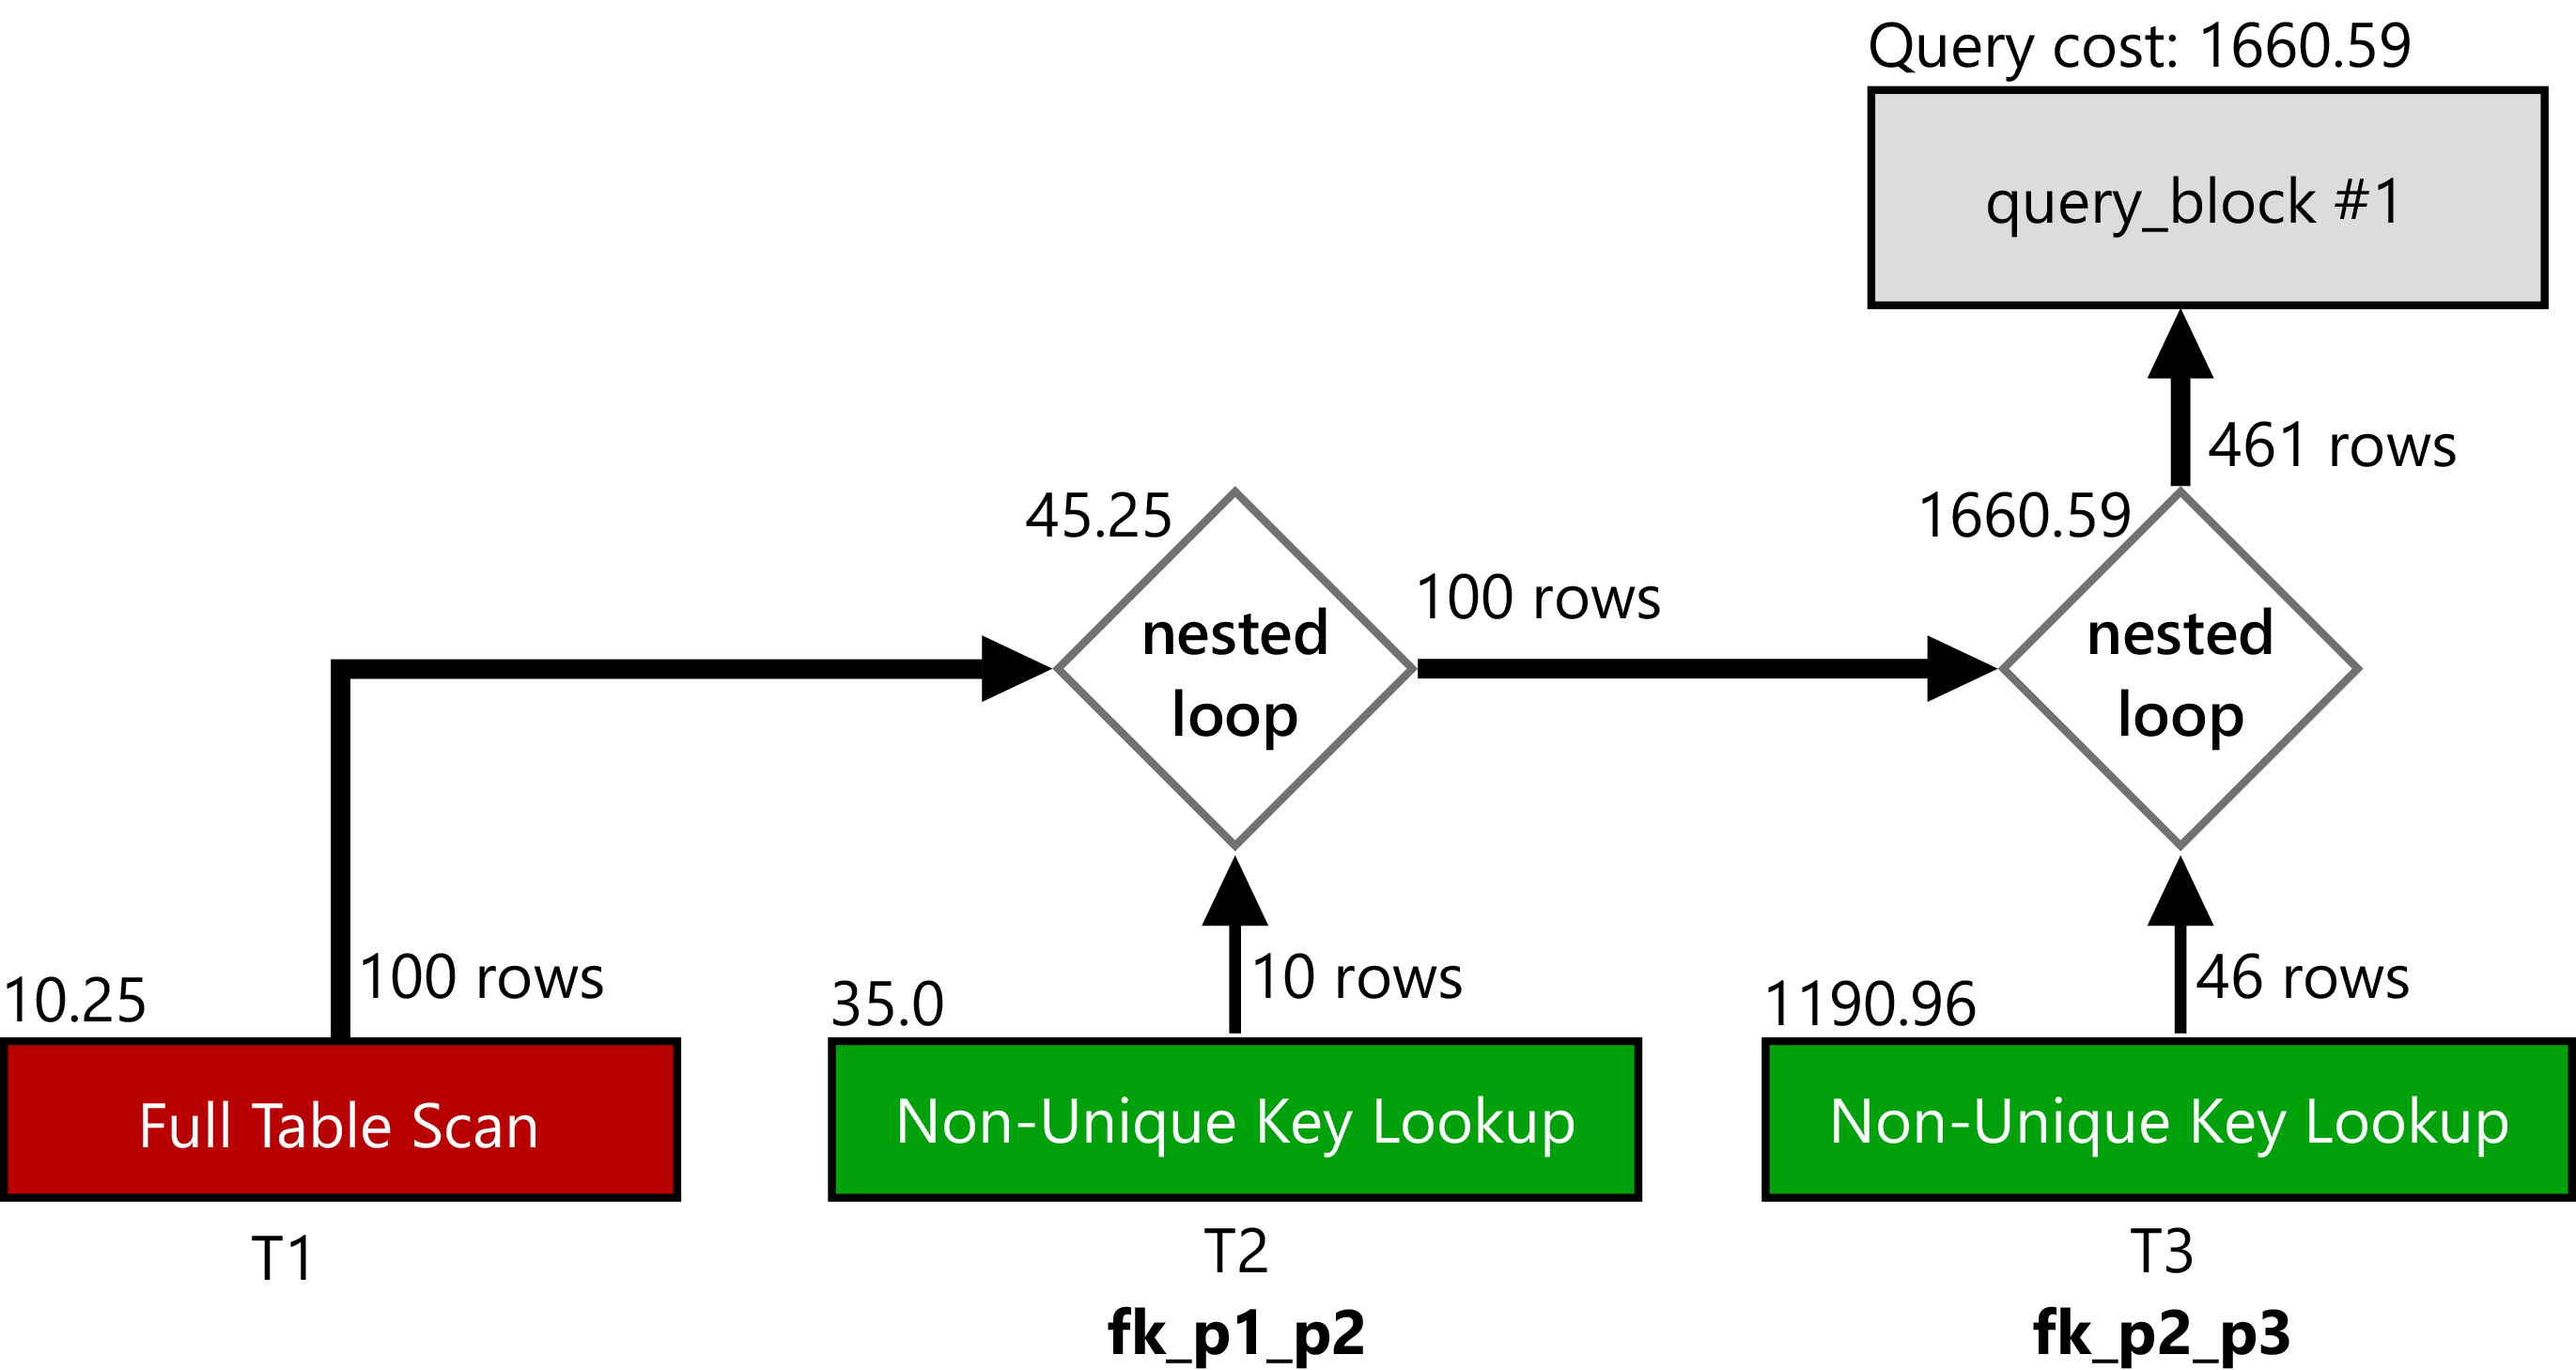
\includegraphics[width=14cm]{images/explain/3-1.png}
\caption{JOIN indexelés nélkül}
\label{fig:explain_3_1}
\end{figure}

Az első észrevétel, hogy a táblák kapcsolási sorrendje nem egyezik a lekérdezésben szereplő sorrenddel, tehát egyszerű \texttt{JOIN} esetében ezzel nem kell törődni. Láthatjuk, hogy a teljes tábla átvizsgálása itt is problémát jelent (\ref{fig:explain_3_1}. ábra). 

Miután a \texttt{T3}-as tábla vizsgált oszlopát indexeléssel láttam el, szinte ugyanezt az eredményt kaptam, leszámítva két értéket. \texttt{T3}-nál a költség 1190.96-ról 1198.86-ra nőtt, illetve a 2. \texttt{nested loop}-nál a sorok száma 450 re csökkent.

\newpage

A következő vizsgálatban csak \texttt{T1} \texttt{c2} -es oszlopa indexelt.

\begin{figure}[h!]
\centering
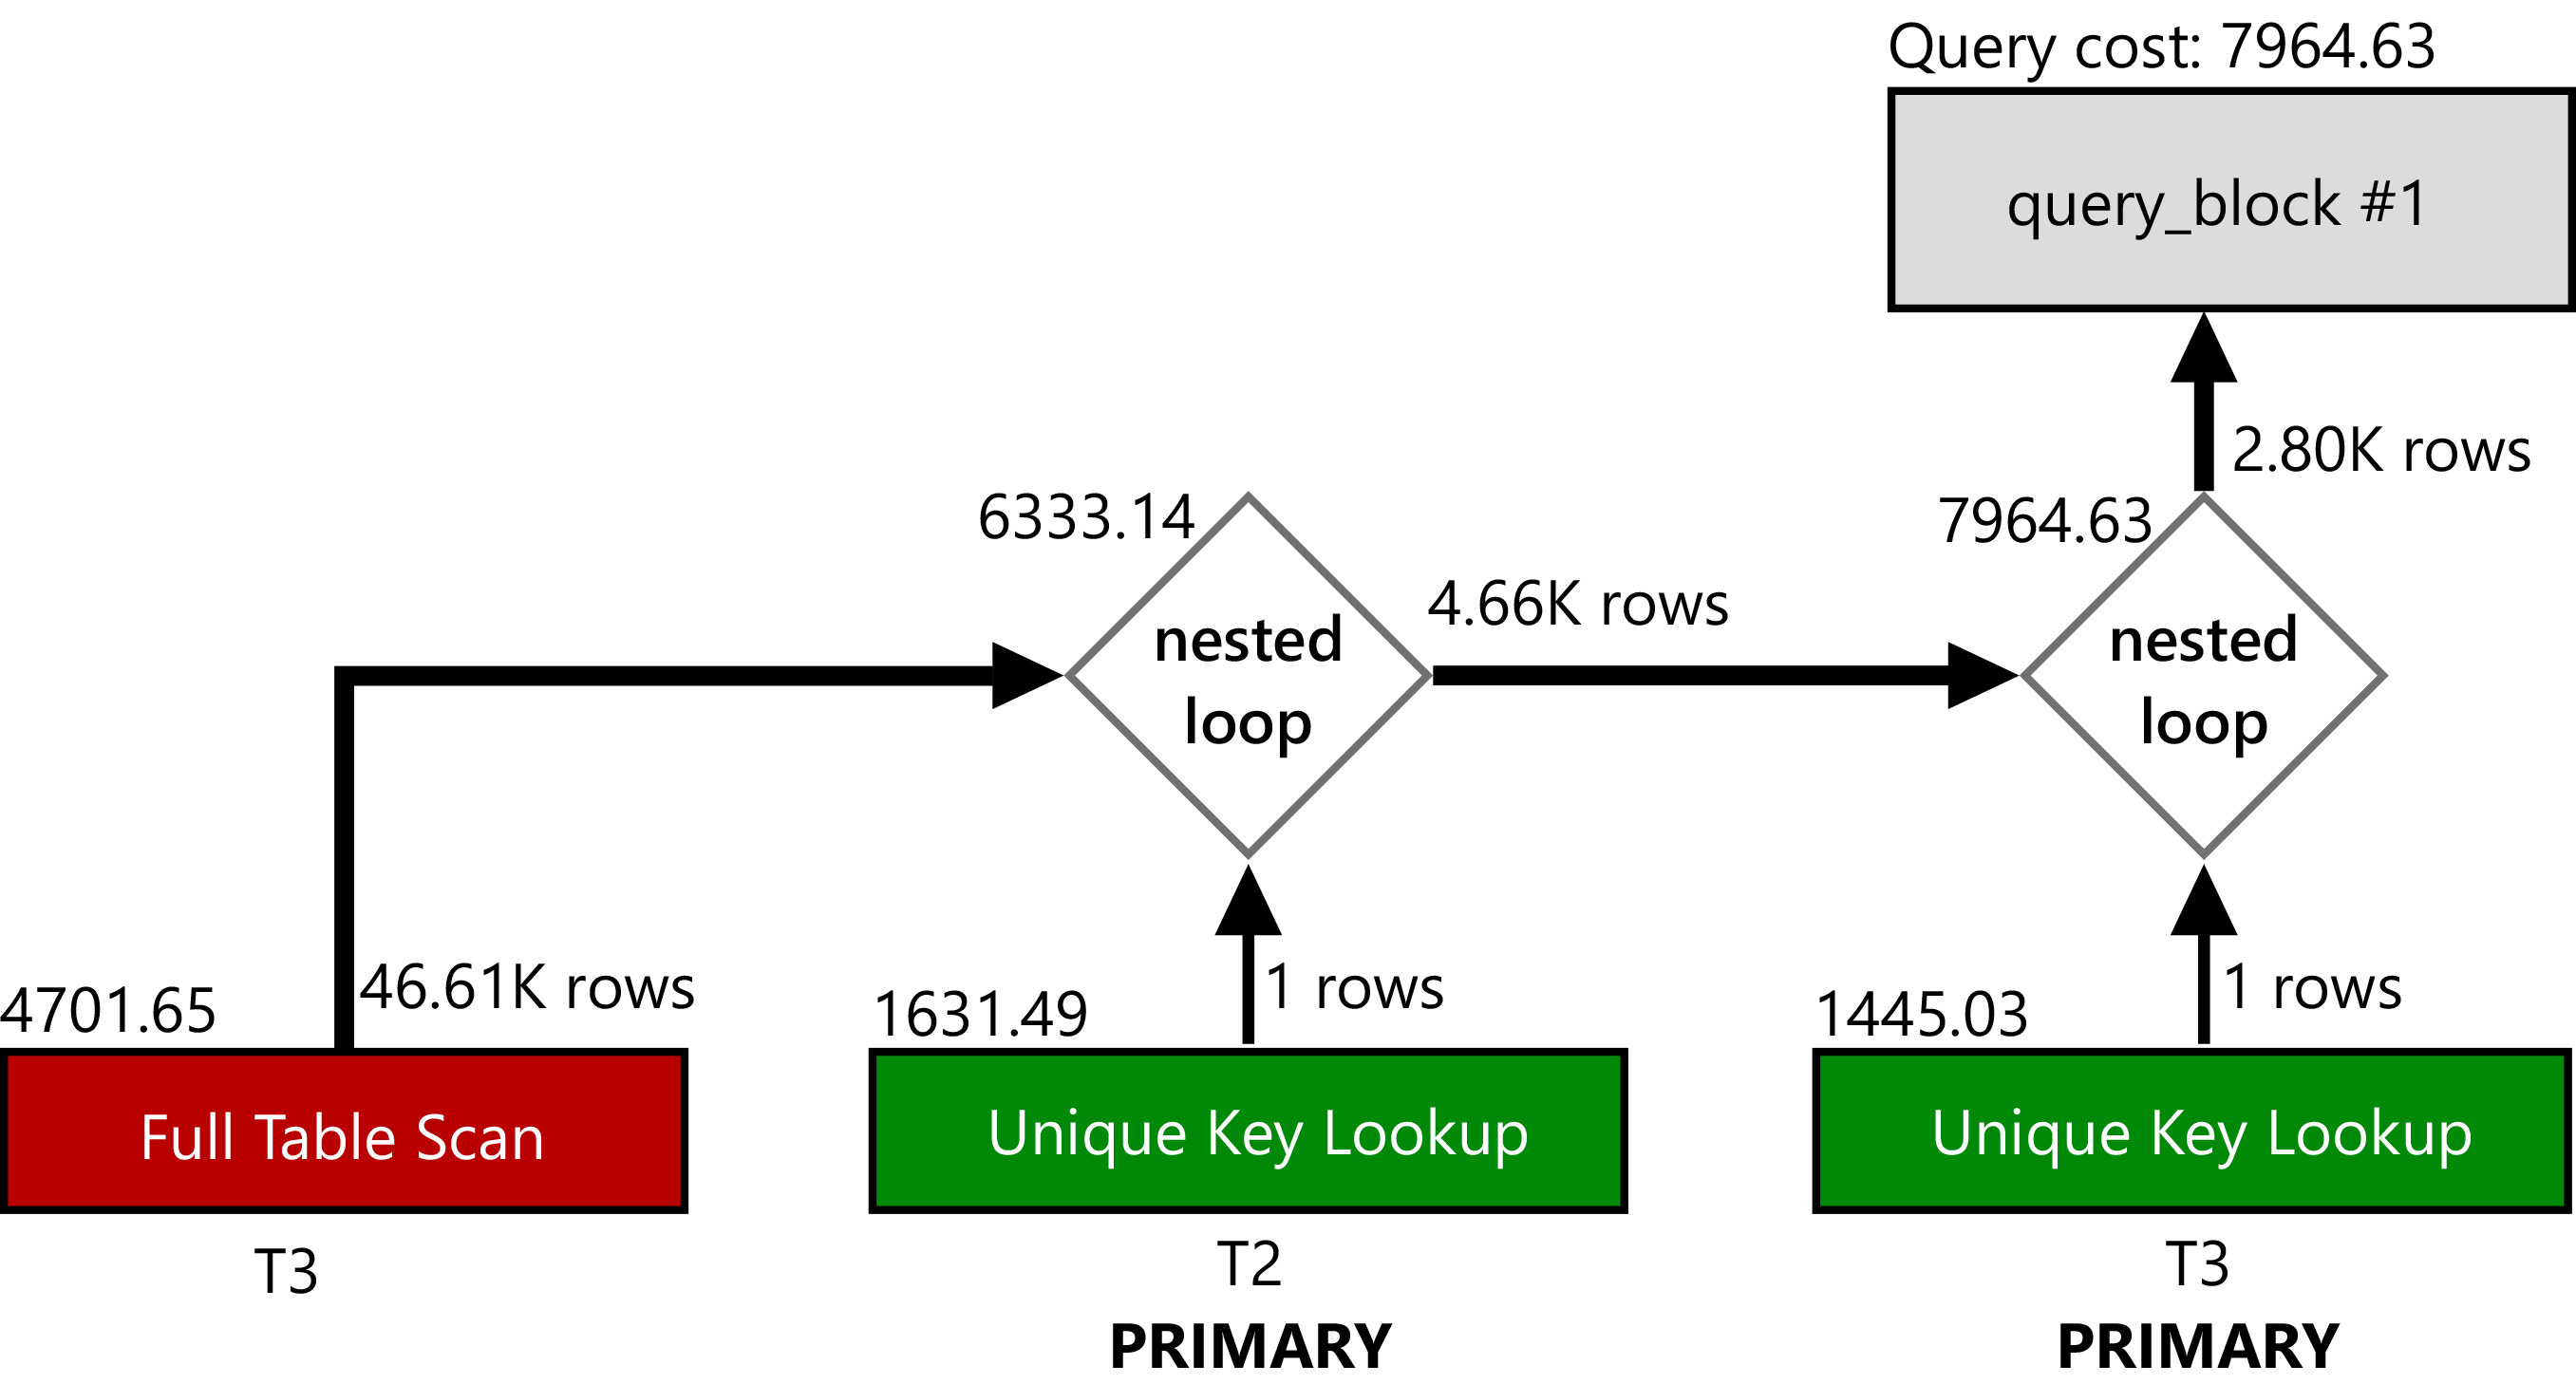
\includegraphics[width=14cm]{images/explain/3-2.png}
\caption{JOIN T1.c2 és T3.c4 indexelésével}
\label{fig:explain_3_2}
\end{figure}

Az eredményből az látszik, hogy megváltozott a táblák kapcsolási sorrendje (\ref{fig:explain_3_2}. ábra). A terv szerint a motor első lépésben szűri a \texttt{T3}-as táblát és csak utána kapcsolja hozzá a többit. A másik dolog amit meg lehet figyelni, hogy nem az idegen kulcs szerepel a használt indexnél, hanem az elsődleges, ez a sorrend változás következménye.

A negyedik vizsgálatban mind a két tábla használt oszlopát indexekkel láttam el.

\begin{figure}[h!]
\centering
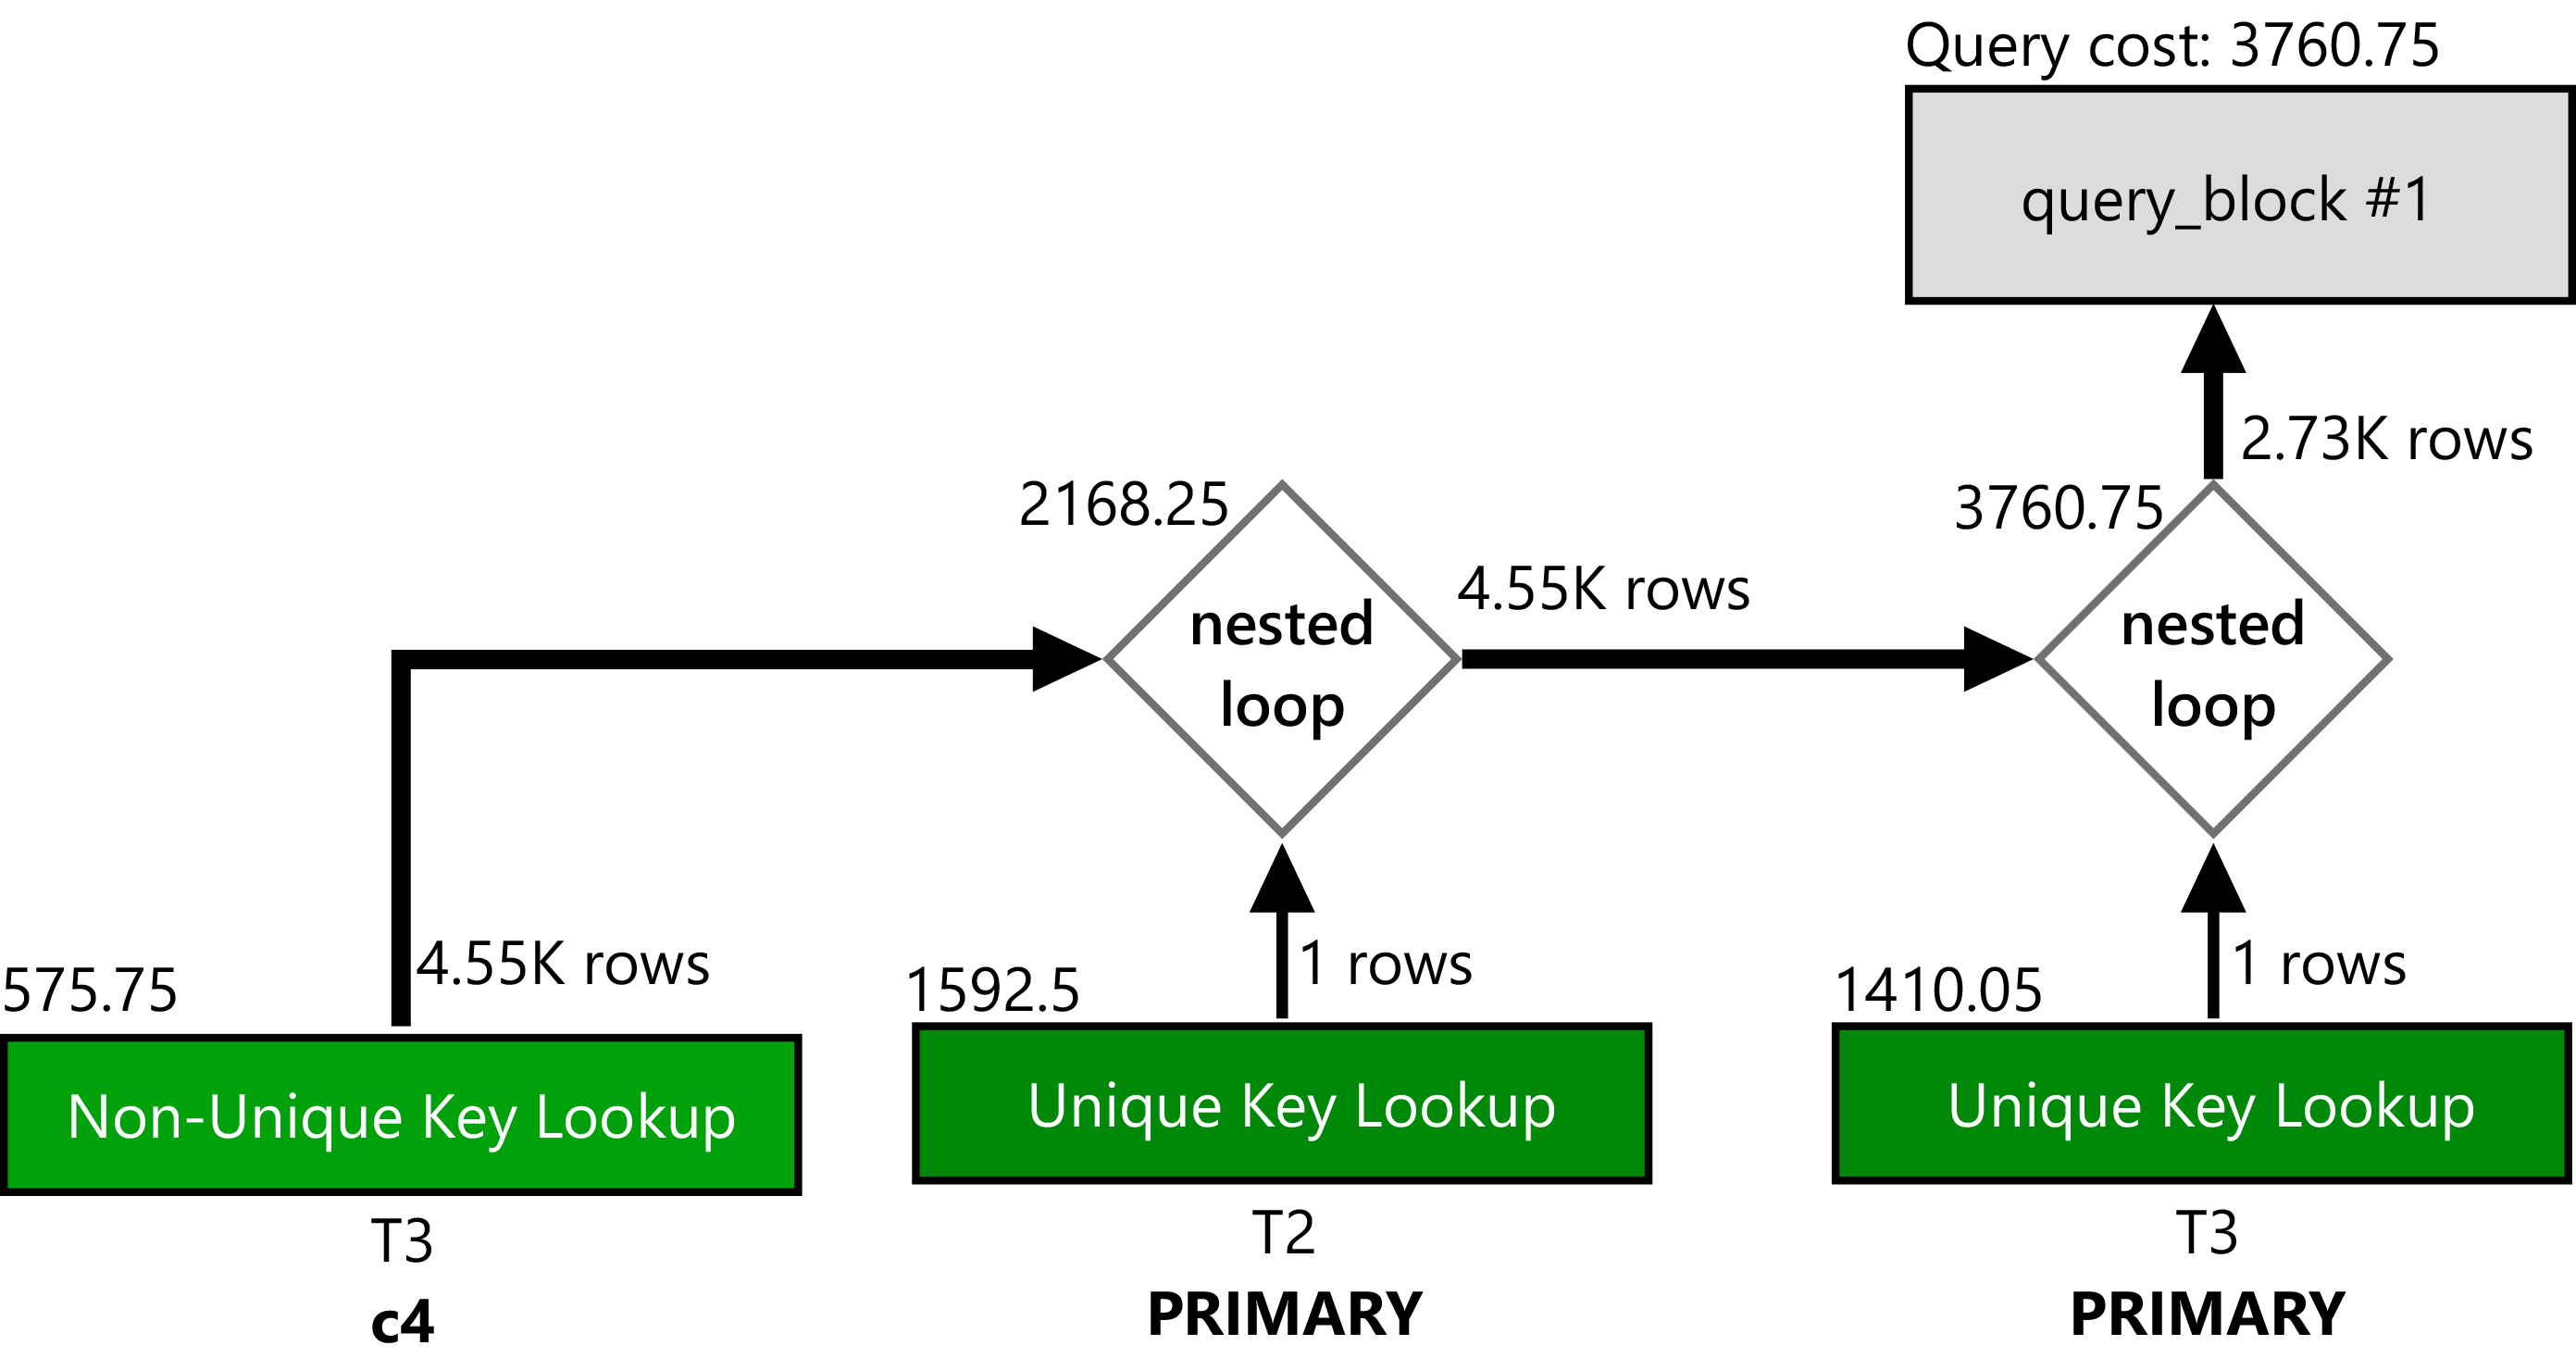
\includegraphics[width=14cm]{images/explain/3-3.png}
\caption{JOIN T1.c2 indexelésével}
\label{fig:explain_3_3}
\end{figure}

\Aref{fig:explain_3_3}. ábrán azt vehetjük észre, hogy a \texttt{T3}-as táblánál is használatban vannak az indexek, így már sebesség optimális a lekérdezés.

Az ábrákon látható \texttt{query cost} megtévesztő lehet, hisz arra enged következtetni, hogy nem érdemes indexelést használni ebben az esetben, viszont a lekérdezés sebességének vizsgálata egyértelműen mutatja, hogy az indexek használata jelentős sebesség növekedéssel járt. 

\Chapter{Saját kód elhelyezése}

Az adatbázis lekérdezések optimalizálása kapcsán felvetődik a kérdés, hogy az optimalizálást pontosan hol lehet és hol érdemes elvégezni. A fejezet ennek a lehetőségeit vizsgálja meg, közvetlenül az adatbázis forráskódjában való elhelyezéssel, és egy saját \textit{Connector Proxy} bemutatásával.

\Section{A \texttt{MySQL} adatbázis fordítása és telepítése}

A \texttt{MySQL} forráskódból való fordítását egy frissen telepített és naprakészre frissített Manjaro 20.2.1-es GNU/Linux disztribúción végeztem el. Telepítés során \textit{non-free} grafikus drivert választottam.
A forrásállomány bárki számára elérhető, és a következő paranccsal klónozható:
\begin{python}
$ git clone https://github.com/mysql/mysql-server.git
\end{python}%$
A fordítás sikerességéhez rendszerenként eltérő csomagok telepítésére lehet szükség. Jelen esetben a következők telepítéseket igényelte a folyamat.
% QUEST: Miért snap-es csomaggal lett telepítve?
% ANSWER: A cmake telepítése a gyártó hivatalos weboldalán található Manjato rendszerhez készült segédlet alapján lett elvégezve.
\begin{python}
 $ sudo snap install cmake --classic
 $ sudo pacman -S rpcsvc-proto
 $ sudo pacman -S pkgconfig
 $ sudo pacman -S make
 $ sudo pacman -S gcc
 $ sudo pacman -S bison
\end{python}%$
%A \textit{Boost} függvénykönyvtár később kapcsoló használatával letölthető.
A következő lépés a \texttt{CMake} futtatása. Ehhez célszerű létrehozni egy mappát ahová az új állományok létrejöhetnek. Ezt nem kötelező megtenni, a forrás könyvtárban is ki lehet adni a parancsot, ehhez a \texttt{CMake} meg fogja adni a szükséges kapcsolót, illetve figyelmeztet arra, hogy nem ajánlatos.
\begin{python}
$ mkdir build
\end{python}%$
Amint ez kész, a forrás mappájában futtathatjuk a következő parancsot:
\begin{python}
$ cmake ./ ../build -DDOWNLOAD_BOOST=1 -DWITH_BOOST=../boost/
\end{python}%$
A megadott kapcsolóval a \textit{Boost} könyvtár letöltődik a megadott helyre, és a \texttt{CMake} regisztrálja ezt. Ha a generátor hibába ütközik, a szükséges csomagokat telepíteni kell, és a \texttt{CMakeCache.txt} fájlt törtölni. Ezek után a \texttt{CMake} újra futtatható, de már a \textit{Boost}-hoz tartozó kapcsolók nélkül.

A sikeres futás jelzi, hogy minden készen áll a fordításra, nincs hiányzó csomag.
A \texttt{make} parancs futtatása következik. Ez egy hosszú folyamat, jelen konfiguráción 120 percet vett igénybe. 

A sikeres fordítást követően létre kell hoznunk egy \texttt{data} mappát a szerver számára.
\begin{python}
$ mkdir data
\end{python}%$
Az első futtatást rendszergazdaként a megadott kapcsolóval kell végrehajtani, csak ekkor tudja a szerver létrehozni a fájljait.
\begin{python}
$ sudo ./bin/mysqld --initialize
\end{python}%$
Ekkor kapunk egy jelszót a szerverre való csatlakozáshoz. Következő futtatás előtt szükség lehet a \texttt{data} mappa jogosultságainak állítására, különben a szerver a normál indítás során nem tudja inicializálni az \textit{InnoDB}-t olvasási hiba miatt.
\begin{python}
$ sudo chmod -R 777 ./data
\end{python}%$
Ezután futtathatjuk a szervert a
\texttt{./bin/mysqld} paranccsal, vagy telepíthetjük is azt a \texttt{make install} paranccsal.

A szerverre csatlakozni a következő paranccsal tudunk.
\begin{python}
$ ./bin/mysql -u root -p
\end{python}%$
A generált jelszó bemásolásával belépünk, majd megváltoztatjuk azt.
\begin{python}
ALTER USER 'root'@'localhost' IDENTIFIED BY 'uj jelszo';
\end{python}
Használhatjuk a \texttt{MySQL Workbench}-et is, ami első belépéskor megkér minket a módosításra.
% TODO: SQL-es környezetet lesz majd célszerű használni helyette!

\Section{A \texttt{MySQL} Connector}

A \texttt{Connector} \textit{MySQL} alapszabványú \textit{driver}-eket biztosít különböző nyelveken, amelyek lehetővé teszik a fejlesztők számára, hogy adatbázis alkalmazásokat írjanak a támogatott nyelveken \cite{connector}. Ezen kívül egy natív \textit{C} könyvtár teszi lehetővé azt, hogy a \textit{MySQL}-t közvetlenül beágyazhassák alkalmazásaikba.
A következő \texttt{MySQL} által fejlesztett driver\-ek érhetőek el:
\begin{itemize}
	\item \texttt{ADO.NET}, \texttt{ODBC}, \texttt{JDBC}, \texttt{Node.js}, \texttt{Python}, \texttt{C++}, \texttt{C} és \texttt{C API} a klienshez,
\end{itemize}
az alábbiakat pedig a \texttt{MySQL} közössége fejleszti:
\begin{itemize}
	\item \texttt{PHP}, \texttt{Perl}, \texttt{Ruby}, \texttt{C++ Wrapper}.
\end{itemize}

\SubSection{A Connector/C++ használata}

Az állományok letölthetőek a készítő hivatalos weboldaláról (\url{https://dev.mysql.com/downloads/connector/cpp/}) a következő változatokban:
\begin{itemize}
	\item Linux - Generic,
	\item All,
	\item Linux - Generic (glibc 2.12) (x86, 64-bit), Compressed TAR Archive.
\end{itemize}
Ezt a letöltés után kicsomagoljuk. A tartalma egy \texttt{include} és egy \texttt{lib64} mappa. Az \texttt{include} mappa tartalmát a \texttt{usr/include} könyvtárba másoljuk, a \texttt{lib64}-ét pedig az \texttt{usr/lib64} mappába.

Ezután szükség lesz egy külön felhasználóra amellyel a program csatlakozni fog a szerverünkre. Ezt létrehozhatjuk a \texttt{Workbench} alkalmazásban is.
\begin{python}
CREATE USER 'newuser'@'localhost' IDENTIFIED BY 'password';
\end{python}

\SubSection{Első program}

Kipróbálni például a dolgozathoz mellékelt \texttt{mysql\_speed} mappában lévő programmal lehetséges.
 
A \texttt{Connector} használatához a következő osztályok létrehozása szükséges \cite{connector_program}:
\begin{cpp}
sql::Driver *driver;
sql::Connection *con;
sql::Statement *stmt;
sql::ResultSet *res;
sql::PreparedStatement *pstmt;
\end{cpp}
A szerverhez csatlakozni és az adatbázist kiválasztani a következő formában tudjuk.
\begin{cpp}
driver = get_driver_instance();
con = driver->connect("tcp://192.168.0.43:3306", "program", "a");
con->setSchema("thesis");
\end{cpp}
A következő két sor maga a lekérdezés. Az első utasítás elkészíti a szövegből a szerver számára is értelmezhető utasítást, a második sor pedig elküldi azt a szervernek és megvárja a választ:
\begin{cpp}
pstmt = con->prepareStatement("SELECT * FROM T3");
res = pstmt->executeQuery();
\end{cpp}

Az eredményt a \texttt{res} objektumon végig lépkedve tudjuk kiolvasni, a lekért oszlop nevének megadásával és a típusnak megfelelő \texttt{get} függvénynél.
\begin{cpp}
while (res->next())
cout << res->getInt("c1p3") << "\t" << res->getInt("c2") << "\t"
<< res->getInt("c3") << "\t" << res->getInt("c4") << "\t"
<< res->getInt("fk_p1_p3") << "\t" << res->getInt("fk_p2_p3") 
<< endl;
\end{cpp}
Lekérdezés után fontos törölni az eredményhalmazt és az elkészített utasítást, ugyanis ezek memóriát foglalnak, és több lekérdezés esetén megtelhet akár a teljes memória is.
\begin{cpp}
delete res;
delete pstmt;
\end{cpp}
Futtatáshoz és fordításhoz a következő parancsokat használhatjuk: 
\begin{python}
$ g++ -D_GLIBCXX_USE_CXX11_ABI=0 connectortest.cpp 
-o connectortest.out -lmysqlcppconn
$ ./connectortest.out
\end{python}

\Section{Connector proxy létrehozása}

Azt feltételezhetjük, hogy a rendelkezésre álló \texttt{MySQL} elérési felületet érdemes megtartani valamilyen formában a lekérdezések optimalizálása során. Ez többek között az alábbiakkal indokolható.
\begin{itemize}
	\item A felület jól átgondolt, a területen járatos szakemberek készítették, és a használat szempontjából kiállta az idő próbáját.
	\item Elterjedt. Amennyiben az a cél, hogy az elkészített szoftver előnyeit minél többen használni tudják, és akarják is, arra kell törekedni, hogy az új felhasználóknak minél kevesebb plusz munkát jelentsen az elsajátítása.
	\item Lehetőséget ad, hogy egy saját implementációval transzparens módon megoldható legyen az optimalizálás. Ez olyan szempontból kifejezetten praktikus, hogy így opcionálissá tehető az optimalizálási módszer használata. A szokványos és a dolgozatban bemutatásra kerülő \texttt{OpenCL}-el optimalizált elérés között a váltás kényelmesen megtehető.
\end{itemize}

A \textit{proxy} nevű tervezési minta kiválóan alkalmas lehet az említett feladat megoldására. \Aref{fig:proxy_arch}. ábrán bal oldal láthatjuk a hagyományos módszert, ahogy az adatokhoz hozzá lehet férni egy alkalmazásból. A jobb oldalt a proxy segítségével optimalizált változat látható.

\begin{figure}[h!]
\centering
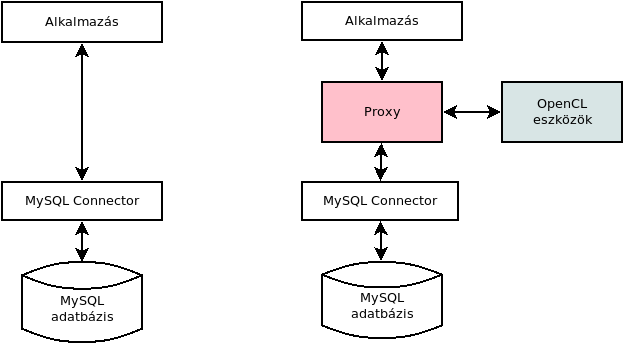
\includegraphics[width=\textwidth]{images/proxy_arch.png}
\caption{A hagyományos és az optimalizáláshoz használt proxy-val kiegészített felépítés}
\label{fig:proxy_arch}
\end{figure}

A feldolgozási folyamatot \aref{fig:process}. ábrán látható formában képzelhetjük el.

\begin{figure}[h!]
\centering
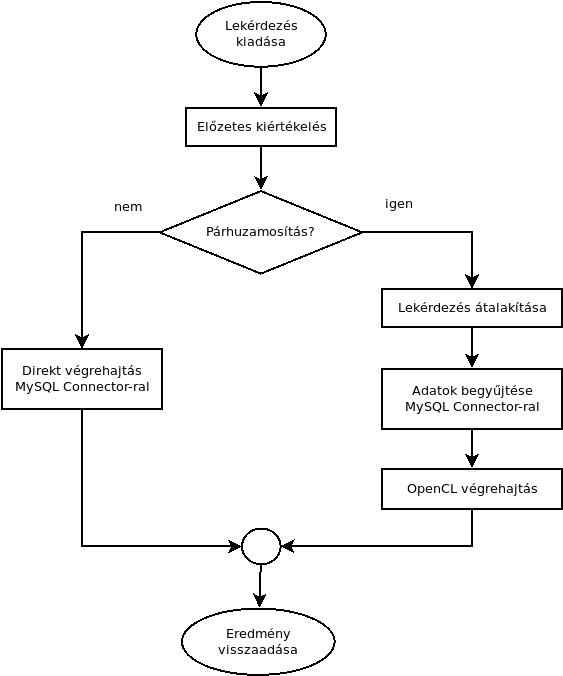
\includegraphics[width=\textwidth]{images/process.png}
\caption{A feldolgozási lépések a proxy beiktatásával}
\label{fig:process}
\end{figure}

Ennek az egyik igen fontos eleme az előzetes kiértékelő, amely a kapott lekérdezésről meg tudja állapítani, hogy azt érdemes-e párhuzamosítani.
\begin{itemize}
	\item Mivel ennek egy gyors döntést kell hoznia, a lekérdezést nem fogja végrehajtani, ezért csak egy becslést ad arra, hogy melyik végrehajtási mód lehet megfelelő.
	\item A kimenete egyszerűen csak egy logikai érték.
	\item Figyelembe kell vennie a lekérdezés összetettségét, az aktuálisan rendelkezésre álló számítási kapacitásokat, és adatbázisban lévő adatok mennyiségét.
	\item Lehetőséget adhatunk a felhasználónak, hogy direkt módon döntsön a feldolgozás menetéről. Ha a felhasználó ismeri a rendszer előnyeit, hátrányait olykor könnyedén dönthet arról, hogy használja-e az \texttt{OpenCL}-es kiértékelést. Például ha sok visszatérő sorra számít akkor használja, ha nem biztos, akkor automatikus módban hagyja.
\end{itemize}

A következő fontos elem a lekérdezés átalakítása, amely a lekérdezést szétválasztja adatgyűjtési és kiértékelési részekre.
\begin{itemize}
	\item A párhuzamos végrehajtásnál úgy általában azt feltételezzük, hogy szelekciós műveletről van szó.
	\item Az adatgyűjtést követően már a számítási rész végrehajtásához nem szükséges az adatbázishoz fordulni.
\end{itemize}

Érdekes lehet egy olyan változatot is felvetni, amelyben a lekérdezés egyidejűleg elindul a direkt végrehajtás és a párhuzamos végrehajtás irányába is, majd azt az eredményt szolgáltatja, amelyik hamarabb visszatér. Ez elvi szinten ugyan megoldható, viszont feltételezhetően a konkurens végrehajtás miatt mindkét számítási idő sérülni fog az erőforráslimitek miatt. A későbbiekben tehát az előzetes kiértékelés eredményére hagyatkozhatunk.

\SubSection{Az API illesztése}

A dolgozat keretein belül nem cél a teljes \texttt{Connector} interfész megvalósítása, csak annak egy részhalmaza. Mivel proxy-ról van szó, ezért az összes olyan művelet átkötése mennyiségi problémát jelent csak, amely nem változtatja meg a végrehajtás módját.

A driver beállítások és az adatbázishoz kapcsolódás változatlan kell legyen, mivel azok szükségesek ahhoz, hogy hozzáférjünk az adatbázishoz.

A különbség a \texttt{prepareStatement} kapcsán jelenik meg. Ehhez kell tehát egy saját implementációt adni, amelyik kompatibilitási okokból származhat közvetlenül az \texttt{sql::PreparedStatement} osztályból. Hogyha azt szeretnénk, hogy a kódban csak az \texttt{include}-okat kelljen megváltoztatni, akkor érdemes a \texttt{Driver} és \texttt{Connection} osztályokat szintén származtatni. Mivel az interfész megtartható, ezért statikus linkeléssel is lehetőség adódhat a funkció cseréjére, vagyis hogy a fejlesztő (mint célfelhasználó) a saját alkalmazásához nem a \texttt{Connector}-t fogja használni, hanem a proxy-t (amely aztán használja a \texttt{Connector}-t).



\Chapter{Az \texttt{OpenCL} nyelv}

Open Computing Language egy keretrendszer amely lehetőséget ad olyan programok írására amelyek különböző platformokon is futtathatóak.
Az \texttt{OpenCL} meghatároz egy programozási nyelvet az eszközök és API-k számára a platformok vezérléséhez és a számítások végrehajtásához az eszközökön. Szabványos interfészt biztosít a párhuzamos számításokhoz, melyekhez adatalapú és feladatalapú párhuzamosítást használ.

Fontos észrevenni, hogy az \texttt{OpenCL} natív módon képes beszélni az eszközök nagy részével, de ez nem azt jelenti, hogy a kód optimálisan fog futni. Ugyanis különböző \texttt{CL} eszközök különböző funkciókkal vannak ellátva. Gyártó specifikus kiterjesztések elkerülésével a kód hordozható lesz, de nem sebesség optimális.

\begin{figure}[h!]
\centering
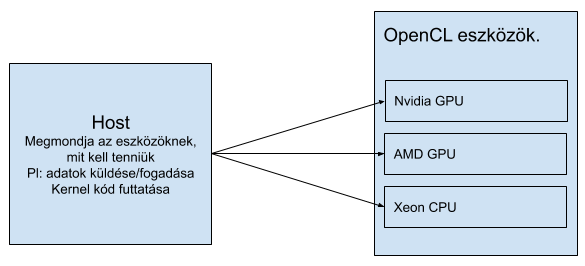
\includegraphics[width=\textwidth]{images/opencl.png}
\caption{\texttt{OpenCL}}
\label{fig:opencl}
\end{figure}

A következő esetekben a GPU-t érdemes használni:
\begin{itemize}
\item Gyors permutáció: Az eszközök gyorsabban mozgatáják a memóriát mint a Host.
\item Adat átváltás: Egyik formátumról másikra.
\item Numerikus gyorsítás: Az eszközök gyorsabban számolnak nagyobb adatdarabokkal mint a Host.
\end{itemize}
Jelen esetben a Host egy asztali számítógép.
Számítási eszközei: CPU, GPU, FPGA, DSP.
A számítási egységek: a magok száma
Elemek feldolgozása: ALU magonként.

\texttt{OpenCL} használata mellett szükségtelen gondolkozni azon, hogy pontosan mi is végzi el a számításokat. Ugyanis az \texttt{OpenCL} modelljének illeszkedése egy adott hardverhez, a gyártók feladata.

\begin{table}[h!]
\centering
\caption{CPU-k és GPU-k összehasonlítása}
\medskip
\label{tab:cpuvsgpu}
\begin{tabular}{|p{7cm}|p{7cm}|}
\hline
Alacsony számítási sűrűség & Magas számítási sűrűség \\
\hline
Komplex logikai vezérlő & Magas számítási és memória-hozzáférés \\
\hline
Nagy caches & Nincs nagyméretű gyorsítótár  \\
\hline
Optimalizált a soros műveletekre.
\begin{itemize}
	\item Kevesebb végrehajtási egység (ALU).
	\item Magas órajel sebesség.
\end{itemize} & Beépített párhuzamos műveletek.
\begin{itemize}
	\item Sok párhuzamos végrehajtási egység (ALU).
	\item A grafika a párhuzamosság legismertebb esete.
\end{itemize} \\
\hline
Keskeny adatvezeték <30 szakasz & Széles adatvezeték több száz szakasz \\
\hline
Alacsony késleltetési tolerancia & Magas áteresztőképesség, magas késleltetési tolerancia \\
\hline
Az újabb CPU-k több párhuzamosításra képesek & Újabb GPU-k
\begin{itemize}
	\item Jobb áramlást vezérlő logika
	\item Scatter/Gather Memory Access
	\item Már nem egyirányúak a pipeline-ok
\end{itemize} \\
\hline
\end{tabular}
\end{table}

\Section{Az OpenCL elemei}

\SubSection{Eszköz modell}

\begin{figure}[h!]
\centering
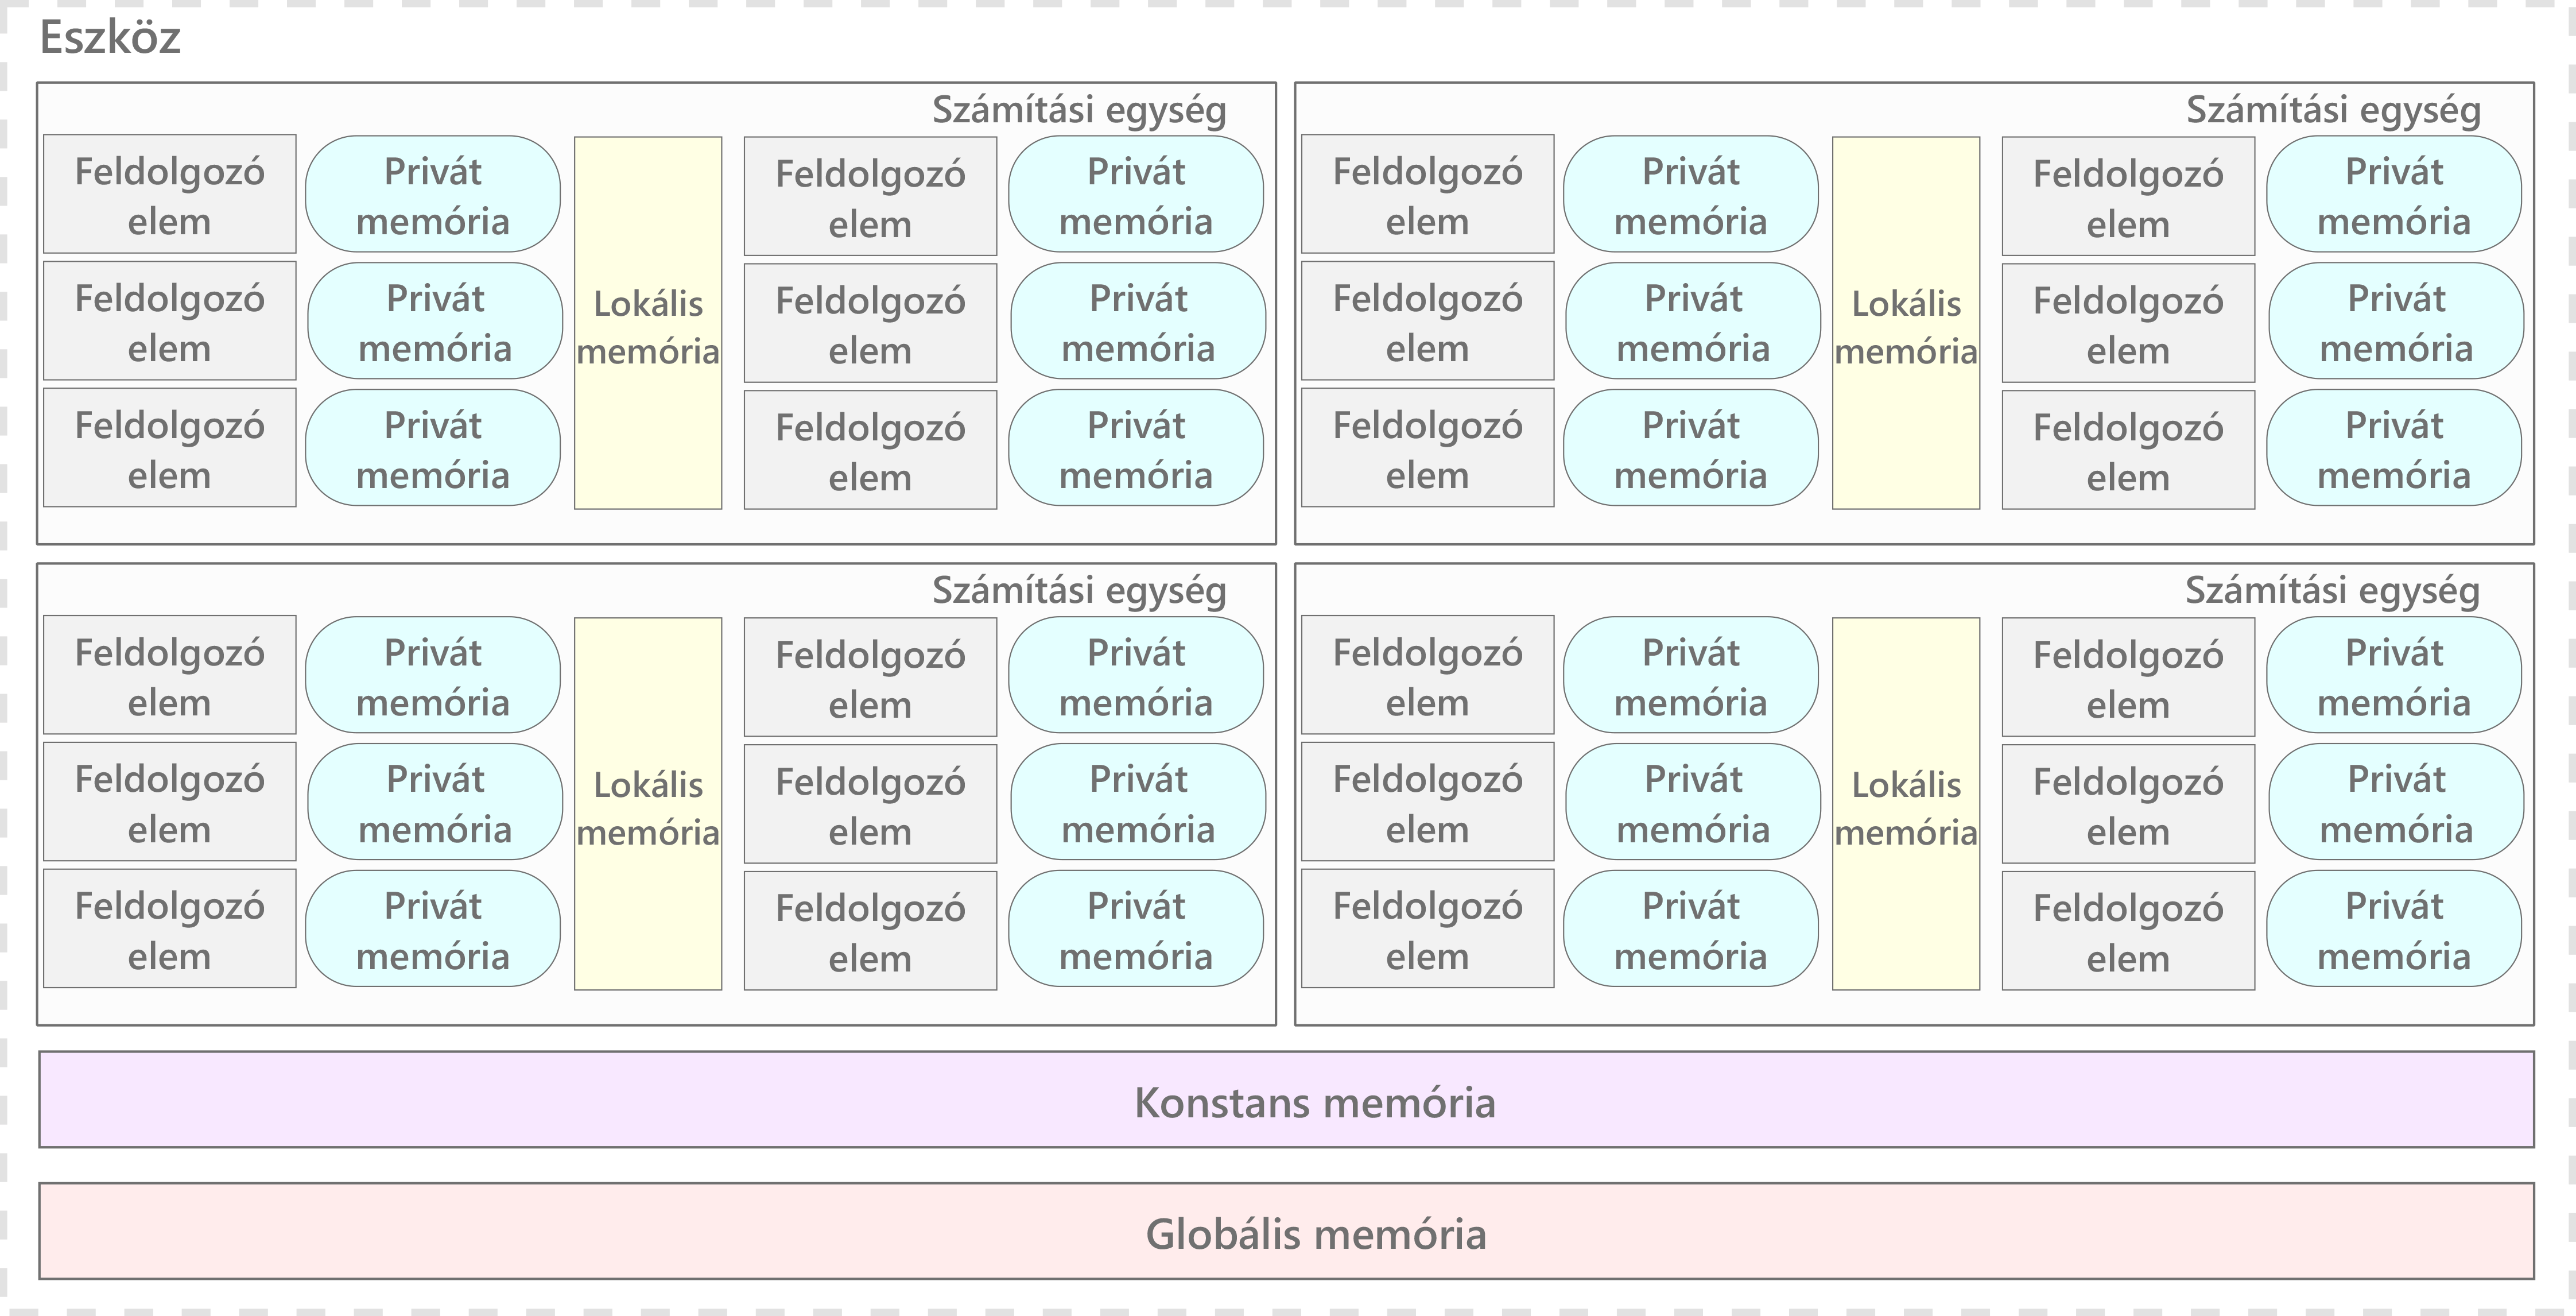
\includegraphics[width=\textwidth]{images/device.png}
\caption{\texttt{OpenCL} eszköz modell}
\label{fig:opencl}
\end{figure}

Négy féle memóriát különböztetünk meg:
\begin{itemize}
\item Globális memória: Minden eszközzel meg van osztva, de lassú. A kernel hívások között perzisztens. 
\item Konstans memória: Gyorsabb a globálisnál, szűrő paraméterek megadására használják.
\item Lokális memória: Minden számási egység számára privát, de megosztott a feldolgozó elemek között.
\item Privát memória: Gyorsabb a lokálisnál, minden feldolgozó elemnek van.
\end{itemize} 
A konstans, lokális és privát memóriába nem lehet adatokat menteni úgy, hogy más kernel használhassa majd azt.

\SubSection{Feldolgozási modell}

A Host -on \texttt{OpenCL} alkalmazások futnak amelyek a számítási eszközökhöz küldik a munkát.
\begin{itemize}
\item Munkaelem: A számítási eszköz alapvető egysége.
\item Kernel: A kód, ami fut a munkaegységen  (Alap C függvények)
\item Program: Kernelek és egyéb funkciók gyűjteménye
\item Kontextus: A környezet a munkaelemek végrehajtásához. (Eszközök, annak memóriái és parancssorai)
\item Parancssor: Sor melyet a Host arra használ, hogy a munkát (Kernelek, memória másolatok) az eszközbe küldje.
\end{itemize}

Ez egy keretrendszer, amely meghatározza, hogy a kernel hogyan hajtsa végre a probléma egyes pontjait. Vagy hogyan bontsa a feladatot munka elemekre.

Amire ehhez szükség van:
\begin{itemize}
\item Globális munkaméret. Ez általában egy bemeneti vektor teljes hossza.
\item Globális eltolás.
\item Munkacsoport méret.
\end{itemize}
Megfeleltetés:
\begin{itemize}
\item Munkaelem - számítási elem: Minden munkaelemet egy számítási elem hajt végre.
\item Munkacsoport - számítási egység: Minden munkacsoportot egy számítási egység hajt végre. A munkacsoport munkaelemek, a számítási egység pedig számítási elemek csoportja.
\item Kernel végrehajtási példány - Számítási eszköz. Munkacsoportok összessége illetve számítási elemek összessége. 
\end{itemize}

\SubSection{Munkacsoportok}

Ideális esetben végtelen számú feldolgozási elemmel rendelkezik az eszköz, Minden ilyen elem az adatok egy részét kezeli anélkül, hogy szükségük lenne kommunikációra. De ez a gyakorlatban nem szokott ilyen egyszerű lenni, ezért a munkát fel kell osztani.
\begin{itemize}
\item A teljes munkát fel kell osztani kisebb darabokra.
\item Minden darab egy munkacsoporthoz tartozik.
\item A munkacsoportokat ütemezéssel kell végrehajtani a számítási egységeken.
\item Minden csoport rendelkezik egy megosztott memóriával, ami olyan mint a lokális memória a számítási-egységeknél
\end{itemize}
A folytatáshoz a munkacsoportokat ütemezni kell a végrehajtási egységeken, és a munkaelemeket számítási egységen belül végrehajtani.
Minden munkaelem társulni fog egy számítási egységhez, ha van elegendő. Ezt a folyamatot az \texttt{OpenCL} végzi, csak meg kell adni a globális munkaméretet és munkacsoport méretet. A kernelt indító függvény a  munkacsoportok számát kiszámolja. Ha nincs elég számítási egység, akkor a munkacsoportok sorban hajtódnak végre a meglévő egységeken.

\SubSection{\texttt{OpenCL} program általános felépítése}
\begin{itemize}
\item Létre kell hozni egy szöveg típusú változót, ami tartalmazza a kernel kódot.
\item Definiálni kell az eszközt, kontextust és parancssort.
\item Definiálni kell a szükséges memória puffereket.
\item Az adatokat be kell másolni a pufferekbe.
\item Létre kell hozni a programot a szövegből.
\item Fel kell építeni a programot.
\item Létre kell hozni a kernelt és be kell állítani a paramétereit.
\item Futtatni kell a kernel kódot.
\item Ki kell olvasni a memóriaobjektumokban található választ a Host-on.
\end{itemize}

\SubSection{Az \texttt{OpenCL} telepítése}

A megfelelő működéshez az első lépést már a rendszer telepítésénél megtettem amikor a non-free avagy az nvidia eredeti drivernének a telepítését választottam.
ezen kívül a következő csomagokra volt szükség: 

\begin{python}
$ sudo pacman -S opencl-headers
$ sudo pacman -S opencl-nvidia
$ sudo pacman -S cuda
$ sudo pacman -S ocl-icd
\end{python}

\Chapter{Lekérdezések optimalizálása}

Az alap ötlet egyszerű. A MySQL szerverről lekérjük a tábla tartalmát, amit be másolunk az \texttt{OpenCL} pufferébe, majd a kernelkód futtatása után az eredményt tartalmazó részeket kiolvassuk. De felvetődik pár problémás rész. Hogyan tároljuk a tábla tartalmát? Mekkora legyen a Globális munkaméret és a munkacsoport méret? Milyen formában állítsuk elő az eredményt, és hogyan olvassuk azt ki?

\Section{Adatok előkészítése}

\SubSection{Táblák tömbbé alakítása}
Ahhoz, hogy \texttt{OpenCL} el kezelni tudjuk az adatokat először szükség lesz egy struktúrára ami reprezentálja az adatbázis tábla felépítését. Az az a struktúra adattagjainak típusa egyezzen meg a táblázat oszlopainak típusával. Ezek után ebből létre kell hoznunk egy tömböt melynek hossza legalább annyi, mint a tábla sorainak száma.

\begin{figure}[h!]
\centering
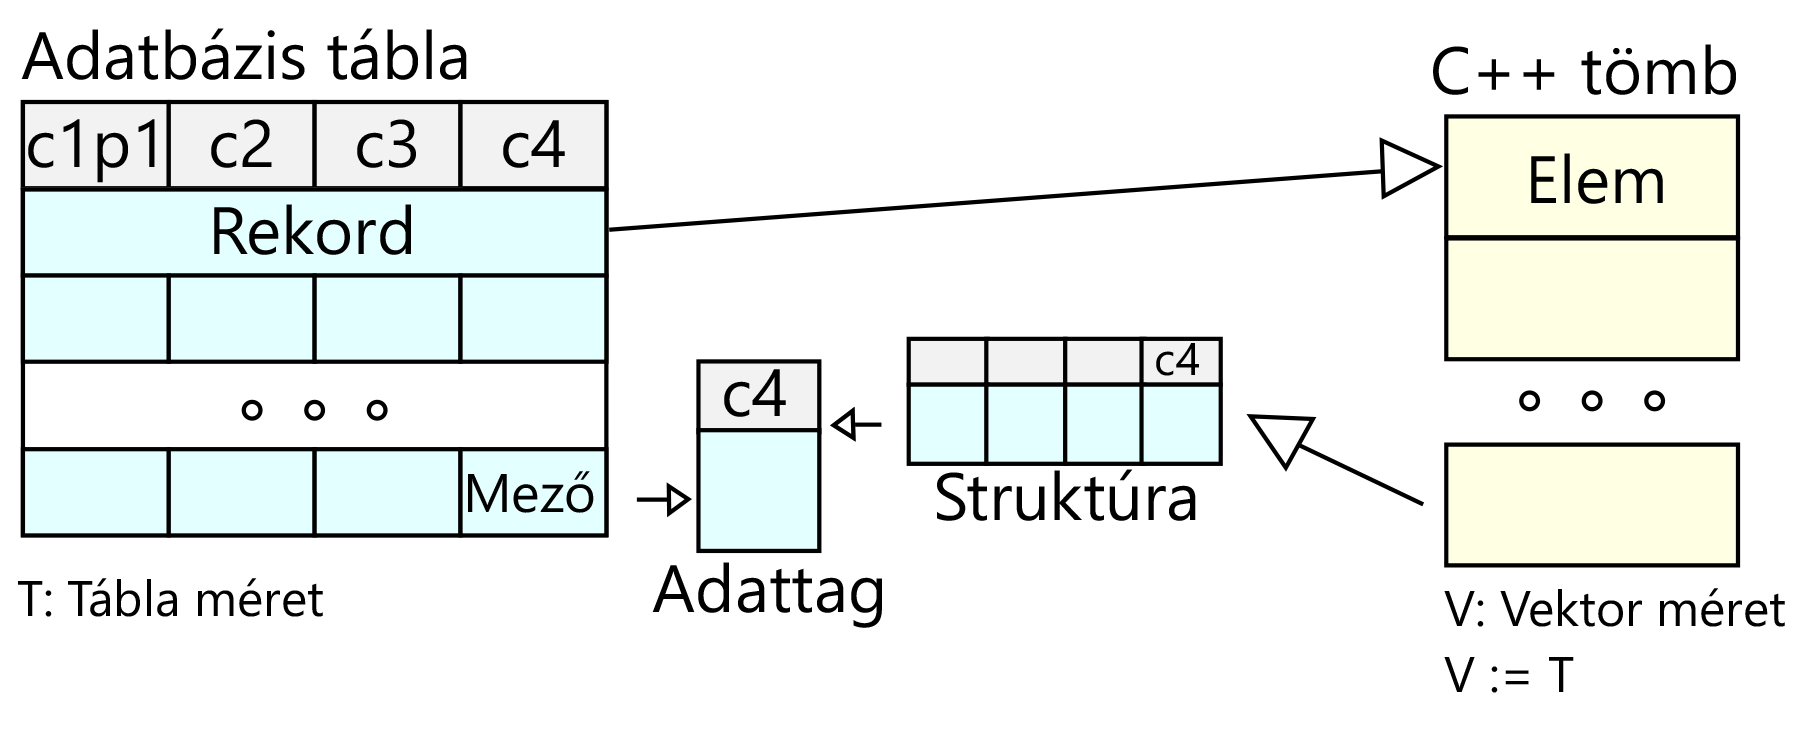
\includegraphics[width=11cm]{images/data/structure.png}
\caption{Adatbázistábla átalakítása tömbbé}
\label{fig:opencl}
\end{figure}

\begin{itemize}
\item A struktúra megfelel a tábla felépítésének.
\item A tömb egy eleme, egy ilyen struktúra.
\item A tömb egy eleme megfelel a tábla egy rekordjának azaz sorának.
\item Egy elem adattagjai megfelelnek az adatbázis egyazon rekordjához tartozó mezőknek.
\end{itemize}

\newpage
\SubSection{A táblákat beolvasó függvény.}

A fix sorszámmal rendelkező adatbázis táblák kezelése egy nagyon speciális eset lenne, ezért a programot úgy kell megírni, hogy igazodni tudjon a különböző táblaméretekhez.

Mivel a tábla méret előre nem ismert ezért a tömböket a \texttt{malloc} függvénnyel lehet lefoglalni. De mivel a lekérdezést külön függvény végzi, és a méretet sem tudjuk előre, ezért a következő megoldást alkalmazom:
Első lépésben létrehozok egy pointert ami később a táblára fog mutatni, most még \texttt{NULL} értékű, és ehhez egy változót ami a méretet tárolja. Az adatokat lekérő függvénynek átadom ezeket, és miután a \texttt{Connector} elvégezte a lekérdezést beállítom a méret változó értékét illetve a tábla memória területét csak ekkor foglalom le, és állítom rá a pointert. Ez úgy lehetséges, hogy a függvénynek egy pointerre mutató pointert adok át, ezáltal kettős indirektség jön létre.

\begin{cpp}
Table1Type *t1 = NULL;
int t1_size;
load_database(&t1, &t1_size);
	
res = pstmt->executeQuery();
\end{cpp}
\begin{figure}[h!]
\centering
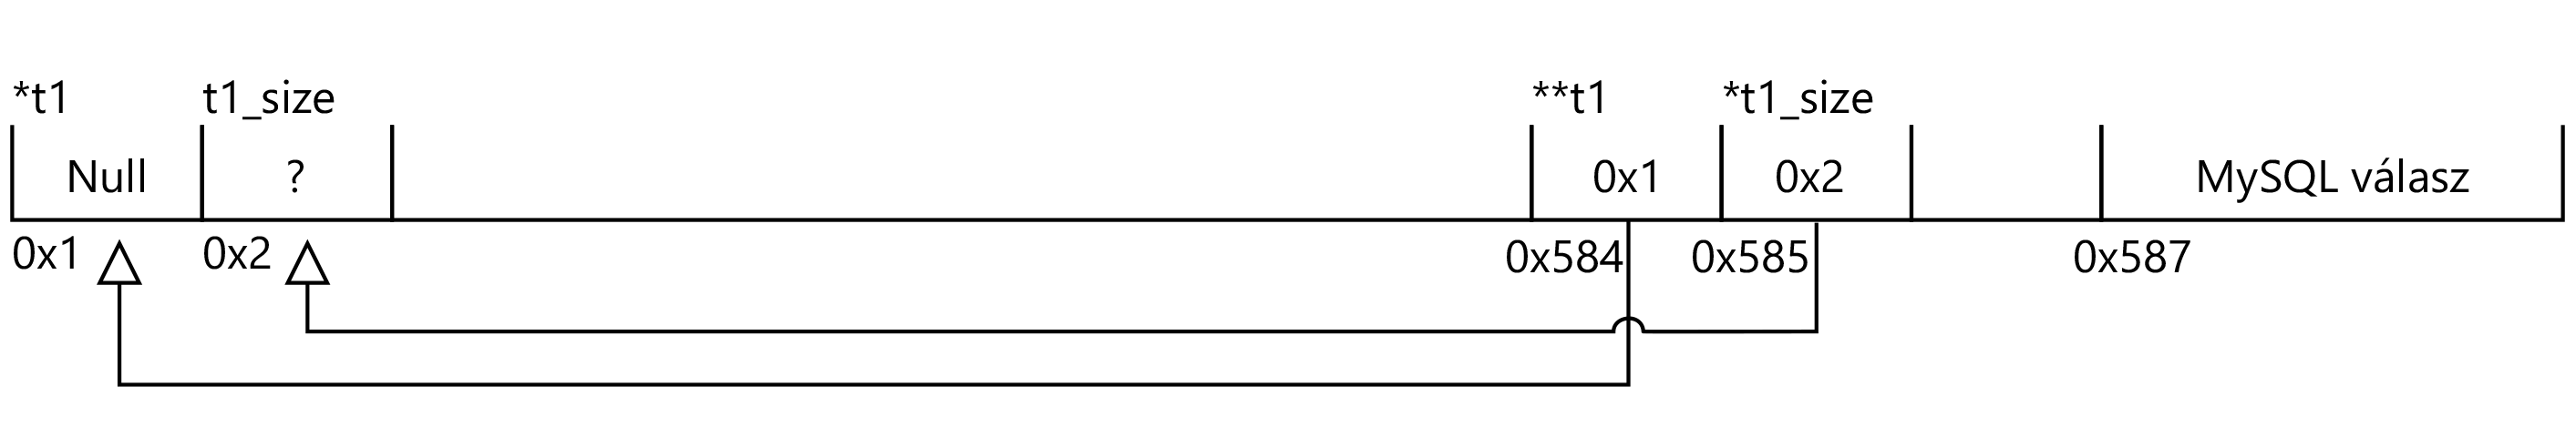
\includegraphics[width=\textwidth]{images/implementation/pointer_01.png}
\caption{Pointerek a létrehozáskor}
\label{fig:opencl}
\end{figure}
\begin{cpp}
int i = 0;
*T1_size = res->rowsCount();
*T1 = (Table1Type*) malloc(sizeof(Table1Type) * *T1_size);

while (res->next()) {
  T1[0][i].c1p1 = res->getInt("c1p1"); T1[0][i].c2 = res->getInt("c2");
  T1[0][i].c3 = res->getInt("c3"); T1[0][i].c4 = res->getInt("c4");
  i++;
}
\end{cpp}
\begin{figure}[h!]
\centering
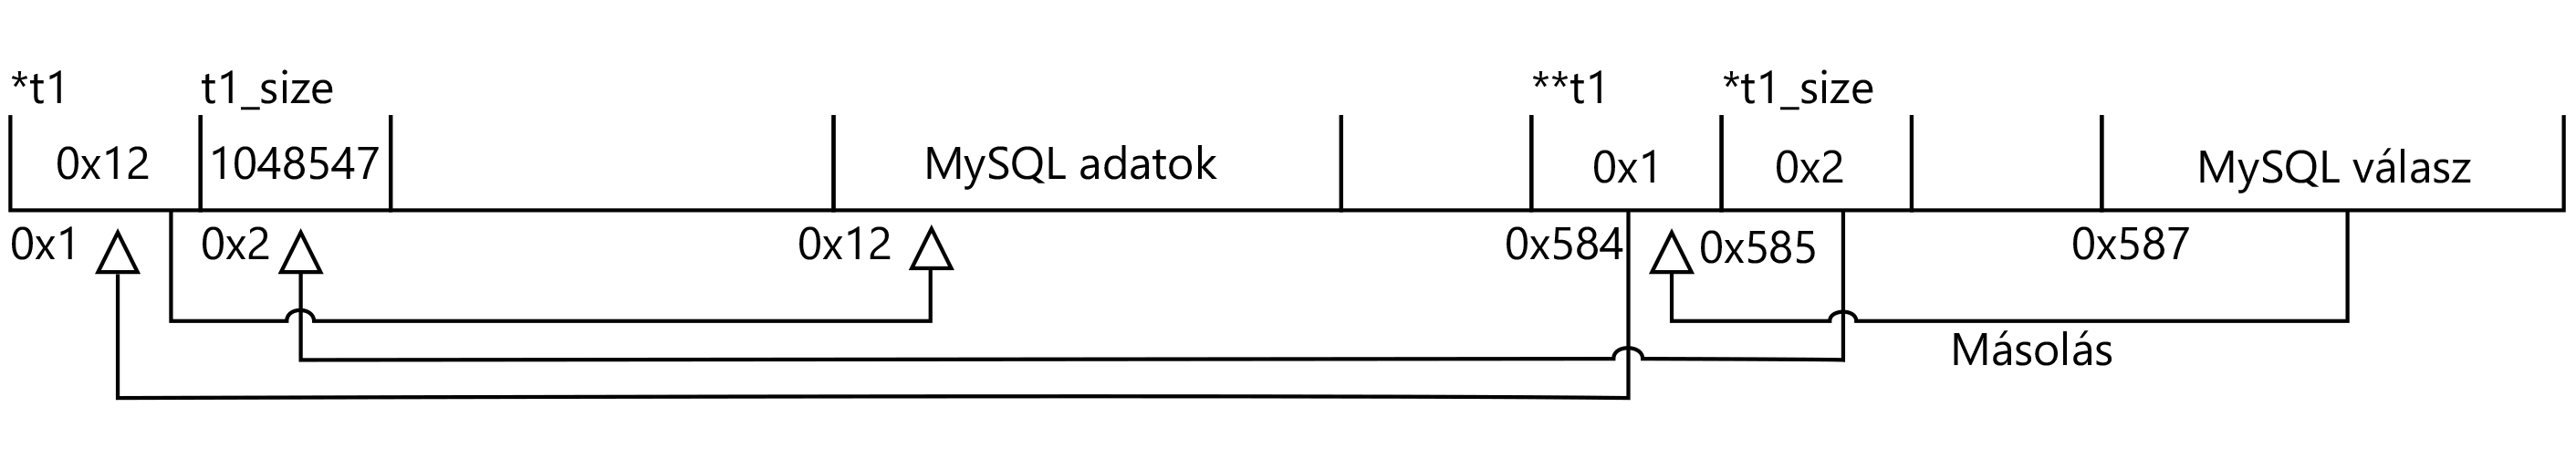
\includegraphics[width=\textwidth]{images/implementation/pointer_02.png}
\caption{Pointerek teljes működése}
\label{fig:opencl}
\end{figure}

\Section{Globális és lokális méret meghatározása}
Ennél a pontnál oda kell figyelni pár alapvető dologra:
\begin{itemize}
\item A lokális méret legfeljebb 1024 lehet.
\item A globális méretnek a lokális többszörösének kell lennie.
\item A túl sok vagy túl kevés munkacsoport használata esetén a párhuzamosság sérül.
\item A munkacsoportok és csoporton belül a munkaelemek feldolgozása párhuzamos.
\item Munkacsoportok között nem lehetséges szinkronizáció, csak munka elemek között, amennyiben azok egy munkacsoportba tartoznak.
\item Nem használható kölcsönös kizárás, a szemafor végtelen ciklushoz vezet.
\end{itemize}

\SubSection{Működési elv}

Egyszerű esetben a bementi elemszámot megadhatjuk mint globális méret, ez a gyakorlatban meghatározza, hogy hányszor fog lefutni a kernel függvény. A $get\_global\_id(0)$ meghívásával megkapjuk az aktuális azonosítót, ez 0 -tól globális méret -1 ig terjed. Innentől tekinthetünk a teljes kódra úgy, mintha egy párhuzamos futó \texttt{for} ciklusban lenne.

Ezen kívül meg kell adnunk a lokális méretet, ami az elemek száma egy munkacsoporton belül. A kernel futása közben ezt is megkaphatjuk a $get\_local\_id(0)$ használatával, csak úgy mint a munkacsoport azonosítót vagy az említett paraméterek méretét.

A végeredményt tartalmazó kimeneti tömb hossza egyezik a globális mérettel, így nem ütközhetünk bele abba a hibába, hogy két számítási elem ugyan oda próbáljon írni. Amennyiben például az 545. elem megfelel, akkor az indexe és egyéb hozzá tartozó értékek az 545. helyen lesznek a kimeneti tömbben.

\begin{figure}[h!]
\centering
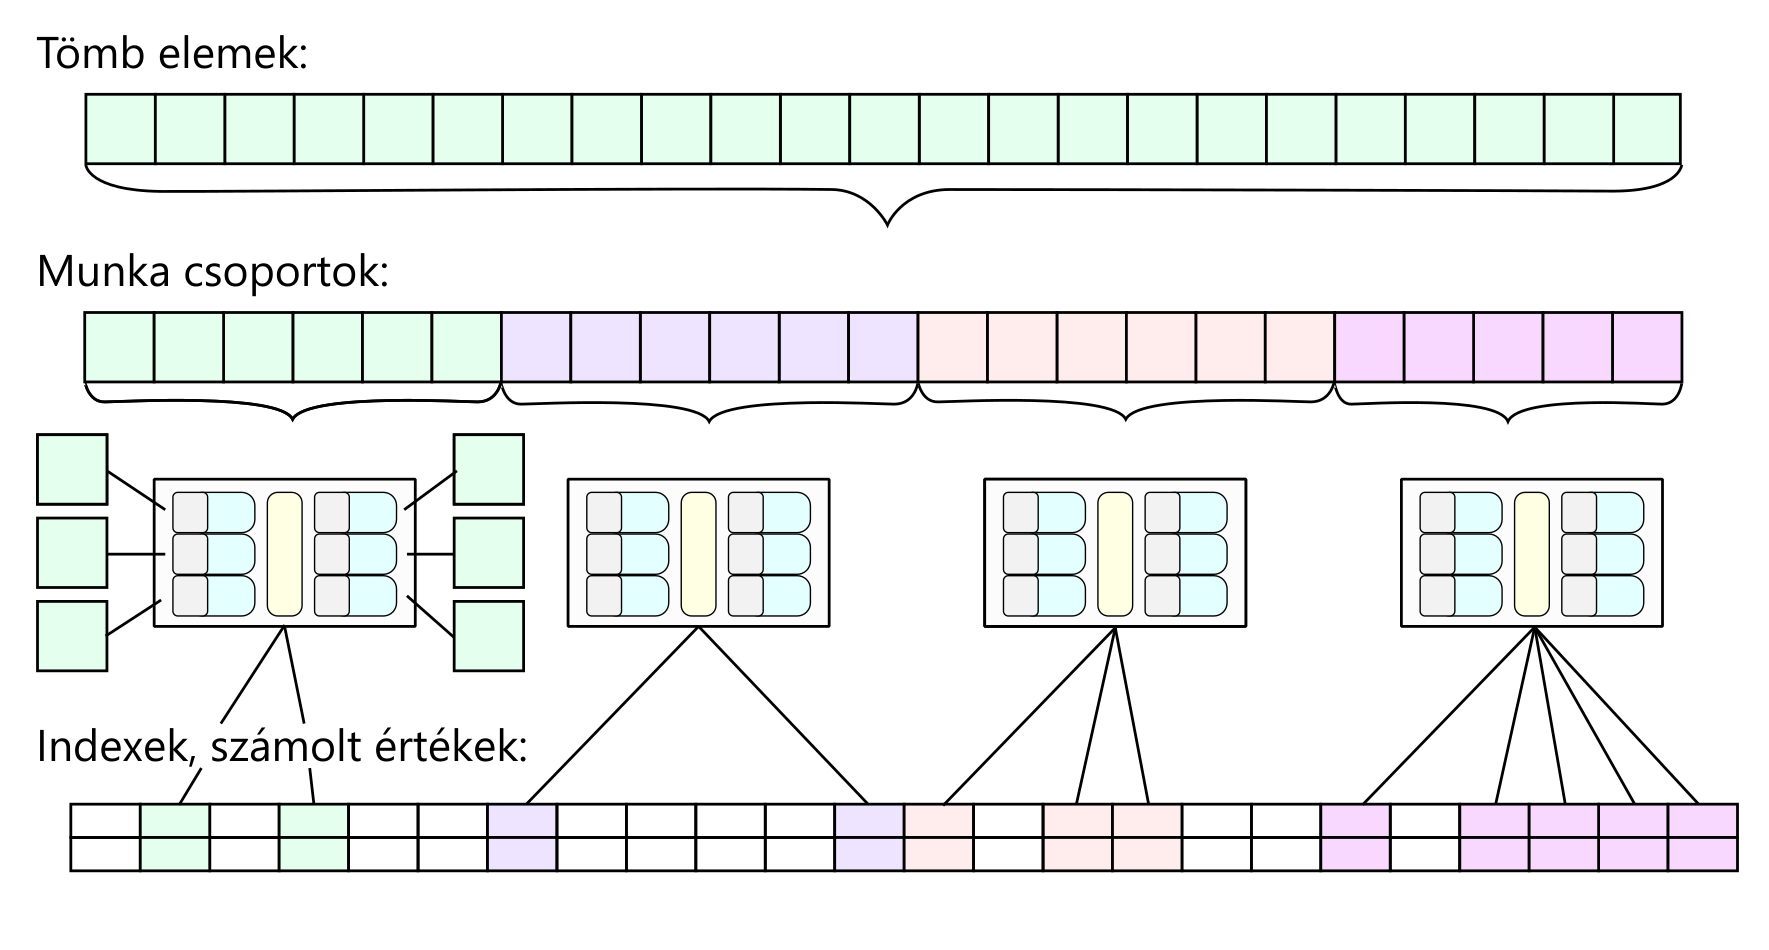
\includegraphics[width=\textwidth]{images/workgroups_black.png}
\caption{Munkacsoportokra bontás}
\label{fig:opencl}
\end{figure}

\newpage

\SubSection{Globális méret meghatározása}
Tegyünk fel, hogy kaptunk egy 1048547 sorból álló táblázatot. Ekkor több probléma is előkerül. Egyrészt olyan lokális méretet kell választani ami ennek a számnak az osztója. Másfelől nem szeretnénk végignézni az ugyan ilyen hosszú kimeneti tömböt az eredmények helyét keresve.

A következő módon oldottam meg a problémát: Állítsuk a globális méretet például 1024 -re, ehhez határozzunk meg egy intervallum méretet a sorok száma és globális méret hányadosának felső egész része ként. Ez jelen esetben szintén 1024 lesz. Viszont így át kell adnunk a kernelnek a tábla méretét, ami felső határként ügyel arra, hogy ne lépjük túl a tömböt méretét.

A módosításnak az lesz a következménye, hogy egy munkaelem nem csak a tömb egy elemén fog dolgozni hanem egy intervallumán. Ezzel létrehoztunk olyan részeket a tömbben amiknek a feldolgozása biztosan soros lesz. Ennek köszönhetően már tudunk használni számlálókat, nincs szükség kölcsönös kizárásra. A számlálókat tartalmazó tömb mérete megegyezik a globális mérettel.

Ezekhez a paraméterekhez még tetszőlegesen meg kell határozni a lokális méretet, aminek csak a teljesítményre van hatása.


$$ global\_size = 1024 $$
$$interval\_size =  \left\lfloor \frac{table\_size }{globalsize\_size} \right\rfloor  +1  $$


\SubSection{A kernelkód működése}

A kernel meghatározza saját globális azonosítóját és ebből illetve a kapott intervallum méretből kiszámítja, honnan kezdőik az ő része a be-, és kimeneti tömbön. Ezután elkezdi az intervallumnyi elem vizsgálatát ügyelve arra, hogy a tábla méretet ne lépje túl. Amennyiben egy elem megfelel a szűrési paramétereknek annak indexét és egyéb lekérdezés függő kiszámolt értékeket a kimeneti tömbbe másol, majd növeli saját számlálóját. Ez a számláló határozza meg, hogy a kimeneti szakaszon a következő elem hányadik helyre kerüljön.
\begin{figure}[h!]
\centering
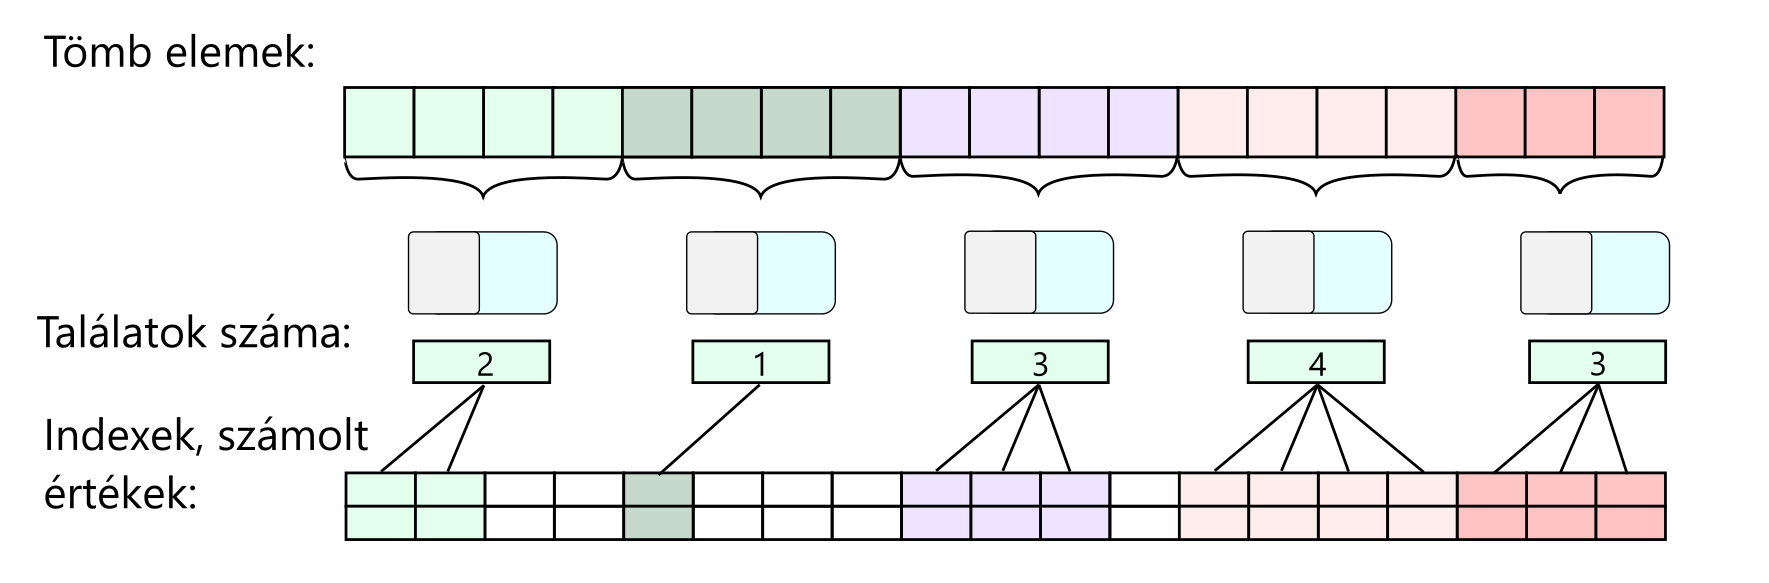
\includegraphics[width=\textwidth]{images/itemgroup_black.png}
\caption{Intervallumok feldolgozása}
\label{fig:opencl}
\end{figure}
Itt már nem munkacsoportonként, hanem feldolgozó elemenként látjuk a folyamatot.

\newpage
\Section{Eredmény kiolvasása}
A kernelkód működéséből látjuk, hogy több módszert is tudunk alkalmazni az elemek kiolvasására. A találatok számát tartalmazó tömböt biztosan ki kell másolnunk, de kimenetre vonatkozóan nézzük meg az alábbi lehetőségeket.
\SubSection{Az elemek kiolvasása egyben}

Dönthetünk úgy, hogy kimásoljuk a teljes kimenetet:
\begin{python}
clStatus = clEnqueueReadBuffer(command_queue, TableResult_clmem, 
	CL_TRUE, 0, table_size * sizeof(TableResultType), result, 
	0, NULL, NULL);
\end{python}
Ekkor ennek olvasása a következőképpen zajlik:
\begin{python}
for(i=0; i< global_size; i++)
{
  offset = i*interval_size;
  
  for(j=0; j<result_counter[i]; j++)
  	cout << t1[ result[ offset + j ].index ].c1p1 << endl;
}
\end{python}
Végig kell menni a számlálón aminek hossza \texttt{global size}, majd az \texttt{ i * interval size} eltolást használva annyi elemet kell sorban kiolvasni az adott részről, amekkora érték a hozzá tartozó számlálóban található. Ezzel végig lépkedve és ugrálva a kimeneten ki tudjuk olvasni az indexeket illetve kiszámított értékeket.

\SubSection{Az elemek kiolvasása szakaszosan}
A másik módszer, hogy csak az információkat tartalmazó részeket olvassuk a pufferekből. Ez hasonló módon zajlik, mint előző esetben az eredmények kiírása.

\begin{python}
int count = 0;
for(int i=0; i< global_size; i++)
{
if(result_counter[i] < 1 ) continue; 
clStatus = clEnqueueReadBuffer(command_queue, TableResult_clmem, CL_TRUE, 
	i*interval_size * sizeof(TableResultType),
	result_counter[i]* sizeof(TableResultType), 
	&result[count], 0, NULL, NULL);
	count+=result_counter[i];
}
\end{python}

Kiolvasásnál megadjuk az eltolást amit az előző módon számolunk annyi különbséggel, hogy megadjuk egy elem memória méretét:
$$i * interval\_size * sizeof(TableResultType)$$ezután megadjuk, hogy az eltolástól kezdve mekkora memória méretet szeretnénk kiolvasni: $$result\_counter[i] * sizeof(TableResultType)$$Ezen kívül a másolás cél memóriacímét mindig eltoljuk, az eddigi találatok számával: $$\&result[count].$$
Ha memóriát is szeretnénk spórolni, megtehetjük azt is, hogy először összeadjuk a találatokat és az alapján foglaljuk le a memóriaterületet a kiolvasáshoz.
\begin{figure}[h!]
\centering
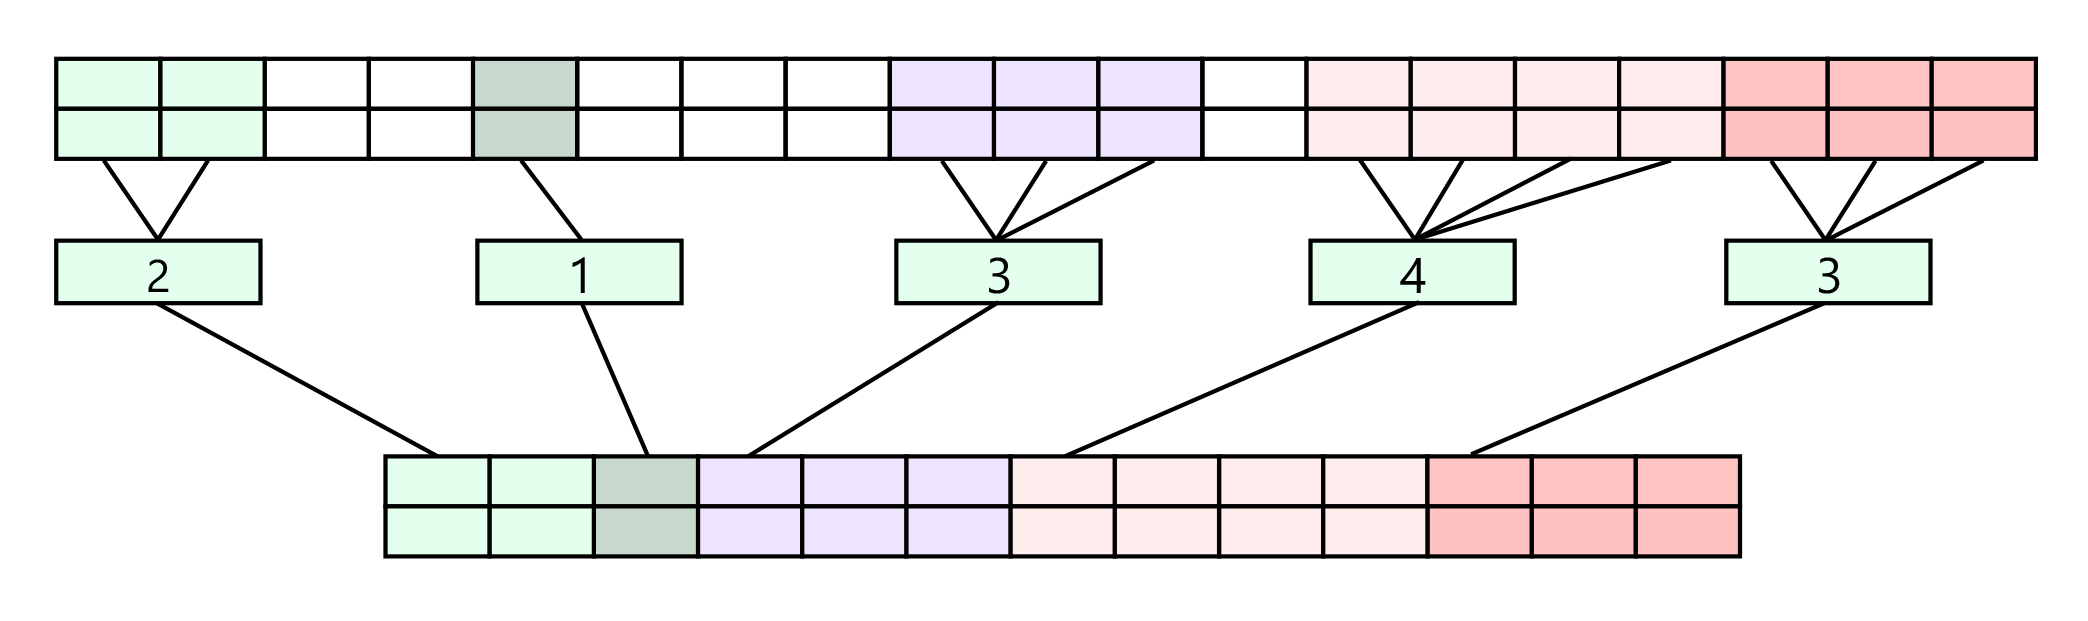
\includegraphics[width=\textwidth]{images/copy_02.png}
\caption{Szelektív eredménykiolvasás}
\label{fig:opencl}
\end{figure}
\newpage
\Section{Összetett lekérdezés}

Az előzőekben taglalt elméleti részek egy táblás lekérdezésekre vonatkozóan próbálták szemléltetni, milyen logika alapján lehet egy \texttt{SQL} lekérdezést \texttt{GPU} -n párhuzamosítva végrehajtani.
Most gondoljuk át, miképpen lehetne megoldani kettő vagy több tábla összekapcsolását. Első lépésben a lekérdezést egy-egy táblára vonatkozó részekre. Ezzel két tábla kapcsolása esetén létrejöhet két különálló kernel amelyek például a szűréseket végzik a táblákon. Ennél a lépélnél két dolgot is szükséges kiemelni. Egyrészt ezeknek a kerneleknek az előállított eredményét nem kell kiolvasni a pufferekből, ugyanis ez a globális memóriában van, így átadható másik kernel számára is. Másrészt pedig ezek a kernelek ha van kapacitás, akkor futhatnak párhuzamosan is, ezt úgy lehet elérni, hogy külön parancssort hozunk létre számukra.

Miután minden nem összekapcsolást végző kernel befejezte a munkát, adjuk át a szükséges paramétereket a befejező kernelnek. A paraméter lista elég hosszú lesz, ennek az az oka, hogy az eredmények kiolvasása elő észében taglalt módon kell végig menni a szűrt táblákon. 

Ennek a kernelnek a globális mérete egyezzen meg a lekérdezésben szereplő legnagyobb tábla globális méretével és ez a tábla szerepeljen a külső ciklusban. Az eredményeket változatlan módokon lehet majd kiolvasni a főprogramba.

\begin{figure}[h!]
\centering
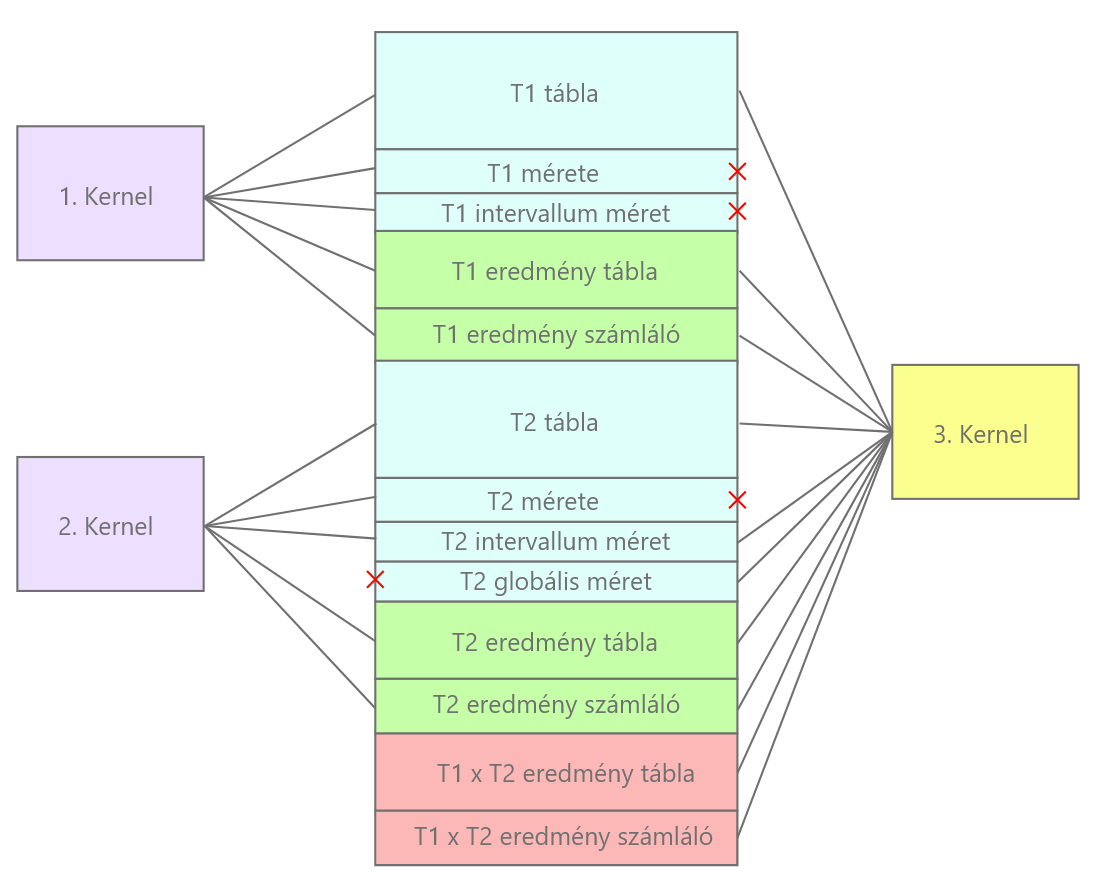
\includegraphics[width=12cm]{images/join_kernels.png}
\caption{Kernelek munkaterületei }
\label{fig:opencl}
\end{figure}

Az 1. és 2. kernel az előzőekben taglalt módon előállítja saját eredményeit (zöld rész). 
A 3. kernel megkapja a két táblát, a 2. tábla méretét és az előző két kernel által előállított eredményeket.
Az első eredmény kiolvasási módszer alkalmazásával és a kulcsok figyelésével a két táblát összekapcsoljuk és előállítjuk az eredményt.
A táblák méretére nincsen szükség, ugyanis az eredmény biztosan nem tartalmaz olyan indexet ami kívül esne az eredeti táblákon. A második táblánál viszont szükség van a globális méretre és az intervallum méretre a kiolvasáshoz.

\Chapter{Mérések, összehasonlítások}

%Ebben a fejezetben megvizsgáljuk a program különböző részeit futási idő szempontjából. Első sorban nézzük azokat a részeket amelyek nagyban függnek a táblamérettől vagy az előállítani kívánt kimenettől.  

\Section{Adatok mozgatásának sebességei}

Ebben a részben azt vizsgálom, hogy mennyi idő eljuttatni az adatokat a \texttt{MySQL} szerverről a memóriába, azokat pufferekbe másolni, majd onnan az eredményeket visszaolvasni.
Annak érdekében, hogy a mérések pontosabbak legyenek, minden eredmény 5 futás átlagából került kiszámításra.

\SubSection{A \texttt{MySQL} lekérdezés sebessége}

A méréseket a programok között, a \texttt{sql\_speed} nevű mappában található kódokkal végeztem.

Ezt a sebességet a következő két sor vizsgálatával kaphatjuk meg a legpontosabban:
\begin{python}
pstmt = con->prepareStatement(command);
res = pstmt->executeQuery();
\end{python}
A  \texttt{res} és \texttt{pstmt} törlése időméréskor nagyon fontos, ugyanis ennek kihagyása miatt a memória megtelhet!
A \texttt{command} egy \texttt{string} az \texttt{SQL} parancs és a következő módon áll össze:
\begin{python}
range = 32768;
while (i <= 1048576)
{
   command = "SELECT * FROM speedtest_1048576 Limit " + to_string(i);
   // ...
   i += range;
}
\end{python}
\begin{itemize}
\item A LIMIT hozzáadása a lekérdezéshez nem növeli annak idejét.
\item A tábla tartalmaz elsődleges kulcsot, enélkül a lekérdezések ideje megnő.
\item A lekérdendő oszlopokat manuálisan módosítottam a programban: 
\begin{itemize} 
\item \texttt{SELECT c1p1 FROM ...}
\item \texttt{SELECT c1p1, c2 FROM ...} 
\item \texttt{SELECT c1p1, c2, c3 FROM ...} 
\item \texttt{SELECT * FROM ...} 
\end{itemize}
\end{itemize}

\begin{figure}[h!]
\centering
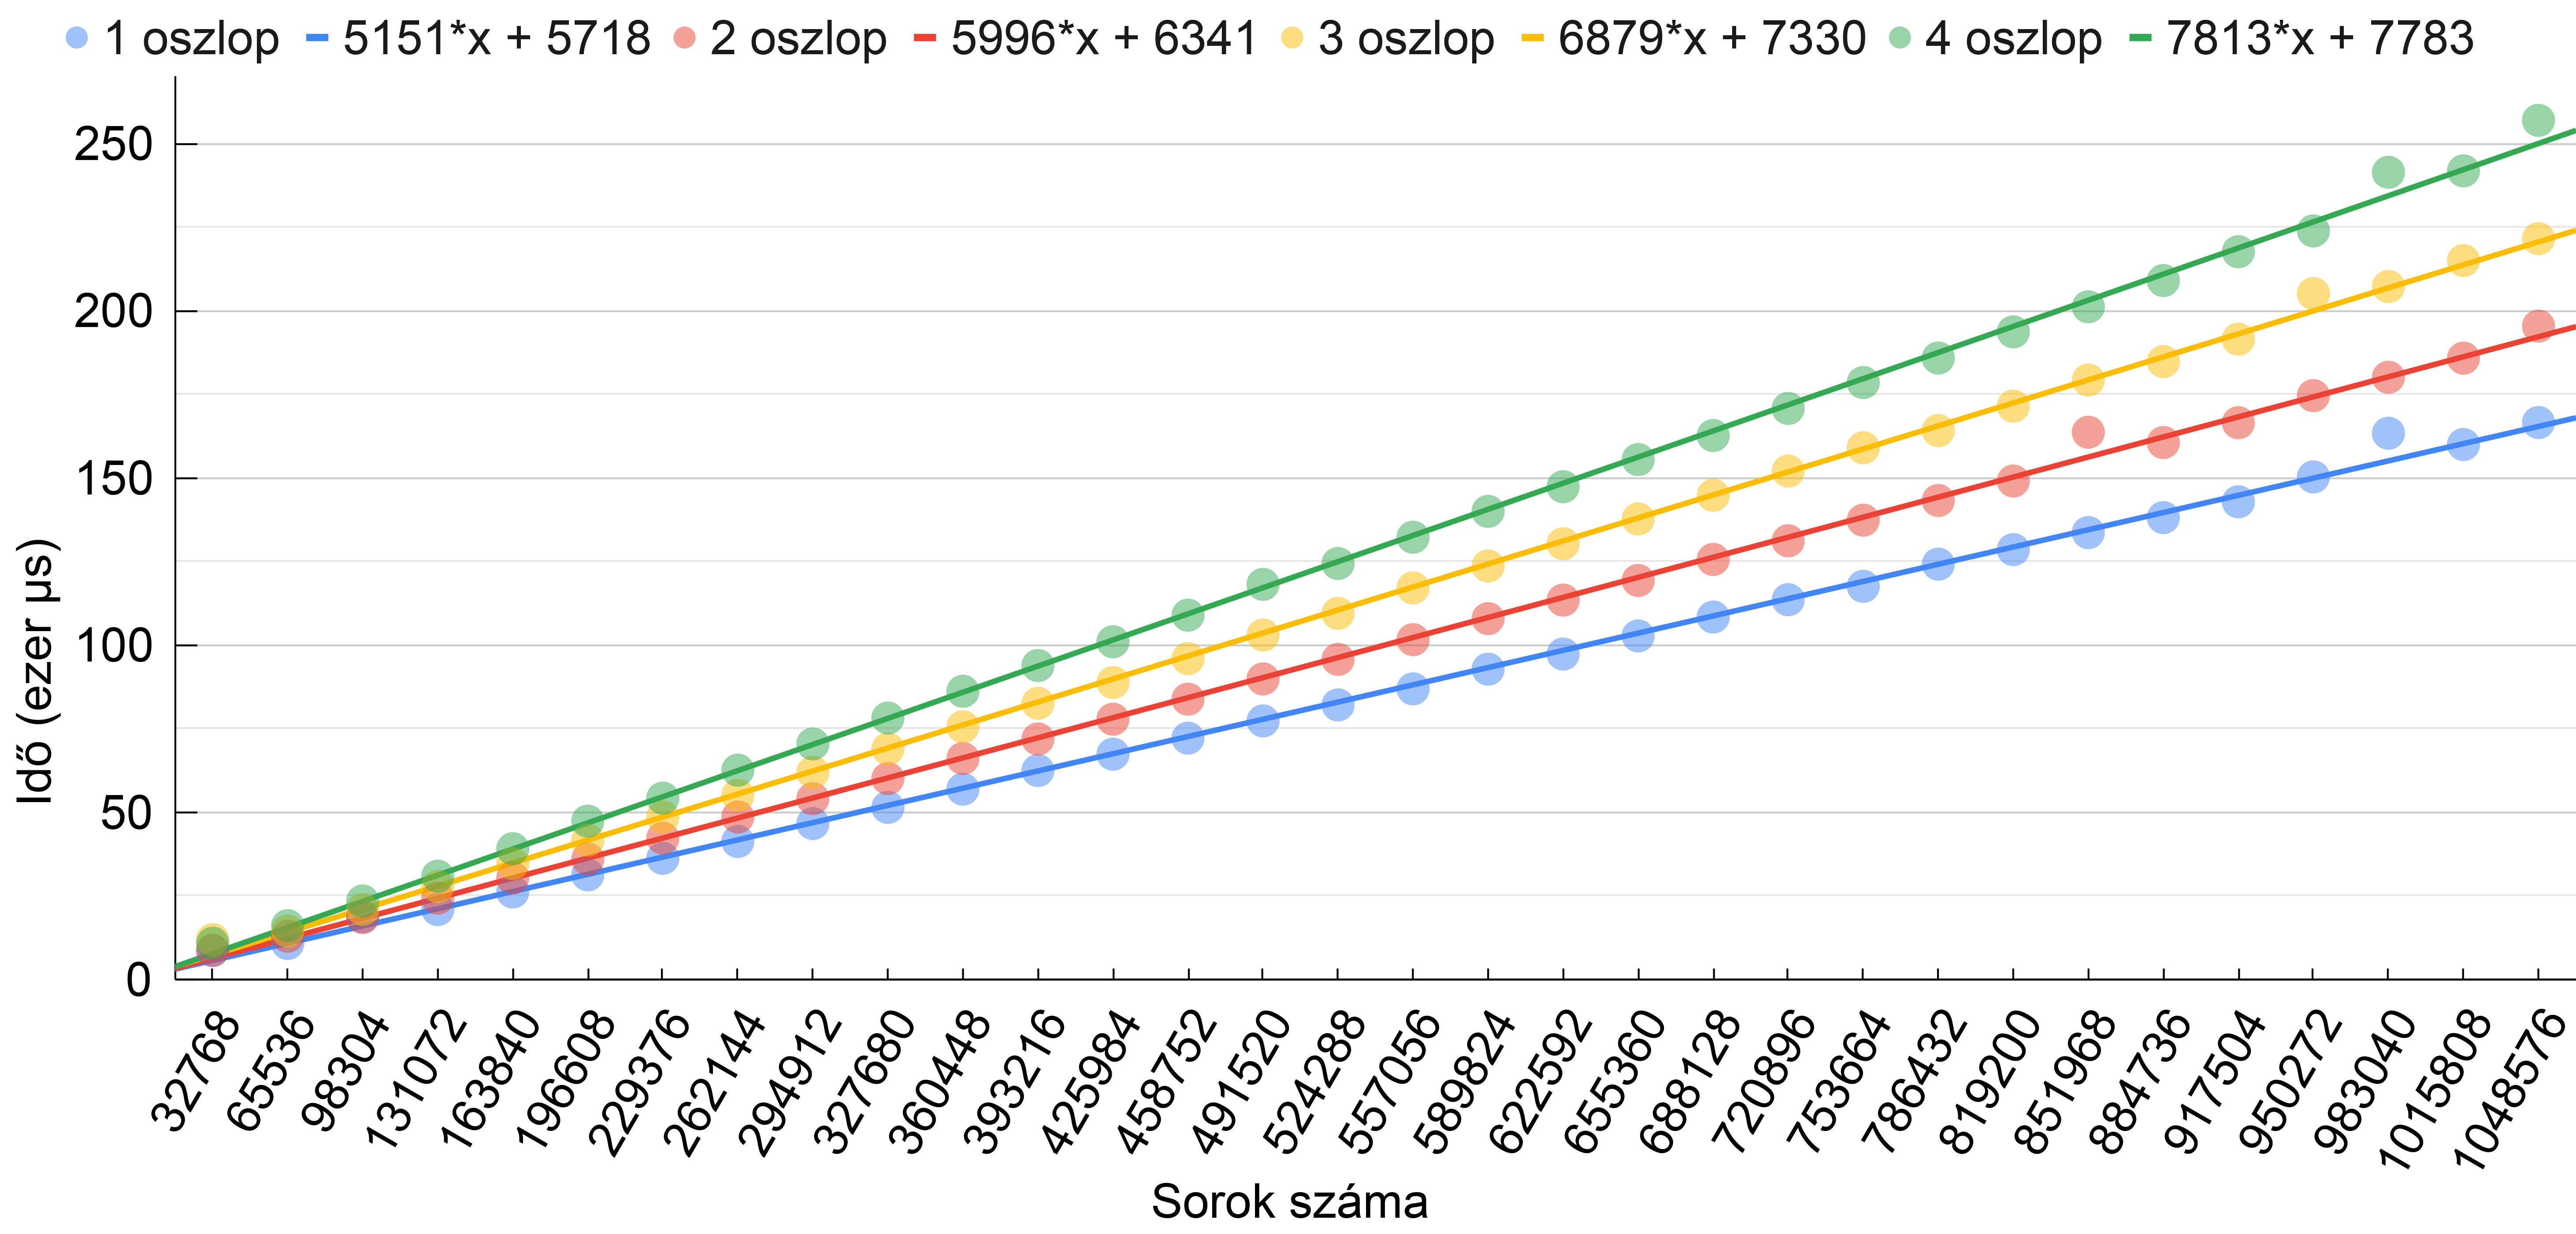
\includegraphics[width=\textwidth]{images/graph/sqlquery.png}
\caption{Az SQL lekérdezési sebessége}
\label{fig:sqlquery}
\end{figure}

\Aref{fig:sqlquery}. ábrán, egyértelműen látható, hogy a sorok számának növekedésével az idő is lineárisan nő.
A jelmagyarázatnál látható egyenes egyenletekből becsléseket lehet készíteni adott paraméterekkel rendelkező szűrés nélküli lekérdezéshez. 

Négy oszlop felett használjuk a 3 és 4 oszlop közötti növekedés mértékét, feltételezve, hogy innentől ez már nem változik. A kettő között eltérés lineáris becslésének képlete: 
$$7,79 \cdot 10^{-5} \cdot x + 1,13, \quad R^2=0,992,$$ 
ahol
$$x = \dfrac{\text{sorok száma}}{32768} - 1.$$
4 oszlop esetén:
$$ 7813 \cdot \text{sorok száma} + 7783 = \text{lekérdezés ideje}.$$

\SubSection{A query válaszának átmásolása a saját tömbbe}

A vizsgálathoz használt kód a programok \texttt{cp\_to\_array} nevű mappájában található.

A lekérdezésből kapott választ át kell másolni az általunk létrehozott tömbbe. Ez az egyik legköltségesebb művelet, ezért optimalizálásként itt is célszerű csak a felhasznált oszlopokat lekérni.
A mért program szakasz:
\begin{python}
int i = 0;
*T1_size = res->rowsCount();
*T1 = (Table1Type*) malloc(sizeof(Table1Type) * *T1_size);

while (res->next())
{
    T1[0][i].c1p1 = res->getInt("c1p1");
    // ...
    T1[0][i].c4 = res->getInt("c4");
    i++;
}
delete res;
delete pstmt;
\end{python}
Itt a válaszból lekérdezzük a méretet, majd ez alapján létrehozzuk a saját objektumunkat a memóriában, ezután egyesével belemásoljuk a kapott adatokat soronként.
Az mérési módszer megegyezik az előzőekben használtakkal.

\begin{figure}[h!]
\centering
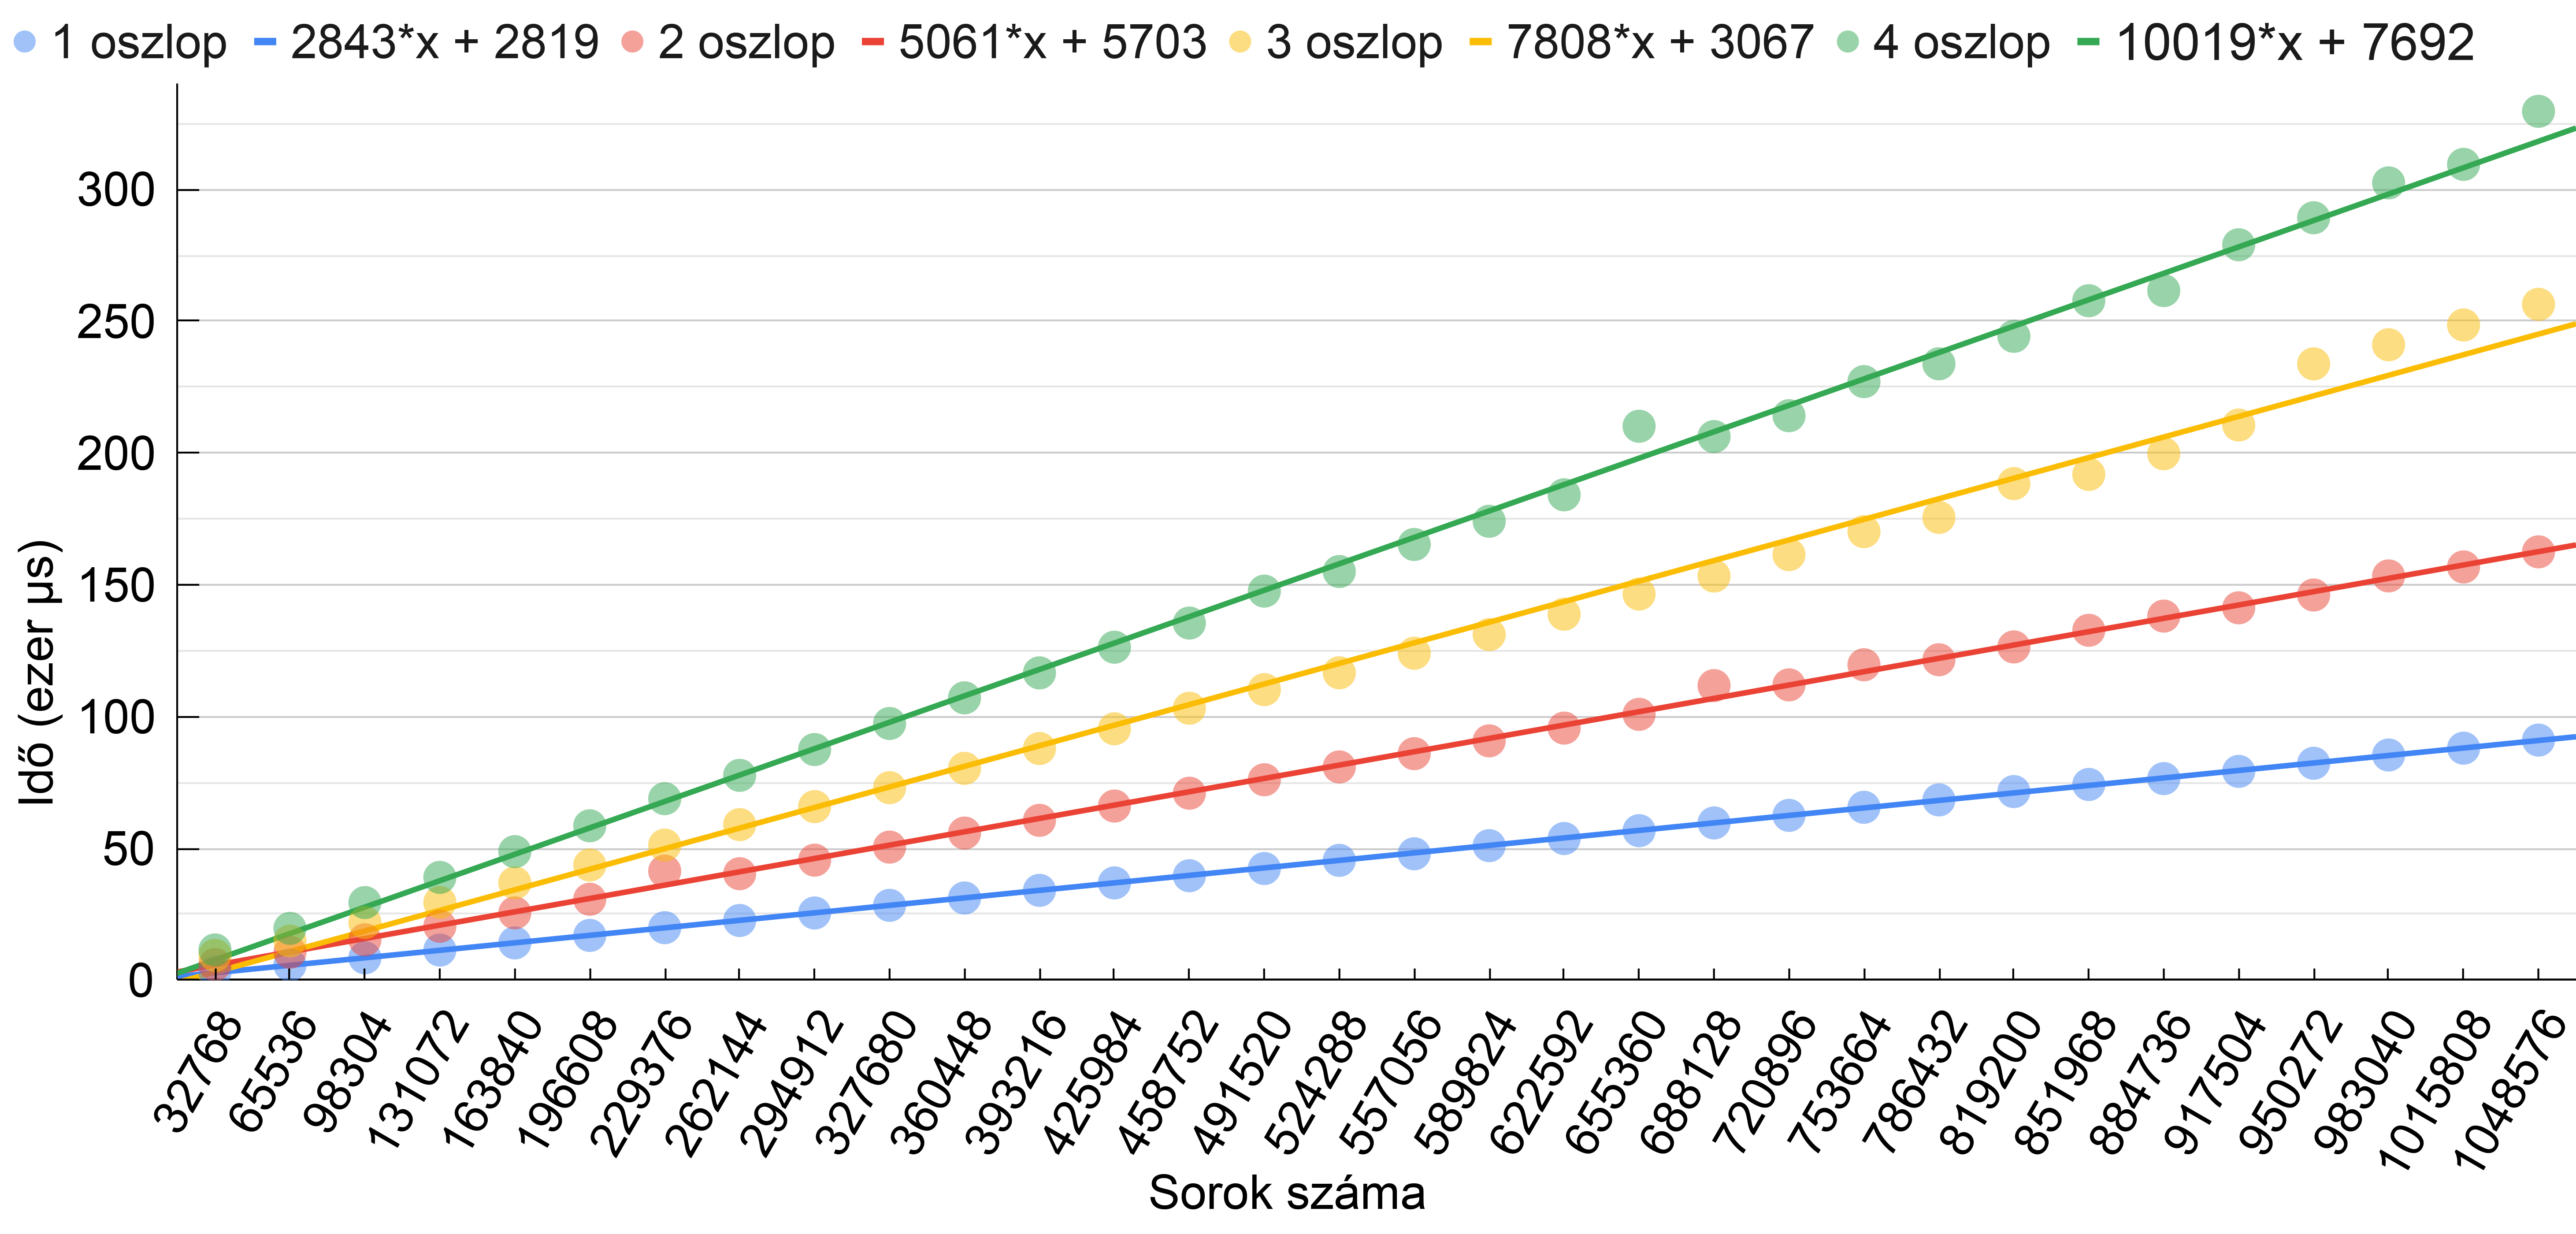
\includegraphics[width=\textwidth]{images/graph/ccopy.png}
\caption{Adatok másolása saját tömbbe}
\label{fig:ccopy}
\end{figure}

\Aref{fig:ccopy}. ábrán látható grafikonon két dolgot vehetünk észre azonnal. Az egyik az, hogy ez a folyamat lassabb, mint maga a lekérdezés. A másik pedig, hogy drasztikusabb a növekedés az oszlopok számának sokasodásával.
Tételezzük fel, csak úgy mint az előző esetben, hogy 4 oszlop felett nem több az elérés, mint 3 és 4 között.
A két oszlop közötti eltérés lineáris becslése:
$$-6,1 \cdot 10^{-4} \cdot x + 1,32, \quad R^2=0,99,$$ 
ahol
$$x = \dfrac{\text{sorok száma}}{32768} - 1.$$
Becslés 4 oszlop esetén:
$$ 10019 \cdot x + 7692 = \text{másolás ideje}$$

\SubSection{Adatok bemásolása a pufferekbe}

Az adatok átmásolása az \texttt{OpenCL} puffereibe szintén egy olyan része a programnak, ami sok időt emészthet fel.
(Az ehhez elkészített program neve \texttt{cp\_buffer}.)
Vizsgáljuk meg a következő kódrészt.
\begin{python}
int range = 65536;
while (range <= 1048576)
{
 clStatus = clEnqueueWriteBuffer(command_queue, Table1_clmem,
  CL_TRUE, 0, range * sizeof(Table1Type), t1, 0, NULL, NULL);
 clStatus = clEnqueueWriteBuffer(command_queue, Table_size_clmem,
  CL_TRUE, 0, sizeof(int), &t1_size, 0, NULL, NULL);
 clStatus = clEnqueueWriteBuffer(command_queue, Interval_size_clmem,
  CL_TRUE, 0, sizeof(int), &interval_size, 0, NULL, NULL);
 clStatus = clFinish(command_queue);
 range += 65536;
}
\end{python}

\begin{figure}[h!]
\centering
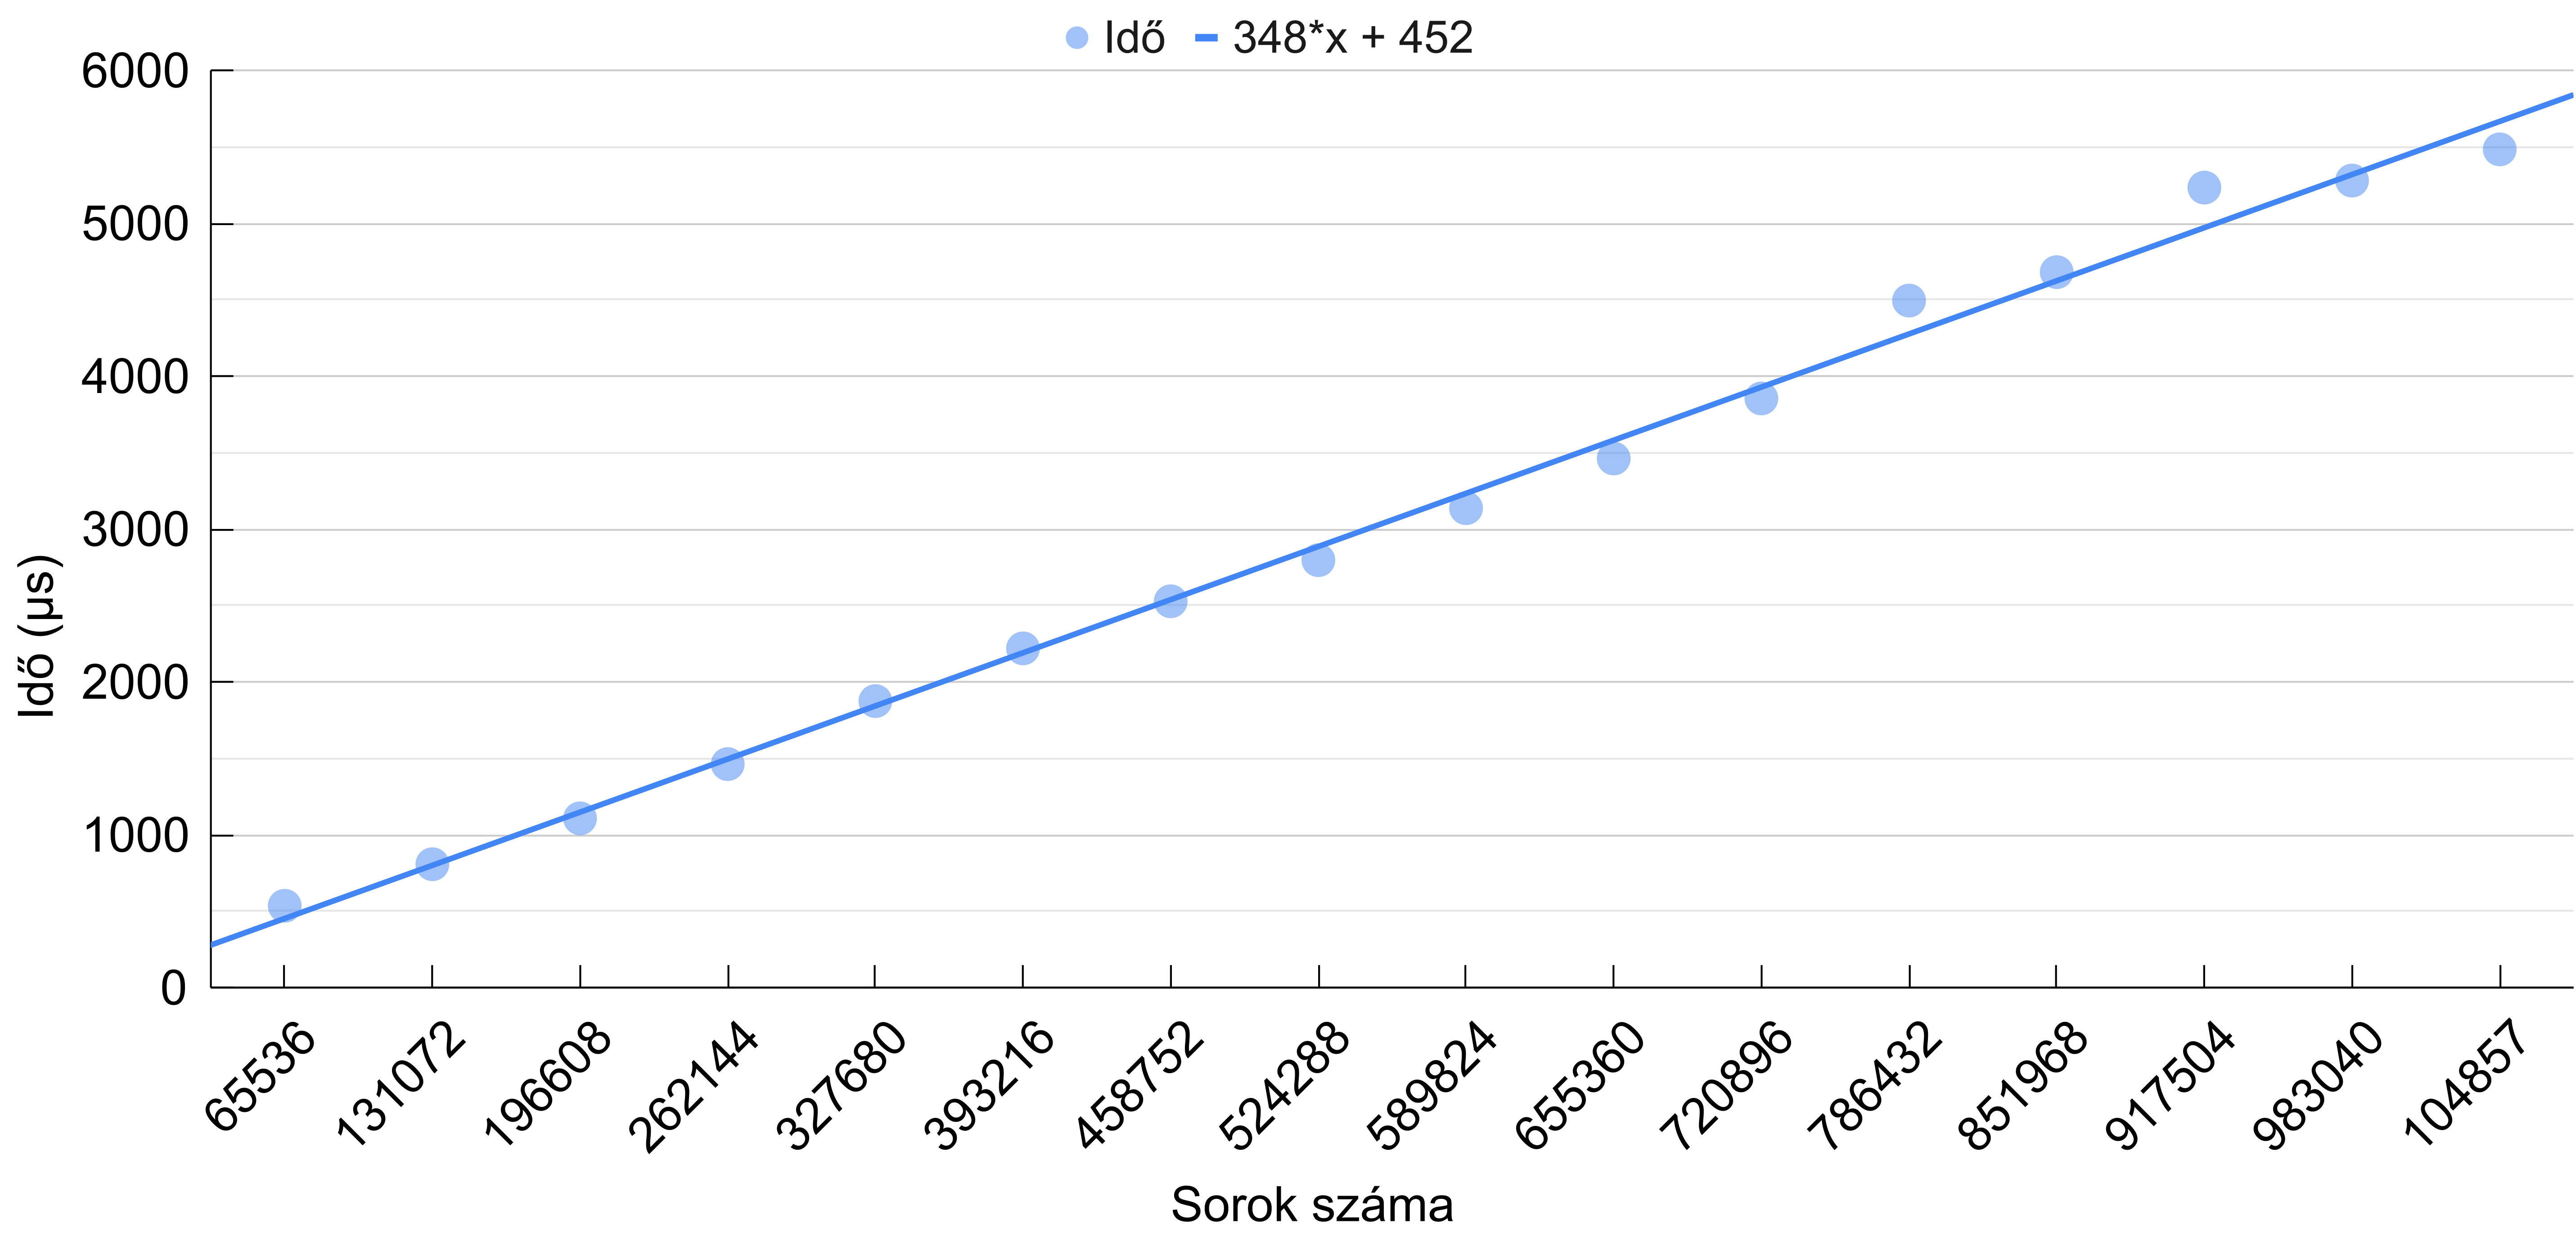
\includegraphics[width=\textwidth]{images/graph/pufferin.png}
\caption{Adatok bemásolása 2.}
\label{fig:pufferin}
\end{figure}

Mivel ebben az esetben a másolás egybefüggő memória területre vonatkozik, nem pedig elemenkénti hivatkozás, ezért elegendő egyetlen mérés.
\Aref{fig:pufferin}. grafikonon egy 4 oszlopos tábla átmásolásának a sebessége látható. Ebből több vagy kevesebb oszlopra, illetve sorra a becslés egyszerű szorzásokkal megkapható.

3 és 4 oszlop esetén:
$$ x = \text{sorok száma} / 65536, $$
$$ 348 \cdot x + 452 = \text{pufferbe másolás ideje}, $$ 
$$ \text{pufferbe másolás ideje} \cdot 0.75 = \text{3 oszlopos pufferbe másolás ideje}. $$

\SubSection{Adatok kimásolása a pufferekből}

Nézzük az első kiolvasási módszert, amikor a teljes eredmény tömböt illetve a hozzá tartozó számlálót másoljuk ki.
Jelen mérésnél a lista csak egyetlen indexet tartalmaz:
$$ x = \text{sorok száma} / 65536, $$
$$ 81,2 \cdot x + 156 = \text{puffer kiolvasási ideje}. $$ 
Az előzőhöz hasonlóan itt is egy memória darabot másolunk, ennek szorzásával megkapjuk mennyi időbe telne a kiolvasás más méretek esetén (\ref{fig:pufferout}. ábra).

\begin{figure}[h!]
	\centering
	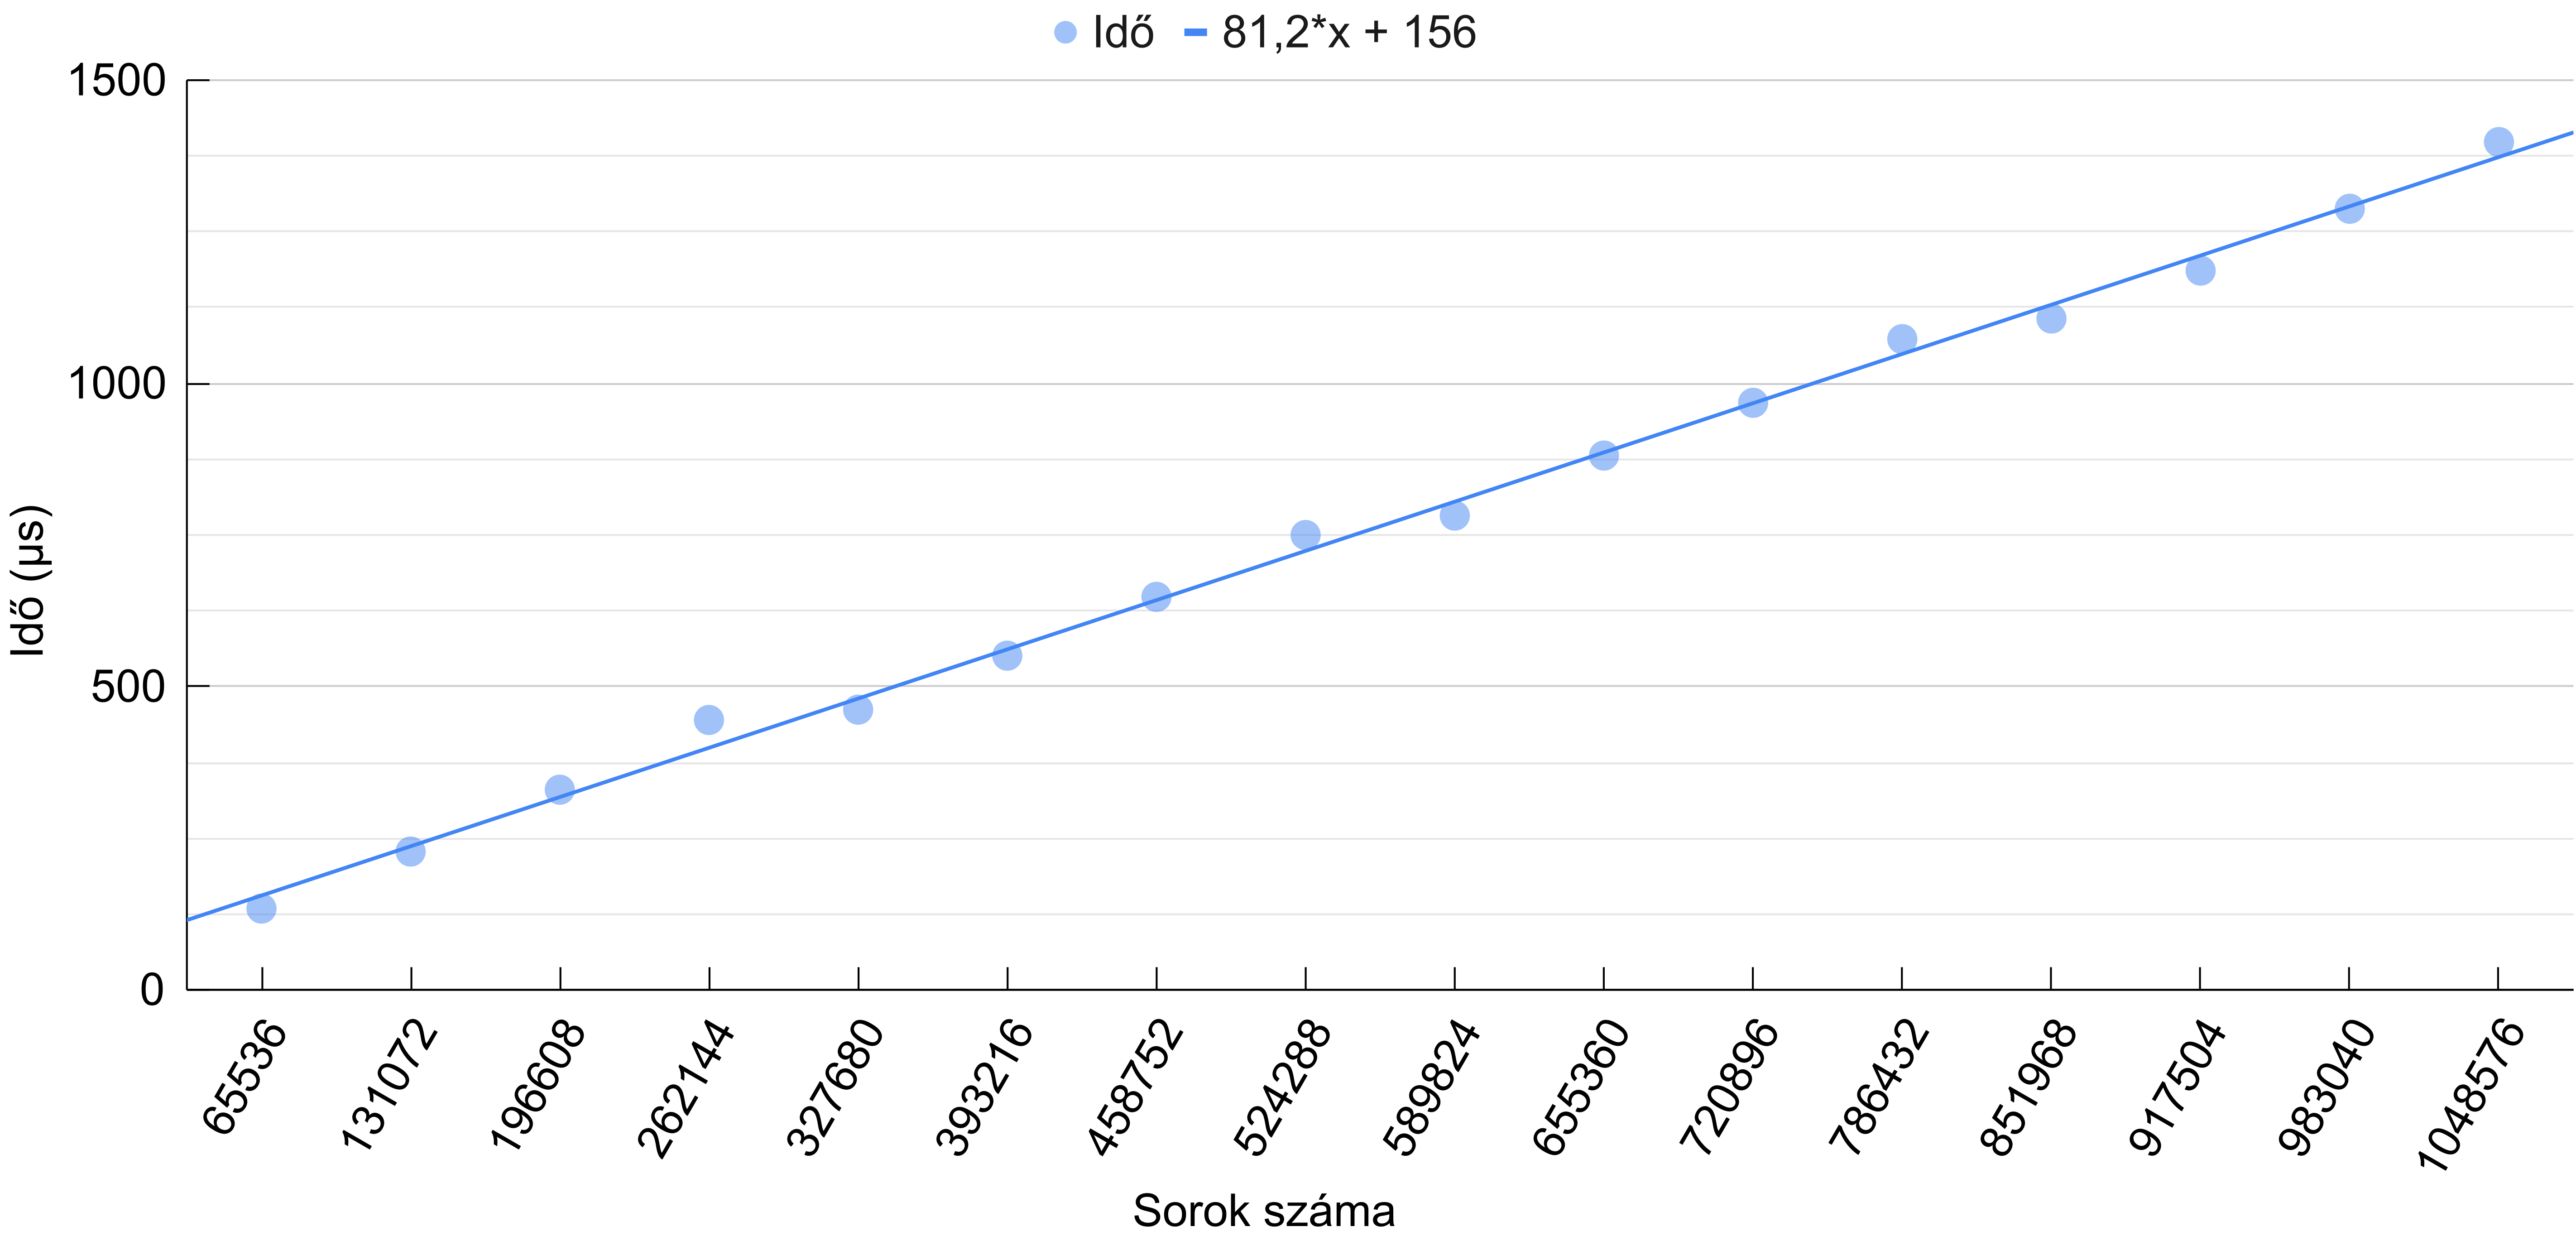
\includegraphics[width=14.8cm]{images/graph/pufferout.png}
	\caption{Adatok kimásolása 2.}
	\label{fig:pufferout}
\end{figure}

Fontos megjegyezni, hogy a mérések egy program futtatáson belül történtek. Ez azért olyan lényeges, mert operációs rendszer és egyéb memória kezelési tényezők miatt, az első kimásolás akár 25\%-al is lassabb lehet, mint az azt követőek, ugyan azon pufferből.

A másik módszer, miszerint nem olvassuk ki azonnal a teljes választ, hanem alkalmazzuk az előző fejezetben taglalt optimalizálási eljárást.
Ennek hatékonysága a sok kisebb olvasás miatt függ az eredmények számától. Ennek méréséhez módosítani kell a kernel kódot, ezért manuálisan végeztem a méréseket, vagyis a szűrési feltételeket úgy módosítottam, hogy a találatok száma megfelelően változzon.

\begin{figure}[h!]
\centering
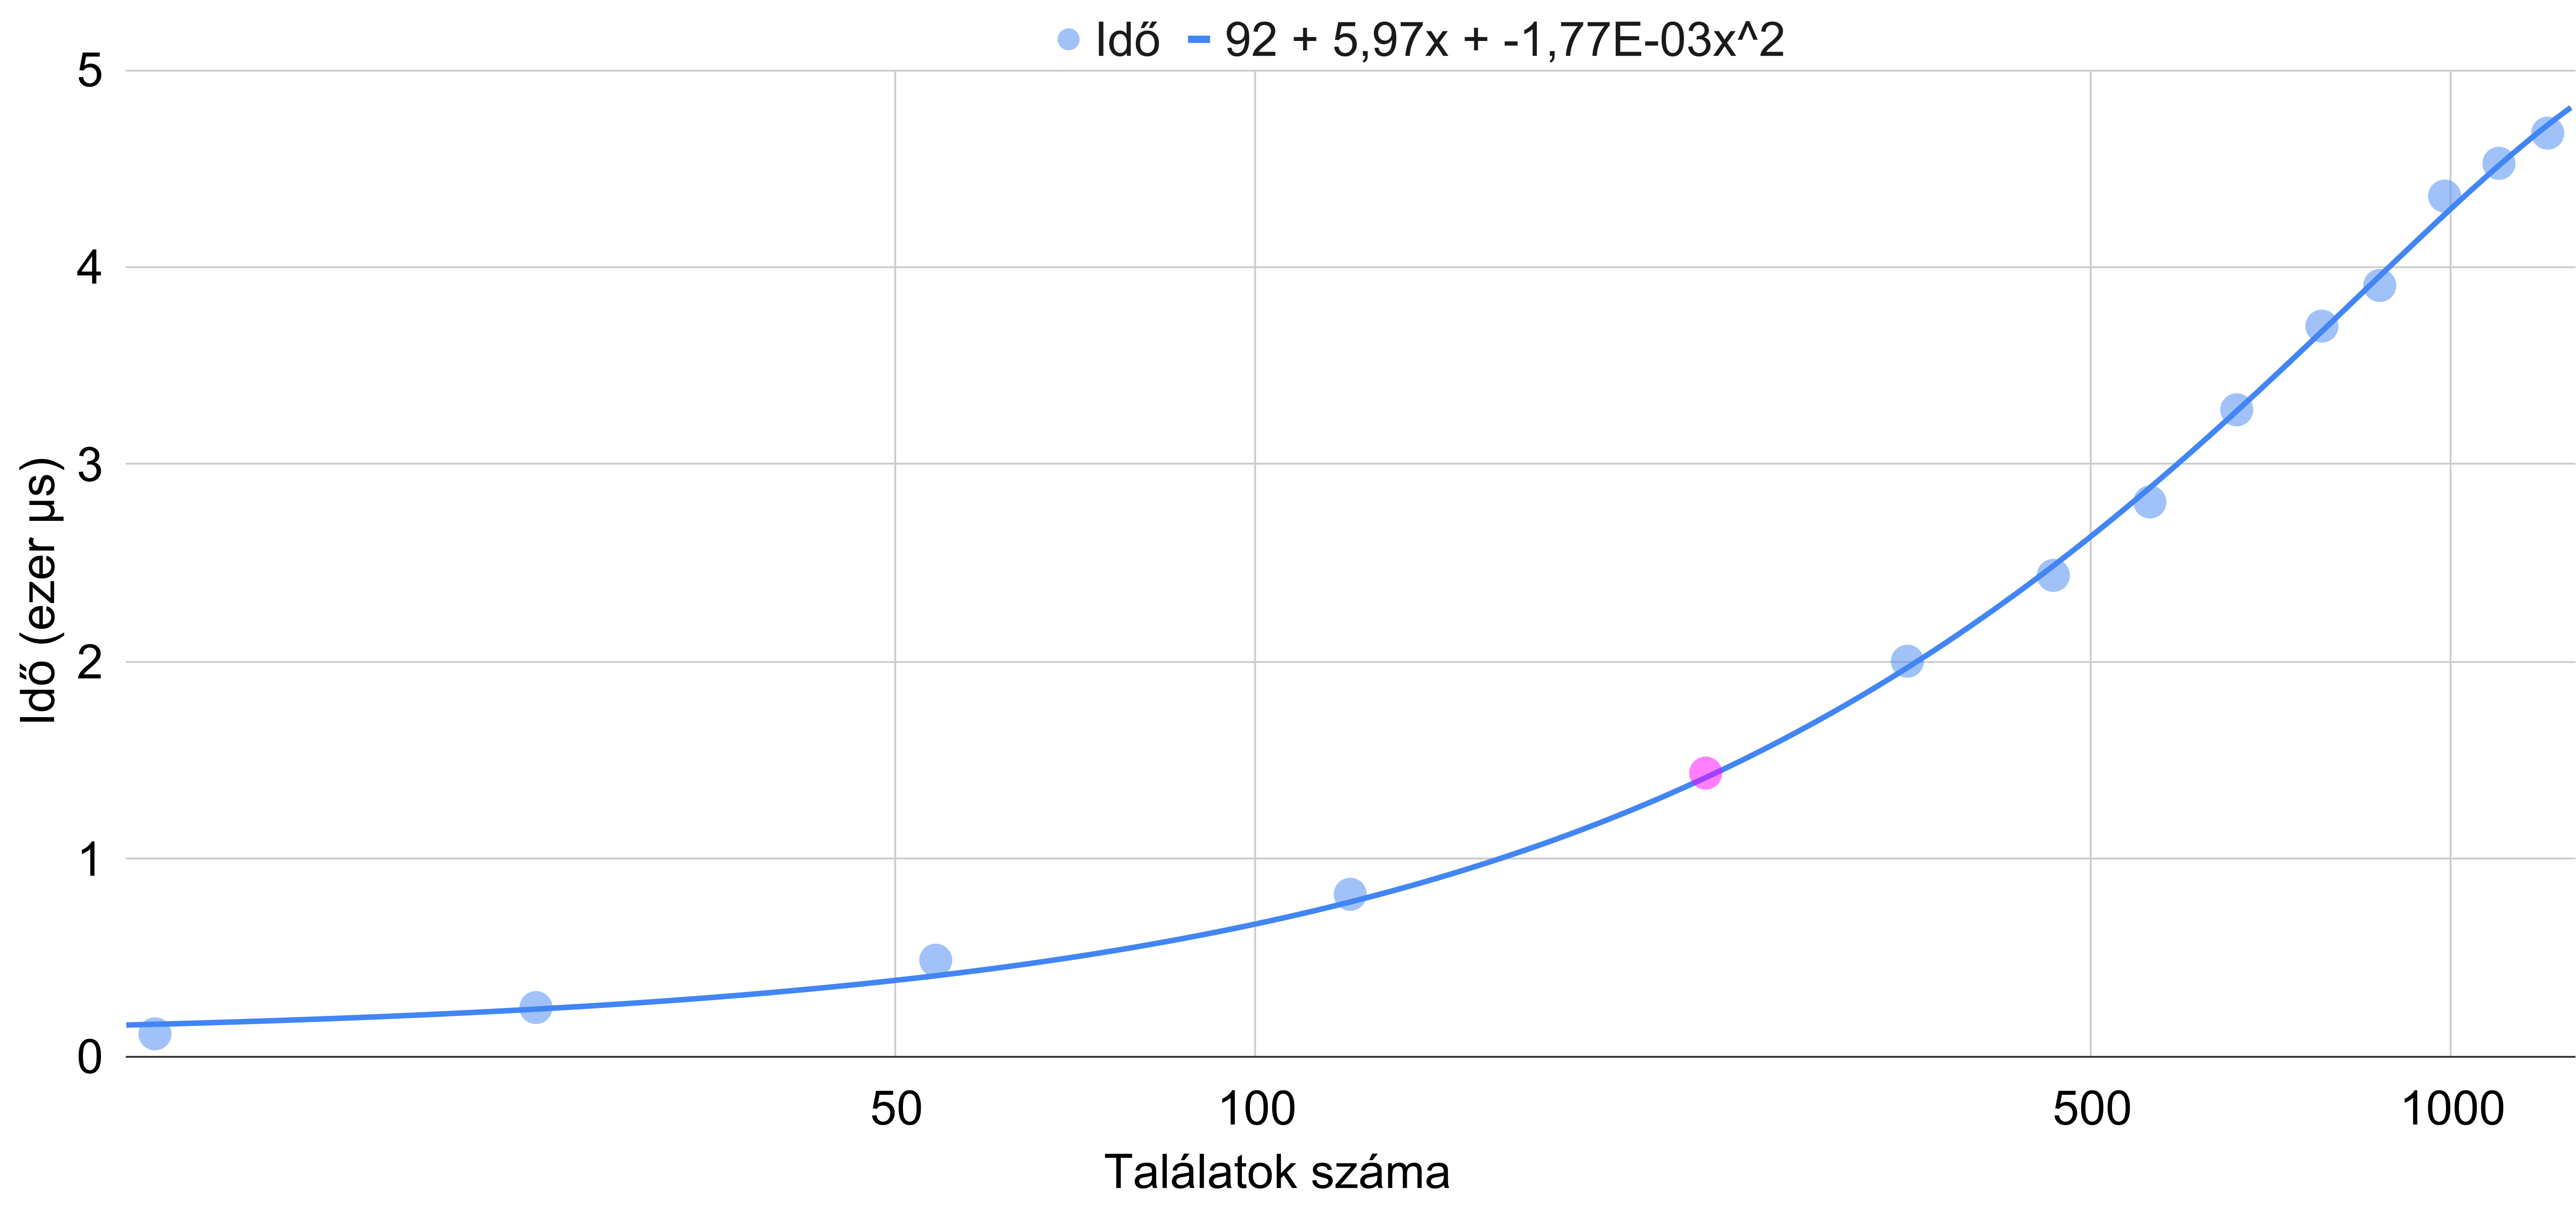
\includegraphics[width=14.8cm]{images/graph/outpuffer2_1.png}
\caption{Adatok kimásolása 2.}
\label{fig:outpuffer2_1}
\end{figure}

\begin{figure}[h!]
\centering
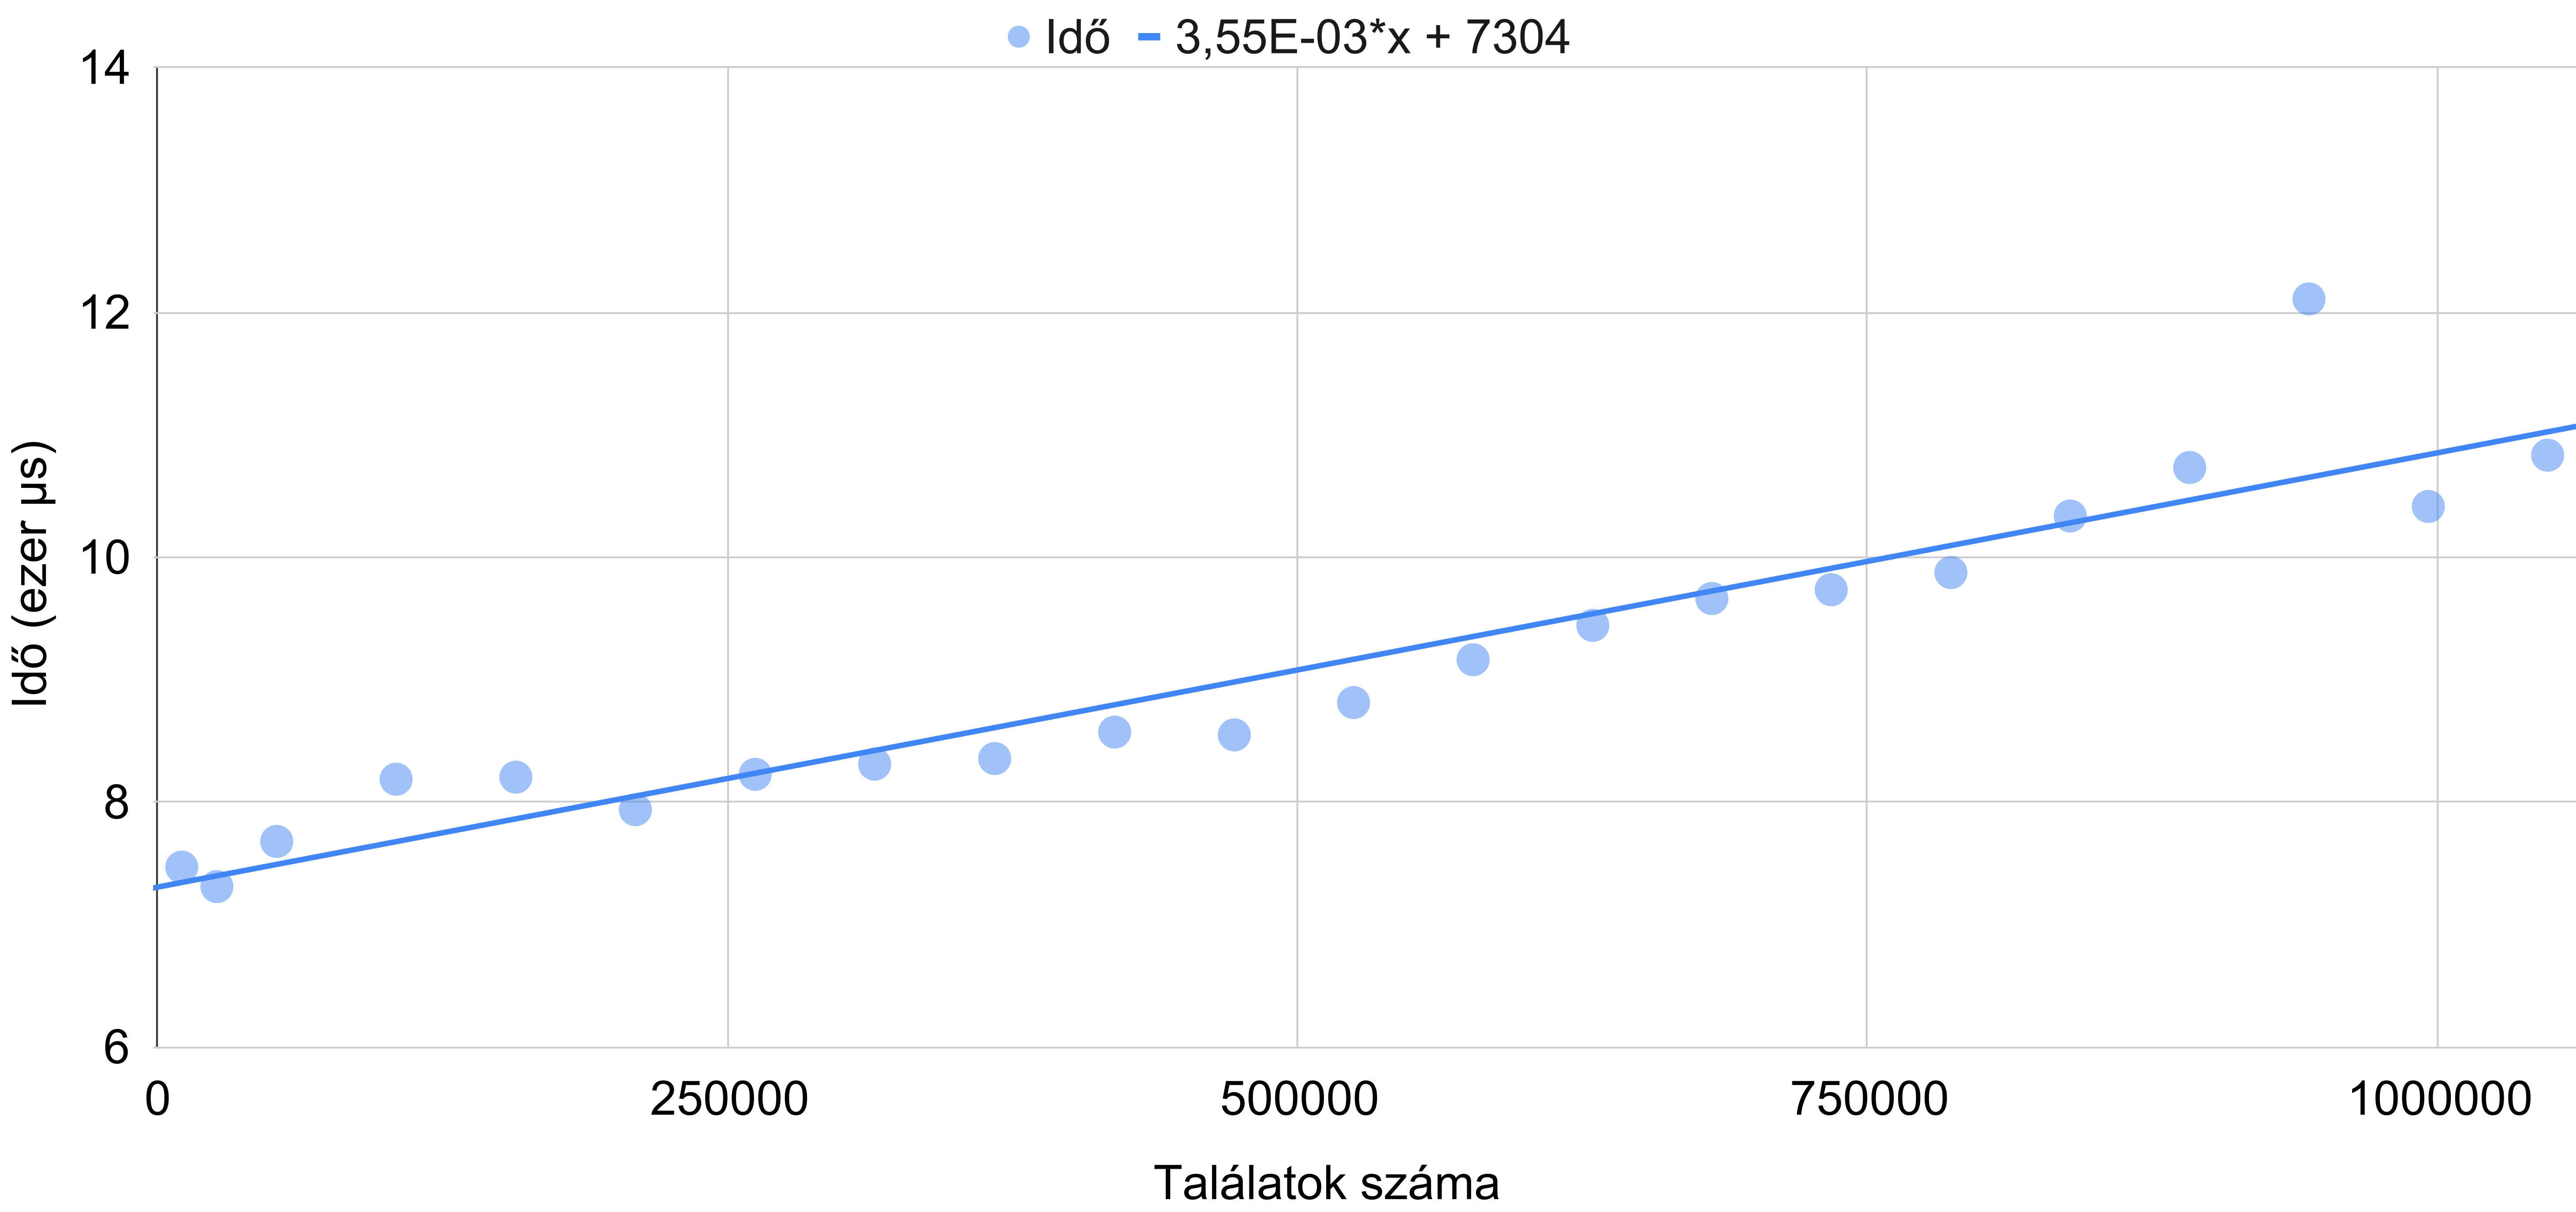
\includegraphics[width=14.8cm]{images/graph/outpuffer2_2.png}
\caption{Adatok kimásolása 2.}
\label{fig:outpuffer2_2}
\end{figure}

Végeredményként \aref{fig:outpuffer2_1}. és \aref{fig:outpuffer2_2}. ábrákon láthatjuk, hogy ez a fajta kiolvasás rendkívül hatékony, de csak abban az esetben, ha a találatok száma minimális.
238 találatnál a módszer elérte azt az időt, ami alatt el lehet végezni a teljes másolást egy darabban.

\SubSection{A globális méretből adódó sebességek}

A megfelelő globális méret meghatározása futási idő szempontjából nagyon fontos.
\noindent
A túl nagy globális méret hatásai a következők.
\begin{itemize}
\item A lokális méret korlátai miatt túl sok csoport jön létre, így azok feldolgozása soros lesz.
\item A kimeneti számláló mérete megnő, ennek kiolvasása több idő, és alacsony találati szám mellett a fölösleges ellenőrzések száma szignifikáns lehet.
\end{itemize}
\noindent
A túl alacsony globális méret hatásai pedig az alábbiak.
\begin{itemize}
\item A lokális méretet is szükséges lehet csökkenteni. Ha túl alacsony, akkor egyetlen munkaelem fogja végrehajtani, a párhuzamosság teljesen megszűnik.
\item A kimeneti számláló mérete alacsony, kevés visszatérő értéknél a kiolvasás gyors.
\end{itemize}
A méréseket ezen pontok alapján a következők szerint végeztem.
A globális méret változzon $[1, 2^{20}]$ tartományon, a lokális pedig $[1, 1024]$ tartományon négyzetes lépcsőkkel, az oszthatóságra figyelve.

A Gantt diagramhoz \texttt{gantt}, a további grafikonokhoz tartozó pedig \\
\texttt{global\_size\_speed} néven szerepel az elkészített programok között. Nézzük meg ezek működését!
\begin{python}  
timer.start();

clStatus = clEnqueueNDRangeKernel(command_queue, kernel, 1, NULL, 
	&global_size, &local_size, 0, NULL, NULL);

clStatus =
	clEnqueueReadBuffer(command_queue, Result_indexes_list_clmem, 
	CL_TRUE, 0, global_size* sizeof(int), 
	result_counter, 0, NULL, NULL);
	
clStatus = clEnqueueReadBuffer(command_queue, TableResult_clmem, 
	CL_TRUE, 0, t1_size * sizeof(TableResultType), 
	result, 0,NULL, NULL);

clStatus = clFinish(command_queue);
clStatus = clFlush(command_queue);

for(int i=0; i<global_size; i++)
{
    for (int j = 0; j < result_counter[i]; j++ );
}
myfile << timer.elapsedMicroseconds() << ",";  
\end{python}

Szembetűnő lehet az egymásba ágyazott két ciklus. Azért szerepel ez kódrészlet a mérésekbe, hogy az eredményeken való végiglépegetés idejének nagyságrendje valamilyen módon meghatározható legyen. Fontos megjegyezni, hogy a fordítás során nem kerül figyelmen kívül hagyásra ez a két ciklus.

\Aref{fig:gantt}. ábrán látható Gantt-diagram mutatja részletesen, hogy mely program szakasz mennyi időbe telik.
Minden esetben a lokális méret 32 és a visszatérő értékek száma körülbelül $50\%$, az eredményben pedig csak az index szerepel.

\begin{figure}[h!]
\centering
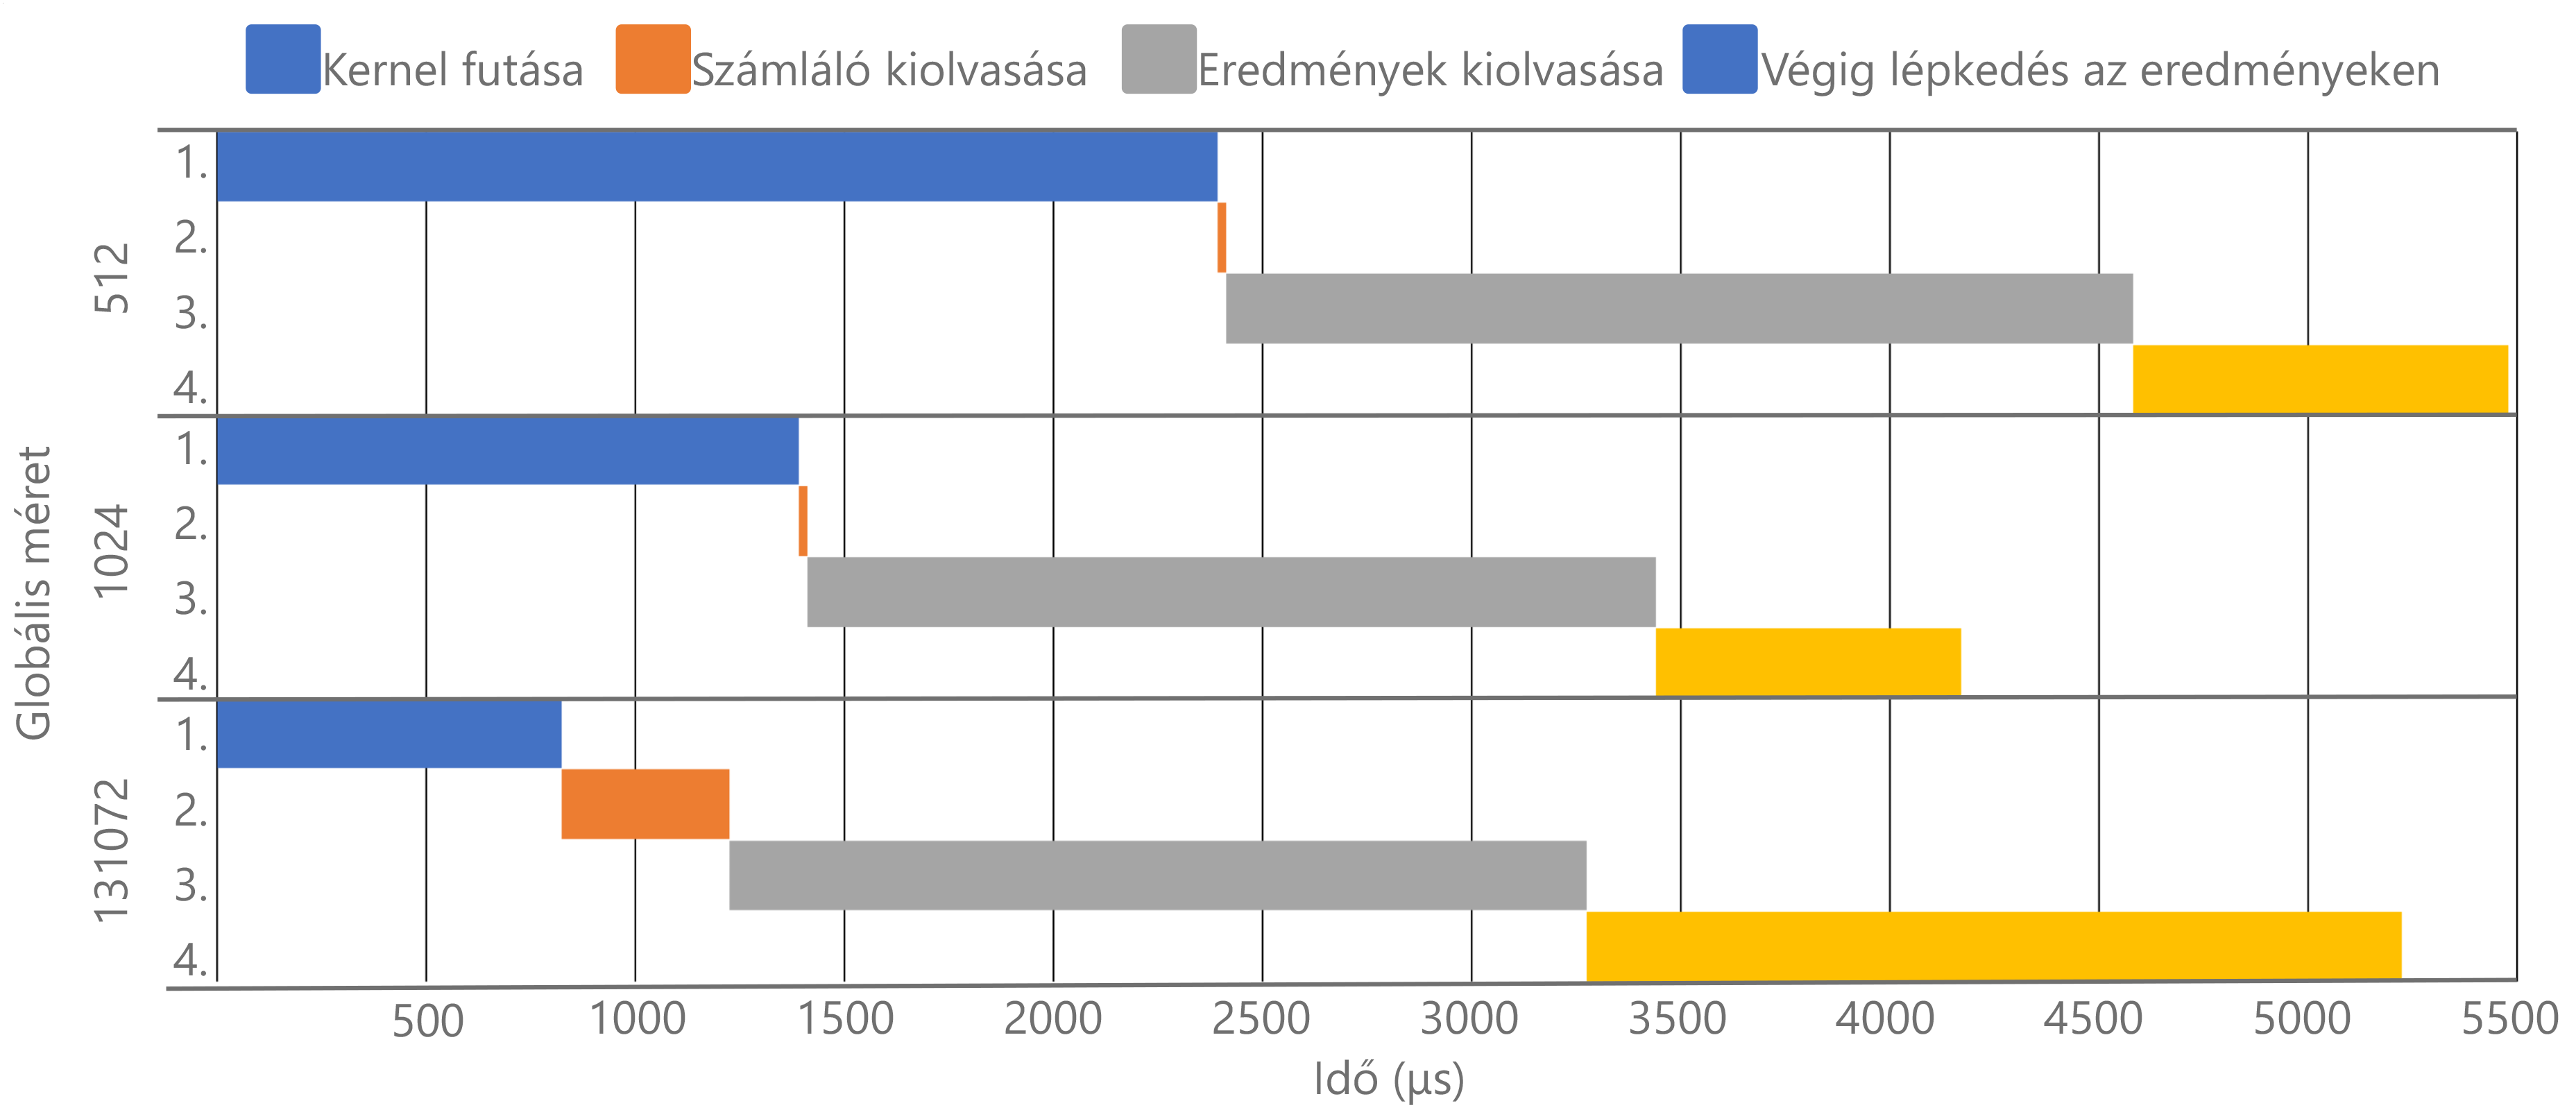
\includegraphics[width=\textwidth]{images/gantt.png}
\caption{Programszakaszok ideje.}
\label{fig:gantt}
\end{figure}

Látható, hogy a túl alacsony globális méret túl magas kernel futási időt eredményez. Túl nagy méret esetében pedig az eredmények kezelésének ideje válik számításigényessé.

(A diagram előállításához használt kód megtalálható a programok/\texttt{gantt} nevű mappában.)

\begin{figure}[h!]
\centering
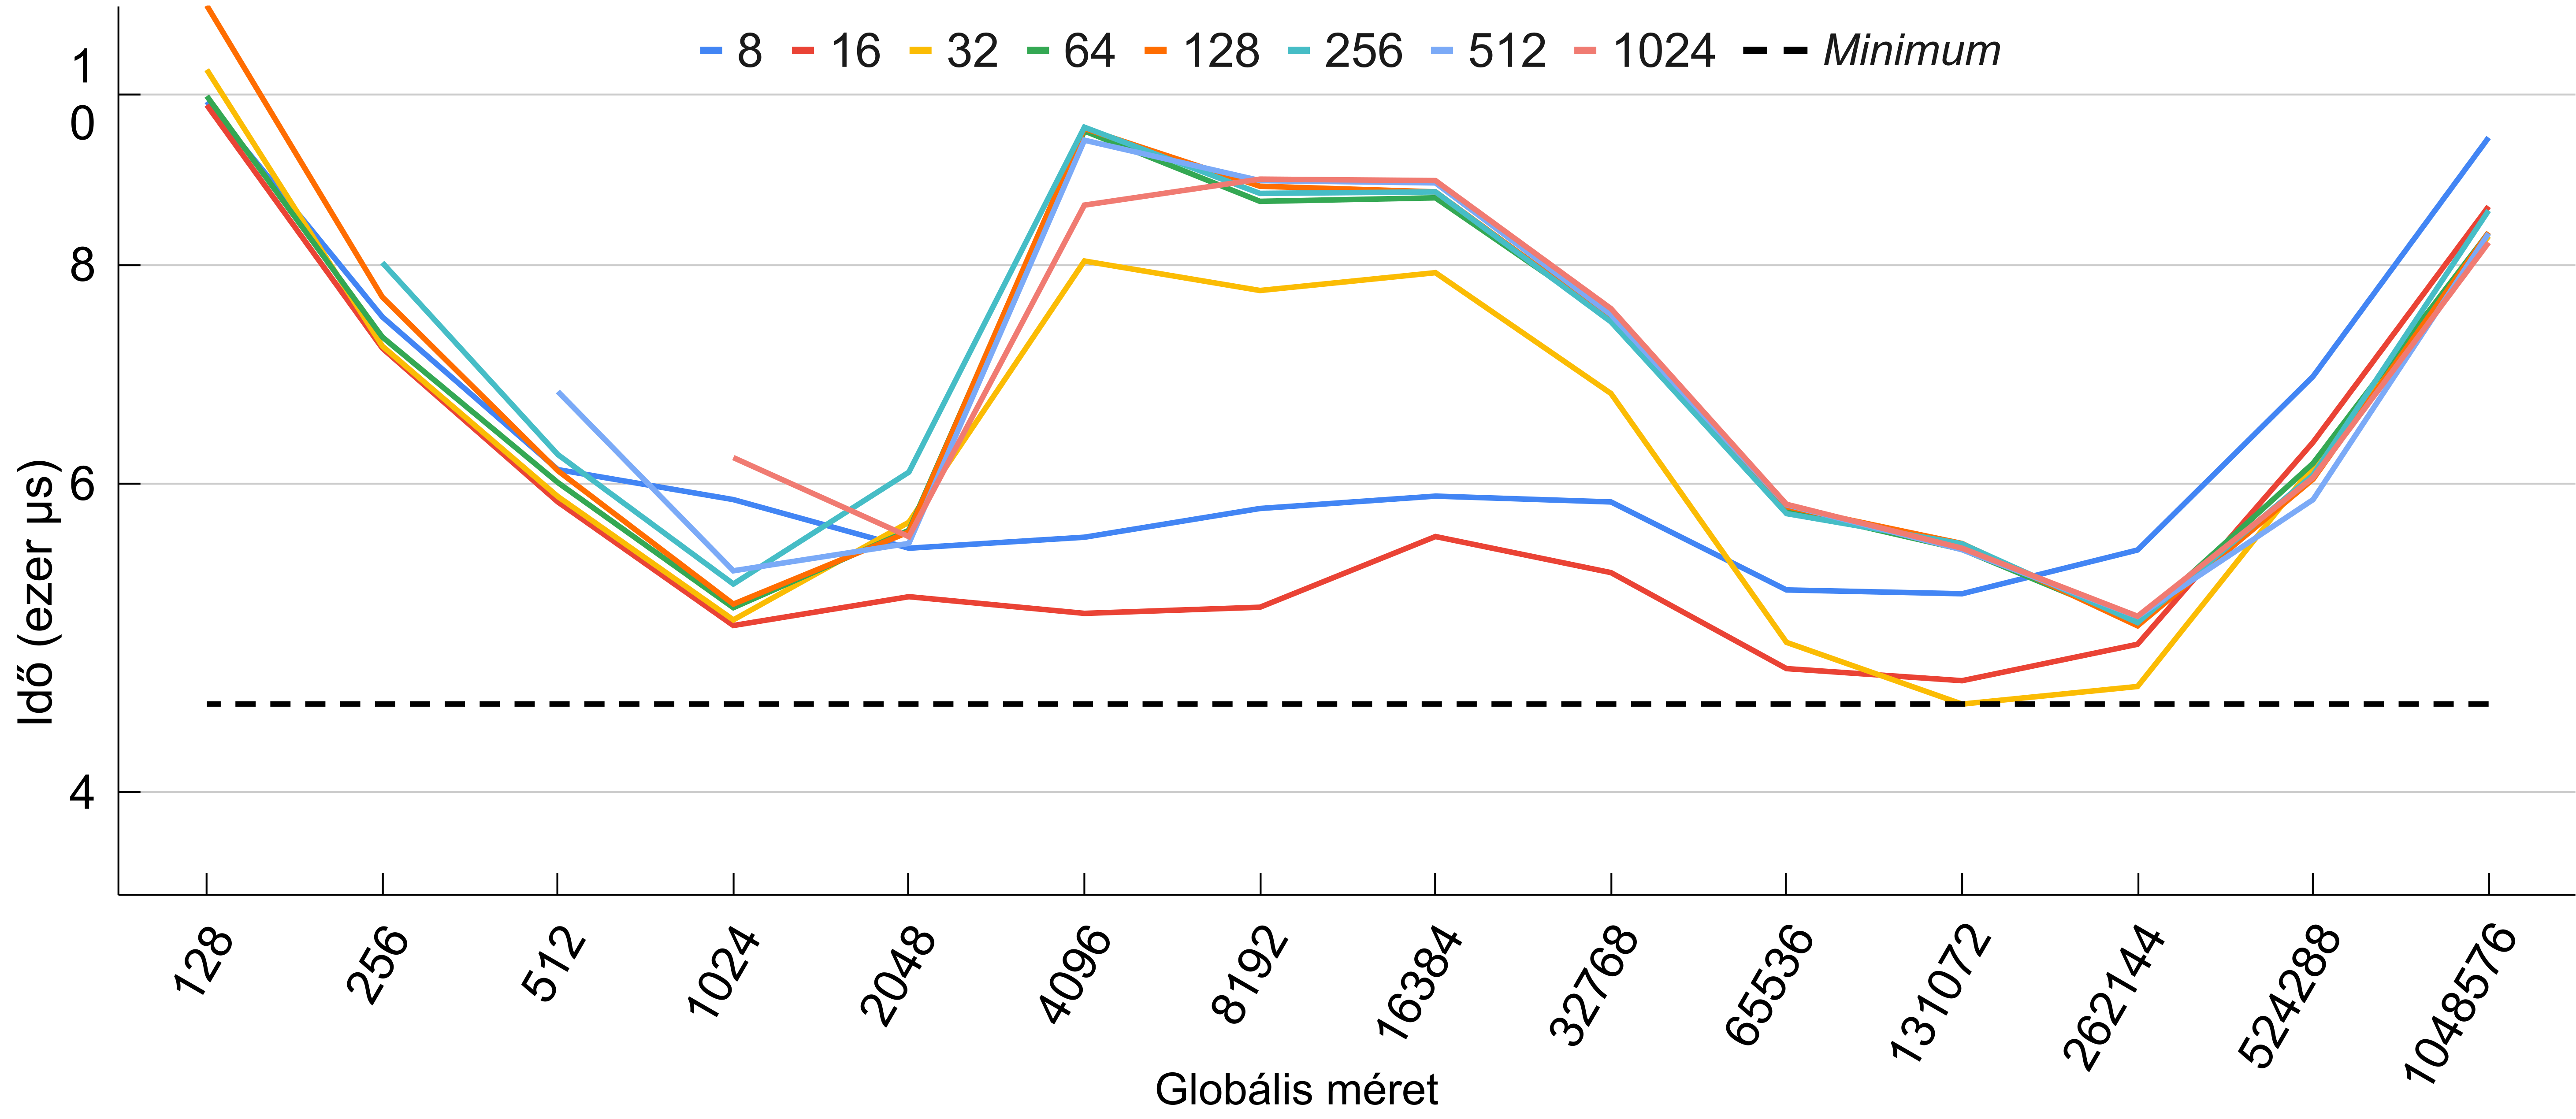
\includegraphics[width=\textwidth]{images/graph/global_size_1.png}
\caption{Maximális találat, az eredmény csak index.}
\label{fig:global_size_1}
\end{figure}

Az eredményt megvizsgálva látható, hogy van egy optimális globális méret tartomány $1024$ és $262144$ között (\ref{fig:global_size_1}. ábra).
Azt is észrevehetjük, hogy bizonyos lokális méretek ebben a tartományban drasztikusan rosszabb eredményt mutatnak.
A 16-os és 32-es méretek állnak legközelebb az ideális futási időhöz.

\begin{figure}[h!]
\centering
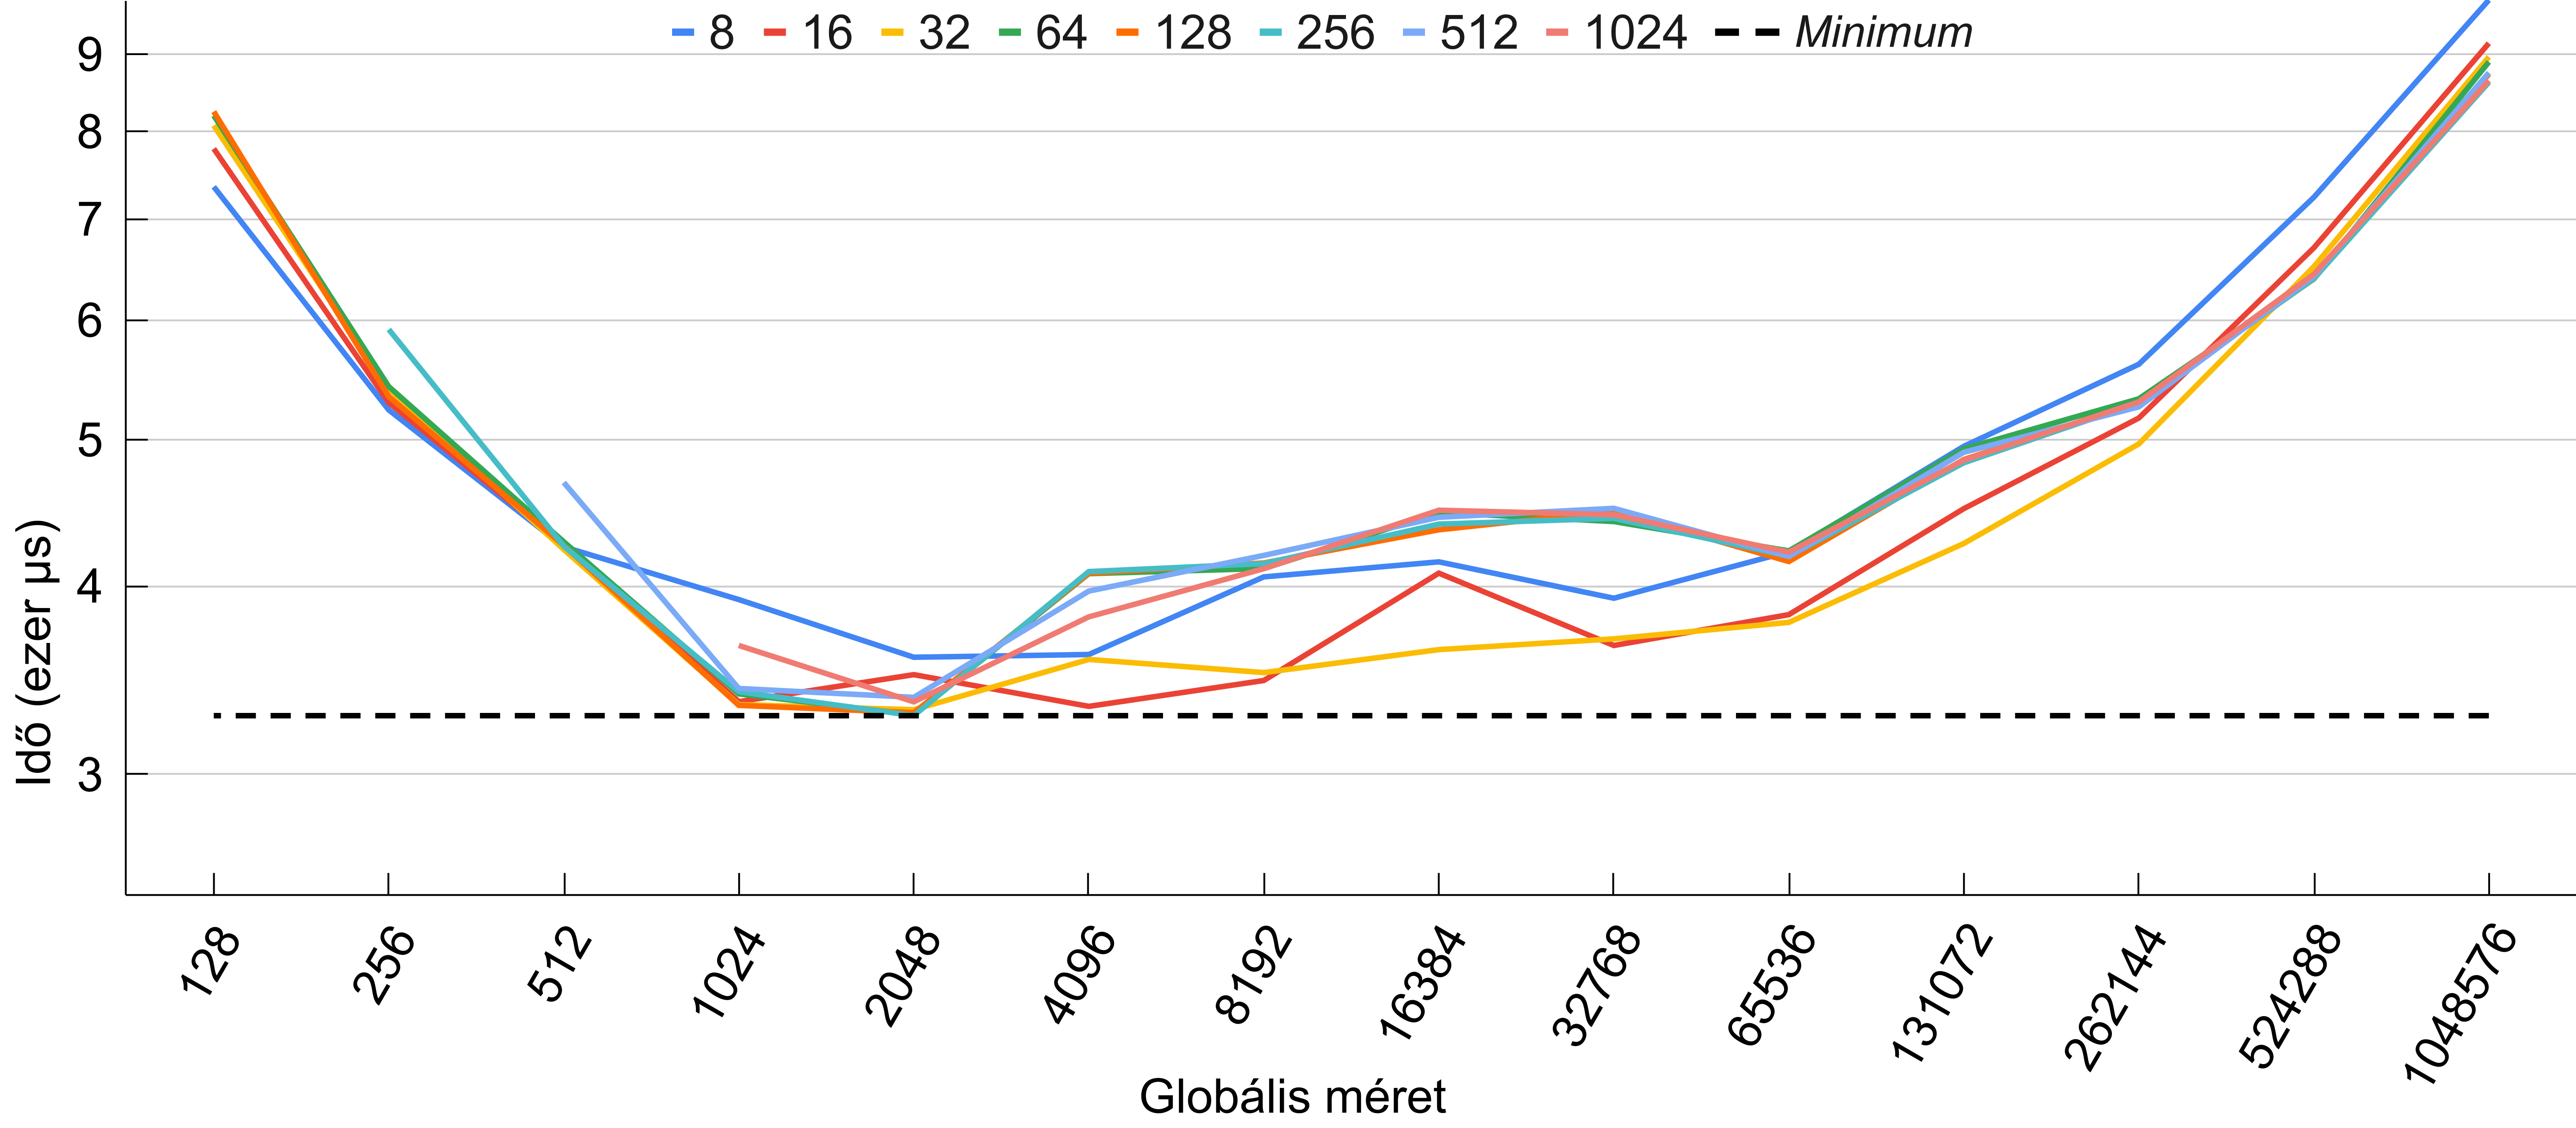
\includegraphics[width=\textwidth]{images/graph/global_size_2.png}
\caption{kb. 10\% találat, az eredmény csak index.}
\label{fig:global_size_2}
\end{figure}

\Aref{fig:global_size_2}. grafikonon egy olyan mérés látható, ahol a kernelben található feltételt úgy állítottam be, hogy megközelítőleg csak a tábla méretének 10\% -ával térjen vissza a lekérdezés.
Azt láthatjuk, hogy az előző középen lévő hullám lesimul, ez részben annak köszönhető, hogy a kernel futási ideje csökken azzal, hogy nem kell annyi indexet az eredmény tömbbe írnia.

Azoknál a lekérdezéseknél a kernelnek nem csak egy indexszel kell visszatérnie, hanem több kalkulált értékkel is, ott is hasonló grafikonokat kapunk. De a kernel növekvő munkája és a megnövekedett adatmennyiség kiolvasása miatt a középen lévő hullám nagyobb és nehezebben lapul le.

Ezek alapján azt mondhatjuk, hogy közel ideális választás volt az 1024 mint globális méret.

\Section{Gyakorlati példák és következtetések}

A hatékonyság megállapításához a \textit{A \texttt{MySQL} lekérdezés sebessége} részben használt módszert fogom alkalmazni.
A fejezetben előfordulnak rövidítések: CONN - a \texttt{MySQL Connector} programra a CL pedig az \texttt{OpenCL} -t használó programra utal. 
A k betű ezres szorzót, az i betű pedig indexelés használatot jelöl.
\newline Bontsuk az \texttt{OpenCL} programot négy részre:
\begin{itemize}
\item Előkészítés - Minden ami a kernel futása előtt történik,
\item Kernel(ek) futása,
\item Eredmények kiolvasása,
\item Eredmények kezelése.
\end{itemize}
A \texttt{Connector} programot pedig 3 részre:
\begin{itemize}
\item Előkészítés - Minden ami a kernel futása előtt történik,
\item Lekérdezés - A korában már említett két sor,
\item Eredmények kezelése.
\end{itemize}
Az eredmény kezelése résznél azt vizsgáljuk melyik esetben gyorsabb az eredményeket fájlba írni.

\SubSection{Egy táblás lekérdezés}

(Forrás: programok, \texttt{program\_test}/\texttt{where} mappa.)

\begin{python}
SELECT * FROM speedtest_1048576 WHERE c3 = 1 AND c4 > 5001;
	5307 row(s) returned
SELECT * FROM speedtest_1048576 WHERE c3 > 1 AND c4 > 5001;
	514025 row(s) returned
\end{python}
Először vizsgáljuk meg azt, mennyi ideig tart a lekérdezés, ha a Connenctor-t használjuk.

\begin{table}[h!]
\centering
\begin{tabular}{|p{6cm}|p{3cm}|p{3cm}|}
\hline
Sorok száma & 5307 & 514025 \\
\hline\hline

Előkészítés & 21237 $\mu s$ & 19125 $\mu s$ \\
\hline

Lekérdezés & 183674 $\mu s$ & 273130 $\mu s$ \\
\hline

Eredmény kiírás & 12591 $\mu s$ & 1110877 $\mu s$ \\
\hline
\end{tabular}
\end{table}

\noindent Ugyanez indexeléssel:

\begin{table}[h!]
\centering
\begin{tabular}{|p{6cm}|p{3cm}|p{3cm}|}
\hline
Sorok száma & 5307 & 514025 \\
\hline
\hline

Előkészítés & 21483 $\mu s$ & 16573 $\mu s$ \\
\hline

Lekérdezés & 23979 $\mu s$ & 268184 $\mu s$ \\
\hline

Eredmény kiírás & 17009 $\mu s$ & 1087573 $\mu s$ \\
\hline
\end{tabular}
\end{table}

\newpage

\noindent Illetve az \texttt{OpenCL} program használatakor:

\begin{table}[h!]
\centering
\begin{tabular}{|p{6cm}|p{3cm}|p{3cm}|}
\hline
Sorok száma & 5307 & 514025 \\
\hline
\hline
Előkészítés & 692705 $\mu s$ & 682227 $\mu s$ \\
\hline
Kernel futás & 1129 $\mu s$ & 1602 $\mu s$ \\
\hline
Eredmény kiolvasás & 2197 $\mu s$ & 2013 $\mu s$ \\
\hline
Eredmény kiírás & 11897 $\mu s$ & 916984 $\mu s$ \\
\hline
\end{tabular}
\end{table}

Láthatjuk, hogy összességében az \texttt{OpenCL} megvalósítás sokkal lassabb. De vegyük észre, hogy a program legtöbb részének csak egyszer kell lefutnia. 
Több lekérdezés végezhető úgy, hogy csak a  kernel és eredménykiolvasás idejét kell többszörözni. Ezen kívül szembetűnő az is, hogy a tömbben lévő adatokat gyorsabban lehet kezelni.

Úgy gondolom meg kell jegyezni azt is, hogy a tábla utólagos indexelése megközelítőleg 5,5 másodpercet vett igénybe.
\newline A hatékonyságot a következő módon becsülhetjük:
\begin{itemize}
\item Az előkészítést egyszer vesszük figyelembe.
\item Az előkészítési időhöz hozzá adjuk az ismétlődő részeket.
Lekérdezés, kernel(ek) futása, eredmény kiolvasás, eredmény kiírás.
\end{itemize}

\begin{figure}[h!]
\centering
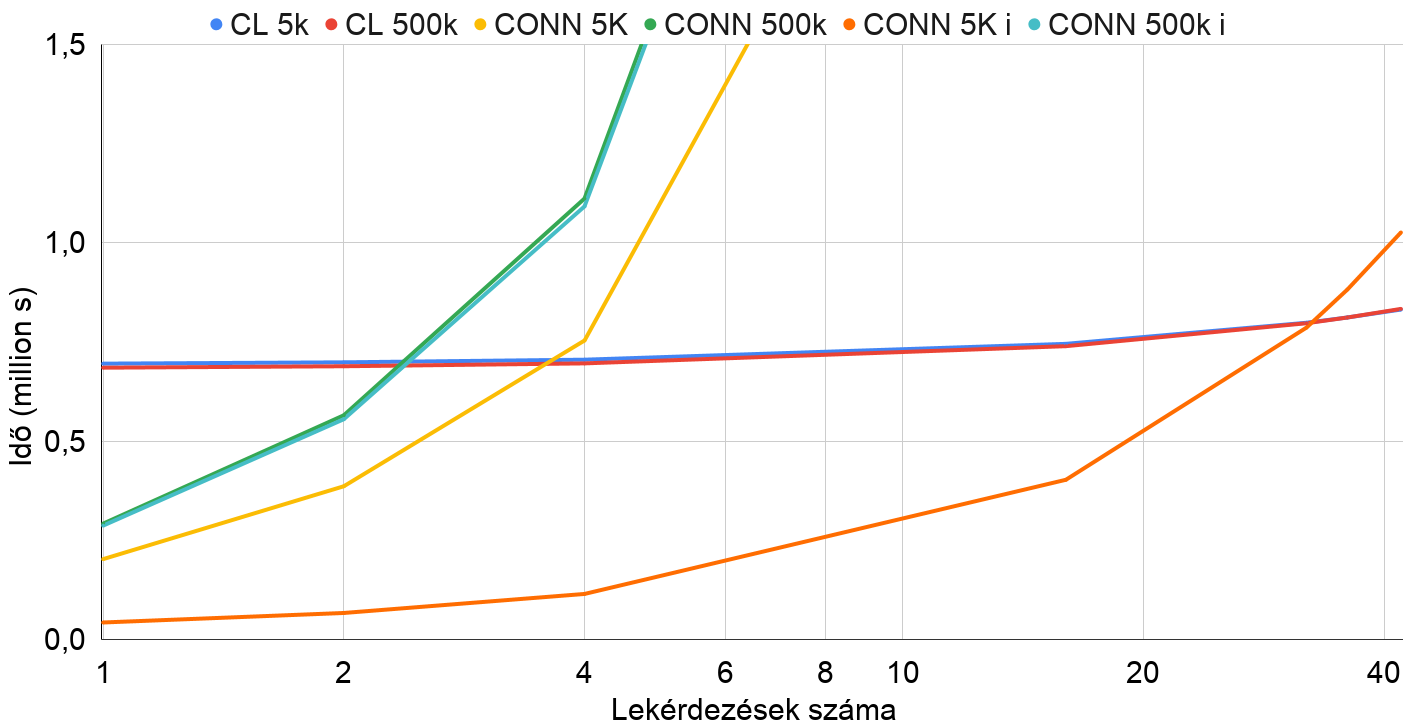
\includegraphics[width=\textwidth]{images/test/where3.png}
\caption{Becslés csak a lekérdezésre.}
\label{fig:where}
\end{figure}

\begin{figure}[h!]
\centering
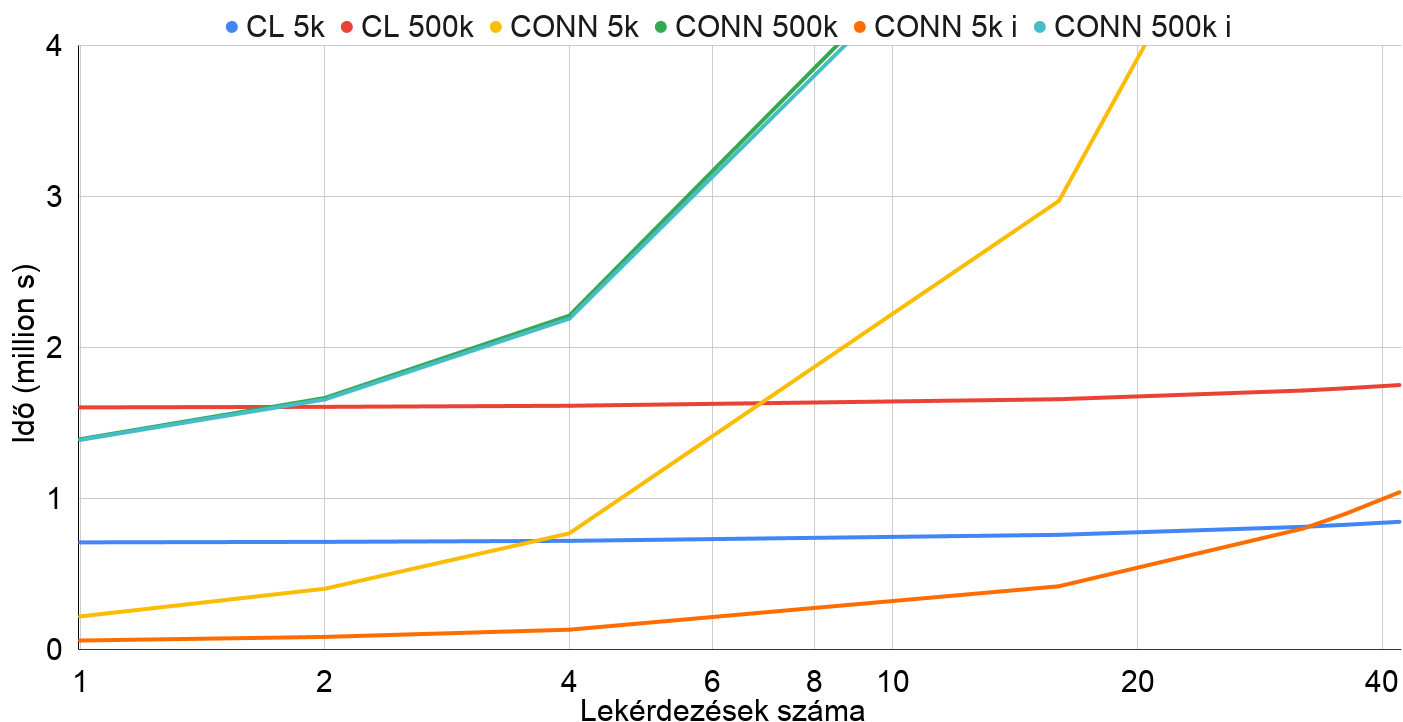
\includegraphics[width=\textwidth]{images/test/where_write3.png}
\caption{Becslés az eredmények kiírásával.}
\label{fig:where_write}
\end{figure}

A mérésekből a következő következtetéseket vonhatjuk le:
\begin{itemize}
	\item 0.5\%-os visszatérési arany esetében, ha nincs indexelés, akkor 7 lekérdezés után megtérülhetnek az \texttt{OpenCL} plusz költségei.
	\item Ha van indexelés abban az esetben ez a szám eléri a 37 -et.\newline
	50\%-os visszatérési aránynál már a 2. lekérdezésnél is nyereséges az \texttt{OpenCL} -es megvalósítás. 
\end{itemize}

\Aref{fig:where}. ábrán látható grafikonon a \texttt{CONN 500k} és \texttt{CONN 500k i} szinte egymást fedi, amiből látjuk, hogy ha a válaszban visszatérő sorok száma magas, akkor az indexelés hatékonysága alacsony.

\SubSection{Két táblás lekérdezés}
(Forrás: programok, \texttt{program\_test}/\texttt{join} mappa.)

Ehhez a részhez új adatbázist hoztam létre, az \texttt{EXPLAIN} bemutatásánál használthoz hasonlóan, de jelentősen nagyobb méretekkel, erre a tábla neve utal.
A generáláshoz szükséges kód megtalálható a \texttt{table gen} mappában.

\begin{python}
SELECT TM.c1p1, TS.c1p1, TM.c3 * TS.c3
FROM speed2.speed_262144 AS TM 
JOIN speed2.speed_131072 AS TS ON (TM.fk_s = TS.c1p1) 
WHERE TM.c3 > 9600 AND TS.c3 > 9200; 
	839 row(s) returned
...
WHERE TM.c3 > 9900 AND TS.c3 > 9900; 
	16 row(s) returned
\end{python}

A \texttt{Connector} mérési eredményei:

\begin{table}[h!]
\centering
\begin{tabular}{|p{6cm}|p{3cm}|p{3cm}|}
\hline
Sorok száma & 16 & 839 \\
\hline\hline

Előkészítés & $21425 \mu s$ & $21893 \mu s$ \\
\hline

Lekérdezés & 39363 $\mu s$ & 85889 $\mu s$ \\
\hline

Eredmény kiírás & 90 $\mu s$ & 2120 $\mu s$ \\
\hline

\end{tabular}
\end{table}

\newpage

Indexeléssel:

\begin{table}[h!]
\centering
\begin{tabular}{|p{6cm}|p{3cm}|p{3cm}|}
\hline
Sorok száma & 16 & 839 \\
\hline
\hline

Előkészítés & 20984 $\mu s$ & 26650 $\mu s$ \\
\hline

Lekérdezés & 10119 $\mu s$ & 31663 $\mu s$ \\
\hline

Eredmény kiírás & 97 $\mu s$ & 2802 $\mu s$ \\
\hline

\end{tabular}
\end{table}

\texttt{OpenCL} megvalósítás

\begin{table}[h!]
\centering
\begin{tabular}{|p{6cm}|p{3cm}|p{3cm}|}
\hline
Sorok száma & 16 & 839 \\
\hline
\hline
Előkészítés & 314073 $\mu s$ & 315964 $\mu s$ \\
\hline
Kernel 1. 2. futása & 559 $\mu s$ & 593 $\mu s$ \\
\hline
Kernel 3. futása & 7662 $\mu s$ & 103988 $\mu s$ \\
\hline
Eredmény kiolvasás & 1974 $\mu s$ & 1745 $\mu s$ \\
\hline
Eredmény kiírás & 161 $\mu s$ & 1932 $\mu s$ \\
\hline
\end{tabular}
\end{table}	

Az \texttt{OpenCL} -es futási időket igyekeztem optimalizálni azzal, hogy a szerverről csak a szükséges oszlopokat kértem le, így elkerülve a fölösleges adatok mozgatását.

\begin{figure}[h!]
\centering
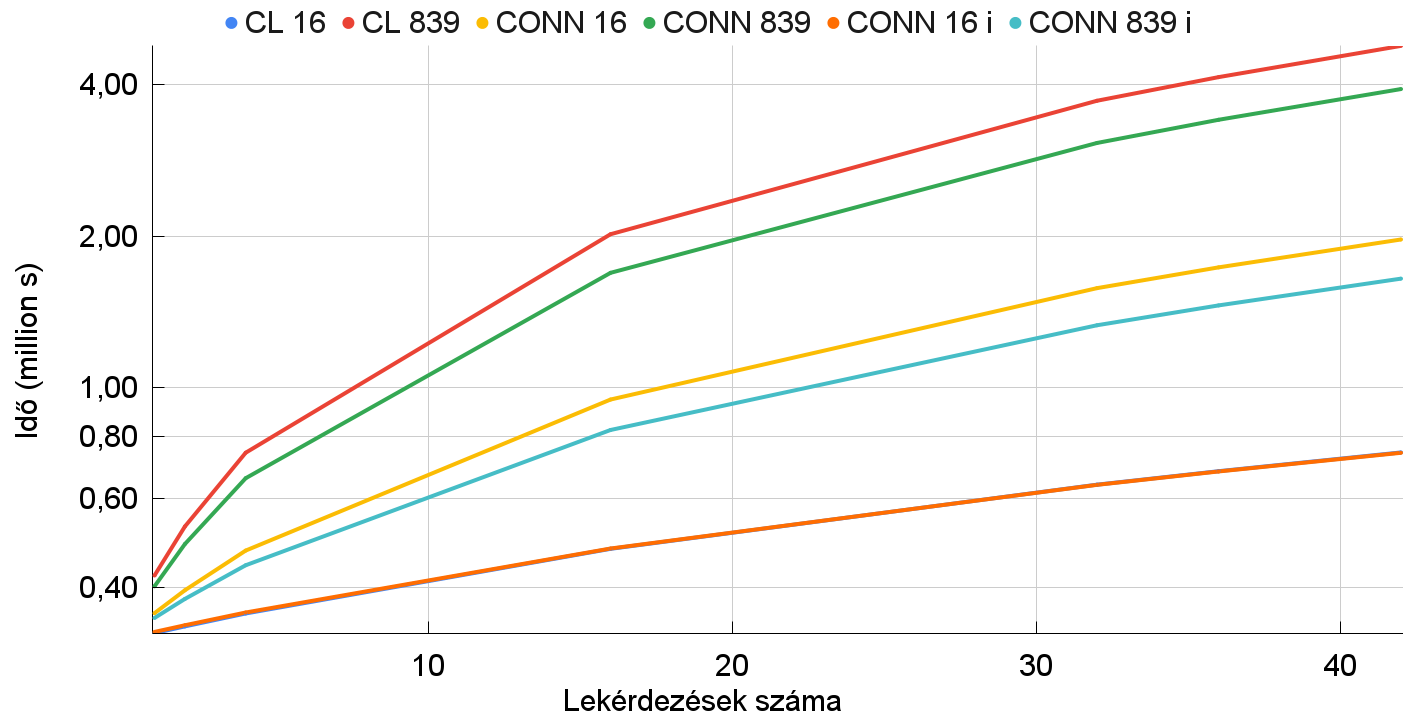
\includegraphics[width=\textwidth]{images/test/join2.png}
\caption{Becslés csak a lekérdezésre.}
\label{fig:join}
\end{figure}

\Aref{fig:join}. ábrán a méréseket látva, arra a következtetésre juthatunk, hogy az \texttt{OpenCL} program nem bizonyul hatékonynak, még ilyen alacsony találati számnál sem. A kiolvasási időt tovább lehetne optimalizálni az előzőekben említett másik módszerrel, ezzel akár tizedére is csökkenhet a kiolvasási idő, illetve minimálisan javulhat a kiírási idő is. Ez a kis számú lekérdezés annyira speciális esete lenne a lekérdezéseknek, hogy nem vizsgálom tovább.

A táblakapcsolás nélküli lekérdezéshez viszonyított drámai teljesítmény romlás oka az, hogy a \texttt{MySQL} motorja a táblák kapcsolásánál felhasználja a másodlagos kulcsokat, mint index, így nem kell végignéznie minden sort a párokat keresve.

Valamilyen indexelési módszer használatával az \texttt{OpenCL} megvalósítás is optimalizálható lenne, ám ez bonyolult és költséges lehet.

A \Aref{fig:join} ábrán jól látható, hogy már 839 visszatérő sornál is a CL megvalósítás a leglassabb. A 16 soros lekérdezés pedig alig előzi meg az indexelt lekérdezést.
Az eredményekből azt is látjuk, hogy nagyobb mértékben nőtt a futási ideje a CL programnak, azaz még több visszatérő sor eseten a módszer még kevésbé hatékony.

\Chapter{Összefoglalás}

A dolgozatban sok érdekes információ kiderült a mysql lekérdezések és az opencl -es megvalósítások hatékonyságával kapcsolatban.

A MySQL Workbench által előállított grafikus végrehajtási terv hatékonyan nyújt segítséget a lekérdezéseink optimalizálásához. Használatával egyszerű módon találhatjuk adatbázisunk hiányosságait, legyen az a felépítéséből vagy akár csak egy indexelés hiányából adódó hátrány. Ez az eszköz bárki számára könnyedén elérhető és sok esetben nem igényel különleges szaktudást sem. Ideális esetben akár egy indexelés hozzáadásával is töredékére csökkenthetjük lekérdezéseink idejét.

Áttérve a lekérdezések OpenCL -es megvalósítására, azt a következtetést vontam le, hogy vannak olyan esetek, amikor sebesség szempontjából jelentős előnyre lehet szertetenni ha kihasználjuk a grafikus kártyák teljesítményét. De ahhoz, hogy ez a gyakorlatban is megvalósítható legyen nagyon sok előzetes vizsgálatra van szükség. A hatékonyság függ:
\begin{itemize}
\item Az adatbázis szerver sebességétől.
\item A kliensgép erőforrásaitól.
\item A lekérdezés bonyolultságától.
\item A séma felépítésétől.
\end{itemize}

Erre megoldást nyújthat egy a proxy modell-el felépített kliens alkalmazás. Ennél dönthet a felhasználó arról, hogy bekapcsolja az \texttt{OpenCL} -es feldolgozót, vagy rábízhatja a programra ezt a döntést. A kiértékelőt egyedileg be kell paraméterezni adott sémához. A döntéshez többek között szükség van a a táblák felépítésre és arra, mely oszlopok indexeltek. De rengeteg minden egyéb is megadható, mint egy oszlop lehetséges értéktartománya vagy akár az adatok várható eloszlása, mellyel becsülhető egy szűrő szélessége. 

Egy ilyen kliensalkalmazás megírása rendkívül bonyolult és időigényes ezért nagyon kevés olyan eset lehet, ahol ez a befektetett idő és energia valóban megtérül. 


\clearpage

\addcontentsline{toc}{chapter}{Irodalomjegyzék}
\bibliographystyle{plain}
\bibliography{dolgozat.bib}

\newpage

\pagestyle{empty}

\noindent \textbf{\Large CD Használati útmutató}

\vskip 1cm

\noindent A CD-lemez tartalma

\begin{itemize}
    \item \textbf{dolgozat.pdf}
        \begin{itemize}
            \item A szakdolgozat PDF formátumban.
        \end{itemize}
	\item \texttt{programok/}
		\begin{itemize}
			\item Ebben a mappában találhatóak a felhasznált kódok illetve a méréseket tartalmazó táblázatok.
			\item README.txt fájl leírja, hogy az egyes könyvtárakban lévő programok mire szolgálnak és mi található bennük.
		\end{itemize}
	\item \texttt{szakdolgozat/}
		\begin{itemize}
			\item Itt találhatóak meg a dolgozat forrás fájljai.
		\end{itemize}
	\item \texttt{utmutato.pdf}
    \begin{itemize}
        \item Útmutató a CD használatához.
    \end{itemize}
\end{itemize}

%Ennek a címe lehet például \textit{A mellékelt CD tartalma} vagy \textit{Adathordozó használati útmutató} is.

%Ez jellemzően csak egy fél-egy oldalas leírás.
%Arra szolgál, hogy ha valaki kézhez kapja a szakdolgozathoz tartozó CD-t, akkor tudja, hogy mi hol van rajta.
%Jellemzően elég csak felsorolni, hogy milyen jegyzékek vannak, és azokban mi található.
%Az elkészített programok telepítéséhez, futtatásához tartozó instrukciók kerülhetnek ide.
%
%A CD lemezre mindenképpen rá kell tenni
%\begin{itemize}
%\item a dolgozatot egy \texttt{dolgozat.pdf} fájl formájában,
%\item a LaTeX forráskódját a dolgozatnak,
%\item az elkészített programot, fontosabb futási eredményeket (például ha kép a kimenet),
%\item egy útmutatót a CD használatához (ami lehet ez a fejezet külön PDF-be vagy MarkDown fájlként kimentve).
%\end{itemize}


\end{document}
